\supplementarysetup
Supplementary Methods provide the algorithm, formal properties, implementation details, and evaluation protocols; figures, tables, and machine-readable audits report the complete analyses. Archived legacy-compatible results remain distinct from corrected-objective results. The tuned-evaluator sensitivity and computational provenance in \crefrange{fig:supp21}{fig:supp22} are descriptive and do not support a core claim.


\section{Supplementary Methods}

\subsection{Complete WrapEvoFS algorithm}

\noindent\textbf{Complete development-only WrapEvoFS search and regret-constrained representative locking.}\par\smallskip
{\small
\renewcommand{\arraystretch}{1.12}
\setlength{\tabcolsep}{3pt}
\renewcommand{\theHtable}{suppalgorithm.\thealgorithm}
\begin{longtable}{@{}>{\centering\arraybackslash}p{0.055\linewidth}>{\raggedright\arraybackslash}p{0.895\linewidth}@{}}
\toprule
 & \textbf{Input.} Development data $(X_D,y_D)$; Direct candidates $\mathcal C_m$; RFECV configuration; GA mode and base seed $\xi_0$; population size $N$; generations $G$; runs $R$; elite count $e$; crossover probability $p_c$; per-bit mutation probability $p_\mu$; initial off-ratio $\rho_0$; locking metric and seed; tolerance mode and $\delta$. \\
 & \textbf{Output.} RFECV target $k_m^*$; locked set $F_m^{\mathrm{lock}}$; complete audit $A_m$. \\
\addlinespace[2pt]
1 & Fit preprocessing and Direct selection on development data only. \\
2 & Evaluate the eligible RFECV path and select $k_m^*$; resolve score ties toward the smaller count. \\
3 & Construct fixed stratified development folds for GA evaluation. Use zero-based indices $(r,g,i,\ell)$ in the seed definitions below. \\
4 & \textbf{For each} independent run $r=0,\ldots,R-1$, initialize the genetic-operator generator with seed $\xi_0+r$. \\
5 & \hspace*{1.35em}\textbf{For each} of $N$ initial chromosomes, set exactly $\lfloor\rho_0p_m\rfloor$ entries to zero and the remainder to one, uniformly shuffle their positions, and activate one uniformly sampled feature if an empty mask would otherwise result. \\
6 & \hspace*{1.35em}\textbf{For each} generation $g=0,\ldots,G-1$: \\
7 & \hspace*{2.70em}\textbf{For each} chromosome at population-list index $i$, compute its $K_G$ fold scores with random-forest seed $\xi_{rgi\ell}=\xi_0+10000r+100g+1009i+\ell$ in fold $\ell$. \\
8 & \hspace*{2.70em}Compute the mean base score, target deviation, penalty, raw objective, and zero-truncated legacy fitness. \\
9 & \hspace*{2.70em}\textbf{If corrected-objective mode:} rank and update run best by raw objective, base score, smaller deviation, smaller count, and stable mask hash. \\
10 & \hspace*{2.70em}\textbf{If legacy-compatible mode:} reproduce zero-truncated ranking and update behavior. \\
11 & \hspace*{2.70em}Copy the first $e$ ranked chromosomes unchanged to the next generation. \\
12 & \hspace*{2.70em}For the remaining $N-e$ positions, compute shifted proportional weights in corrected-objective mode (zero-truncated nonnegative weights in legacy-compatible mode) and normalize them to parent probabilities. \\
13 & \hspace*{2.70em}\textbf{If} weights are nonfinite, effectively equal, or have invalid or effectively zero total, set all parent probabilities to $1/N$ and record the fallback. \\
14 & \hspace*{2.70em}Sample $N-e$ parent indices independently with replacement and pair the sampled parents in list order. \\
15 & \hspace*{2.70em}For each pair, perform one-point crossover with probability $p_c$; when $p_m>2$, sample the cut uniformly from $\{1,\ldots,p_m-2\}$, otherwise copy both parents. \\
16 & \hspace*{2.70em}Independently flip every child bit with probability $p_\mu$; if a child is empty, activate one uniformly sampled feature. \\
17 & \hspace*{2.70em}Form the next size-$N$ population from the $e$ elites followed by mutated children; export generation diagnostics and warnings for zero truncation, deviation, sampling fallback, and mask collapse. \\
18 & \hspace*{1.35em}\textbf{End for} generation; retain one run-best candidate. \\
19 & \textbf{End for} run. \\
\addlinespace[2pt]
20 & Construct one fixed stratified locking-fold partition and re-score every retained run-best candidate with the same locking metric, fold partition, and random-forest hyperparameters, using its recorded run-specific estimator seed, to obtain $L_r$ and fold scores. \\
21 & Encode every candidate in the common ordered feature universe, compute its stable mask identifier, and compute $R_r=L_{\mathrm{best}}-L_r$ (plus configured sensitivity quantities). \\
22 & For the primary absolute rule, form $E_\delta=\{r:R_r\leq\delta\}$. Prespecified relative and best-run-SE-scaled modes form their corresponding sensitivity pools under their own declared thresholds. Never add a candidate outside the active threshold. \\
23 & \textbf{If} $|E_\delta|=1$, select its sole candidate. \\
24 & \textbf{Otherwise,} compute pairwise Jaccard similarity and each candidate's mean Jaccard within $E_\delta$. \\
25 & Select the medoid by larger mean Jaccard, larger $L_r$, smaller feature count, and lexicographically smaller stable mask hash; use source-run ID only as post-selection provenance among exact duplicate masks. \\
26 & Assert that the selected candidate is in $E_\delta$ and satisfies the exact declared threshold; export canonical masks and hashes, duplicate multiplicity and provenance, scores, fold scores, regrets, eligibility, Jaccard values, tie path, seeds, version, and configuration hash. \\
27 & \textbf{Return} $(F_m^{\mathrm{lock}},k_m^*,A_m)$. Held-out data are not inputs and are used only for one-time evaluation after the feature set, settings, and final model-development procedure are locked. \\
\bottomrule
\end{longtable}
\addtocounter{table}{-1}
}


Held-out data are excluded from search, rescoring, eligibility, locking, and audit export. Executable v0.2.0 specifications are consolidated in \cref{tab:supp24}; archived dataset-level metric and cap overrides are in \cref{tab:supp27}.

\subsection{Complete notation and objective definitions}

This section specifies the quantities used in candidate generation, rescoring, and representative locking. For Direct branch $m$, let $\mathcal C_m$ be the pre-GA candidate set with size $p_m$. RFECV chooses the smallest count attaining the largest mean development-fold score among counts permitted by the configured cap:
\begin{equation}
k_m^{\ast}=\min\left(\operatorname*{arg\,max}_{k\in\mathcal K_m^{\mathrm{elig}}}\overline S_{R,m}(k)\right).
\end{equation}
For selected set $F$, compression relative to the Direct set is
\begin{equation}
C(F)=1-\frac{|F|}{p_m}.
\end{equation}

Every retained candidate is evaluated on the same $K_L$ fixed stratified folds. With $s^{L}_{r\ell}$ denoting the locking-metric score for candidate $r$ on fold $\ell$, its mean locking score, empirical regret, and strict eligible pool are
\begin{align}
L_r&=\frac{1}{K_L}\sum_{\ell=1}^{K_L}s^{L}_{r\ell},\\
R_r&=L_{\mathrm{best}}-L_r,\qquad L_{\mathrm{best}}=\max_jL_j,\\
E_\delta&=\{r:R_r\leq\delta\}.
\end{align}
The held-out contrast, calculated only after locking, is
\begin{equation}
\Delta_{\mathrm{heldout}}=M(F^{\mathrm{lock}})-M(\mathcal C_m).
\end{equation}

A nonempty binary chromosome \(\mathbf z\in\{0,1\}^{p_m}\) represents feature set \(F_m(\mathbf z)\). Using \(K_G\) fixed stratified folds and chromosome-level seed \(\xi\), the base search score and size-penalized raw objective are
\begin{align}
\overline S_{G,m}(\mathbf z;\xi)&=\frac{1}{K_G}\sum_{\ell=0}^{K_G-1}s^{G}_{m\ell}(\mathbf z;\xi),\\
Q_m(\mathbf z;\xi)&=\overline S_{G,m}(\mathbf z;\xi)-\lambda\left||F_m(\mathbf z)|-k_m^{\ast}\right|.
\end{align}
The legacy-compatible objective truncates negative values,
\begin{equation}
\Phi_m^{\mathrm{legacy}}(\mathbf z;\xi)=\max\{0,Q_m(\mathbf z;\xi)\},
\end{equation}
whereas the corrected mode uses $Q_m$ directly for ranking, elite selection, and run-best updating. For proportional parent sampling only, it maps each finite population objective $Q_i$ to the nonnegative weight below, where $Q_{\min}$ is the minimum finite objective in the evaluated population:
\begin{equation}
w_i=Q_i-Q_{\min}+\epsilon,\qquad \epsilon=10^{-12},
\end{equation}
and samples with probability
\begin{equation}
\pi_i=\frac{w_i}{\sum_jw_j}.
\end{equation}
Here $N$ is the population size. Nonfinite objectives receive zero weight. Uniform sampling, $\pi_i=1/N$, is recorded when no objective is finite, the finite-objective range is at most $\epsilon$, or the weight total is invalid or effectively zero.

For a nonsingleton eligible pool, candidate $r$'s mean Jaccard similarity is
\begin{equation}
\overline J_r=\frac{1}{|E_\delta|-1}\sum_{\substack{s\in E_\delta\\s\ne r}}
\frac{|F_r\cap F_s|}{|F_r\cup F_s|}.
\end{equation}
Candidates are ordered by larger $\overline J_r$, larger $L_r$, smaller $|F_r|$, and lexicographically smaller canonical stable-mask hash. If $\widehat r$ is first in that ordering, the locked feature set is
\begin{equation}
F^{\mathrm{lock}}=F_{\widehat r}.
\end{equation}
These equations define the implemented quantities; the propositions below establish finite-bank feasibility and deterministic selection.

\subsection{Stochastic-agreement summary}

For five saved GA runs, Nogueira stability was computed from the run-by-candidate binary selection matrix as one minus the mean observed per-feature sample variance divided by the Bernoulli variance expected from the mean selected proportion \citep{ref36}. TCGA uses the fixed branch-specific post-Direct universe. For the original AMP-AD and CGGA summaries retained in Results Section~2.3, the original audit instead used the observed union of the five saved masks. Independent reconstruction of all 42 mask banks reproduced their union-normalized coefficients; medians were $-0.06299$ (36 AMP-AD banks) and 0.07605 (six CGGA banks). These descriptive summaries must not be interpreted as coefficients normalized by the full Direct universe or compared on that basis with TCGA. The complete bank-level values and source hashes are supplied in \path{supplementary_data/archived_agreement/}. With only five runs, these estimates are noisy and characterize stochastic agreement on one fixed development sample rather than stability under participant resampling.

% Standalone insertion fragment: regret-constrained locking propositions.
\subsection{Formal properties of regret-constrained medoid locking}

Let the finite nonempty retained candidate bank be a multiset indexed by
$r\in\mathcal R$. Candidate $r$ has a nonempty feature set $F_r$ and finite
larger-is-better locking score $L_r$. All candidates use one common ordered
canonical universe $U=(u_1,\ldots,u_p)$ with unique feature names. The
canonical mask is $z_{rj}=\mathbf 1\{u_j\in F_r\}$, and its stable identifier is
$H_r=\operatorname{hash}(\operatorname{uint8}(z_r).\operatorname{tobytes}())$.
We assume $\delta\geq0$, well-defined Jaccard similarity, deterministic
canonical encoding, and collision resistance of the stable identifier. Define
\[
L_{\mathrm{best}}=\max_{r\in\mathcal R}L_r,\qquad
R_r=L_{\mathrm{best}}-L_r,\qquad
E_\delta=\{r\in\mathcal R:R_r\leq\delta\}.
\]
For $|E_\delta|>1$ define
\[
\overline J_r=\frac{1}{|E_\delta|-1}
\sum_{\substack{s\in E_\delta\\s\ne r}}
\frac{|F_r\cap F_s|}{|F_r\cup F_s|}.
\]
Selection is restricted to $E_\delta$ and ordered by larger $\overline J_r$,
larger $L_r$, smaller $|F_r|$, and lexicographically smaller $H_r$. A singleton
is selected directly and has undefined mean Jaccard. Duplicate masks are
retained as multiple voting candidates; exact duplicates remaining tied after
the hash represent one scientific feature set. A source run ID is then retained
only as a provenance label, not as a scientific tie-break.

\paragraph{Proposition 1 (nonempty eligibility).}
For every finite nonempty bank and $\delta\geq0$, $E_\delta$ is nonempty.
\emph{Proof.} At least one $r^*$ attains $L_{\mathrm{best}}$, giving
$R_{r^*}=0\leq\delta$ and hence $r^*\in E_\delta$. \emph{QED.}

\paragraph{Proposition 2 (strict empirical regret feasibility).}
The selected record $\widehat r$ belongs to $E_\delta$ and satisfies
$R_{\widehat r}\leq\delta$.
\emph{Proof.} A singleton rule returns the sole eligible record. For a
nonsingleton, the medoid optimization and every score, size, hash, and
duplicate-provenance tie path are restricted to $E_\delta$. No path can admit
an ineligible record. Thus $\widehat r\in E_\delta$, which is equivalent to the
stated inequality. \emph{QED.}

\paragraph{Proposition 3 (zero tolerance).}
$E_0=\{r:L_r=L_{\mathrm{best}}\}$. A unique score maximizer is selected; if
several candidates attain $L_{\mathrm{best}}$, the rule selects the Jaccard
medoid of the complete zero-regret tied pool under the canonical tie-break.
\emph{Proof.} Since $R_r\geq0$, $R_r\leq0$ iff $R_r=0$ iff
$L_r=L_{\mathrm{best}}$. The singleton or nonsingleton conclusion follows.
Therefore $\delta=0$ does not always produce a singleton. \emph{QED.}

\paragraph{Proposition 4 (all-candidate limit).}
If $\delta\geq\max_rR_r$, every candidate is eligible and the method is the
full-bank Jaccard medoid under the same tie-break.
\emph{Proof.} The condition gives $R_r\leq\delta$ for all $r$, hence
$E_\delta=\mathcal R$. Substitute this equality into the medoid definition.
\emph{QED.}

\paragraph{Proposition 5 (determinism).}
Given identical canonical masks, scores, source provenance, tolerance,
larger-is-better orientation, and configuration, the selected feature set and
canonical audit are deterministic.
\emph{Proof.} Maxima, regrets, exact eligibility, Jaccard values, and means are
deterministic functions of the inputs. Canonical masks and stable identifiers are
deterministic byte transformations. The tie key totally orders distinct masks
under the collision-resistance assumption; exact duplicates have the same
scientific output and a deterministic post-selection provenance label. Audit
rows and configuration fields are canonically ordered. \emph{QED.}

The digest is a stable ordering device, not a probabilistic scientific score.
Collision resistance is an engineering assumption and is not the source of
the regret bound, which follows from restricting selection to $E_\delta$.

\paragraph{Proposition 6 (candidate-order permutation invariance).}
Permuting candidate input records, without changing their content, provenance,
or multiplicity, does not alter the selected feature set or canonical audit.
\emph{Proof.} The permutation preserves the score multiset, regrets,
$E_\delta$, and every eligible-pool Jaccard sum. The remaining tie key depends
only on content-derived quantities. Exact duplicate records yield the same
feature set, provenance normalization is independent of row order, and
canonical serialization restores the same audit order. \emph{QED.}

Candidate content drives scientific selection, source-run provenance is kept
for traceability, and input-row order is discarded. Because duplicates remain
voting records, multiplicity is part of the bank: adding or removing a
duplicate can change the medoid, whereas permuting it cannot.

\paragraph{Proposition 7 (distinction from alternative rules).}
The highest-score rule guarantees zero empirical regret but does not optimize
representativeness. The unrestricted medoid optimizes full-bank mean Jaccard
but can incur regret as large as $\max_rR_r$. A legacy top-$k$ medoid uses a
rank cutoff, whose metric-scale score gap is unrestricted. Regret-constrained
locking first imposes $R_r\leq\delta$ and then optimizes eligible-pool
representativeness. These are candidate-bank statements, not claims of
globally optimal feature selection.

\paragraph{Claim boundary.}
$R_r$ is an empirical development-CV score gap, not expected predictive risk,
generalization error, or statistical uncertainty. The propositions do not
establish predictive superiority, unbiased generalization, external validity,
participant-resampling or biomarker stability, or clinical utility.


\subsection{ADNI archived-bank recovery and retrospective re-locking}

The archived ADNI Drive source retained, for each Direct branch, five run-best binary masks, their feature tables, and development-CV summaries. Before re-locking, the audit required exactly five nonempty masks, a common branch-specific universe, finite scores, exact agreement between each binary mask and its decoded feature set, and reproduction of the archived top-three medoid. The scientific larger-is-better locking score was the archived \texttt{cv\_balanced\_accuracy\_mean}; GA fitness arrays and later weighted one-vs-rest AUROC summaries were not substituted for it. The recovered mask matrices had shapes $5\times63$, $5\times100$, and $5\times48$ for SVM-L1, XGBoost, and Boruta-RF, respectively, and contained no duplicate masks.

No GA, Direct selection, RFECV, candidate scoring, model fitting, or held-out evaluation was rerun. Absolute eligibility at $\delta=0.01$ and the canonical content-derived tie-break were applied to the verified banks. All three eligible pools were singletons, so the highest-locking-score candidate was selected with empirical regret zero and neither a Jaccard-medoid nor stable-hash tie was reached. The selected GA ranks were 4, 2, and 1 for SVM-L1, XGBoost, and Boruta-RF. Exhaustive permutation of the five input records gave the same selected feature set in all 120 orders for each branch. Supplementary Table~S8 reports the complete candidate audit; machine-readable scores, masks, pairwise Jaccard values, source provenance, and validation checks accompany the reproducibility package.

\subsection{VGH brain-tumour radiomics internal demonstration}

The VGH brain-tumour radiomics analysis began from a heterogeneous clinical DICOM export handled in a restricted environment under UBC REB H20-02354 (``Brain Tumor Image Analysis''). A header-only preflight grouped records by patient, study, series, and instance identity; prespecified sequence and geometry rules selected one eligible T1ce series without access to MGMT. Selected series were de-identified and converted read-only to pseudonymized NIfTI with \texttt{dcm2niix} v1.0.20260724 \citep{ref51}. RaidionicsRADS v1.3.2 and RaidionicsSeg v1.5.2 generated automatic brain and tumor-core candidate regions in T1ce space \citep{ref50}. Empty masks, image--mask geometry mismatch, nonfinite voxels, out-of-bounds masks, and execution failure were hard technical failures. Morphology and acquisition findings were retained as review flags rather than automatic exclusions; no expert contour correction or adjudication was performed.

PyRadiomics v3.0.1 \citep{ref43} used intensity normalization (scale 100), 1-mm isotropic B-spline image resampling, nearest-neighbor mask resampling, bin width 25, geometry tolerance $10^{-5}$, minimum three-dimensional and 64-voxel regions, pre-cropping, and a five-voxel pad. First-order, shape, GLCM, GLRLM, GLSZM, GLDM, and NGTDM features were enabled for Original, Wavelet, Laplacian-of-Gaussian (1--5 mm), Gradient, Square, SquareRoot, Logarithm, and Exponential image families. This produced two frozen supervised matrices with identical participant order and outcomes: a full 1,781-feature T1ce tumor-core space and an order-preserving 1,346-feature subset. The subset definition was frozen label-independently in a deterministic 15-participant pilot using features extracted from original, 1-mm-eroded, and 1-mm-dilated automatic tumor-core masks. Retention required ICC(2,1) at least 0.85 and median relative range at most 0.25. Outcome linkage occurred only after imaging selection, conversion, segmentation QC, configuration freezing, extraction, and stability filtering. Supplementary Table~S28 records the complete non-identifying construction boundary. The manuscript package does not redistribute pilot-level perturbation measurements, scanner/site covariates, repeat segmentations, masks, or patient-level QC records, so those upstream checks cannot be independently recomputed from the submission bundle.

Both feature spaces used the same stratified 70:30 split (random state 42): 137 development participants and 60 held-out participants. For each space, SVM-L1, XGBoost, and Boruta-RF generated Direct candidates; five-fold RFECV supplied a soft target; and seeds 42--46 each completed a 50-generation, 50-individual GA using five-fold ROC-AUROC, the corrected untruncated shifted-linear objective, and a target-deviation penalty of 0.015. All 30 GA completion records stated that held-out data were unused and passed checksum, mask-hash, generation-count, and finite-score audits. The five run-best masks in each of six banks were then rescored by one fixed five-fold development-only random-forest evaluator and locked using the strict absolute regret constraint $\delta=0.01$. The frozen package policy retained exact duplicate masks as multiple voting candidates while recording their common scientific feature set and source-run provenance separately.

All six development locks were written before held-out evaluation. A fixed 500-tree random forest was then fitted on the entire development partition for Direct, RFECV, and locked feature sets and applied once to the held-out partition. AUROC and AUPRC intervals and paired AUROC differences used 2,000 class-stratified bootstrap resamples. The second feature space reuses the same participants, outcomes, and split, so it is a feature-definition sensitivity analysis rather than an external validation. Five-seed agreement is likewise stochastic agreement on one development sample, not participant-resampling or biomarker stability. Participant-level predictions are retained outside the manuscript package; only non-identifying aggregate summaries and locking audits are distributed.

\subsection{AMP-AD post-freeze evaluation and Rush source recovery}

The 24 corrected-objective AMP-AD development locks were enumerated in a frozen inventory containing the held-out center, branch, cap, selected run, selected feature list, fixed locking score, empirical regret, eligible-pool size, tie path, and source paths. Before any held-out-center file was read, the evaluation protocol fixed the primary and secondary metrics, final random-forest estimator, run-derived seeds, archived comparators, 2,000-resample paired bootstrap, and reporting rule. The protocol and inventory hashes were then checked at evaluation entry, and a completion sentinel prevented a second execution. All 24 conditions were reported irrespective of direction.
This temporal freeze prevents held-out-guided selection within the analysis but does not make the evaluation prospective clinical validation or create 24 independent cohorts.

The authoritative Rush source was a Google Drive results folder rather than an original ZIP archive. All 30 run-best feature CSV files, the run-level summary, and the locking summary were recovered with their Drive file IDs and URLs. A local provenance ZIP was reconstructed without claiming it to be the original archive. Regret-constrained locking reproduced all six archived Rush selected runs and all six masks used by the frozen held-out evaluation; maximum selected empirical regret was zero, no exact duplicate masks occurred, and no selection reached the stable-hash tie stage. Recovery completed the corrected-objective cross-lock and duplicate audits for all 24 AMP-AD conditions.

\subsection{CGGA coherent benchmark and nested saved-bank re-locking}

For the coherent benchmark, the raw CGGA expression and clinical files were reconstructed using the archived fixed split and train-fitted missingness, minimum-positive imputation, log transformation, and zero-variance filtering. Participant order, labels, and every value in the archived compact development and held-out matrices were required to match before analysis continued. Six existing development-derived signatures per branch were compared: RFECV-only, size-matched Elastic Net, highest fixed development-CV candidate, top-three medoid, unrestricted full-bank medoid, and regret-constrained medoid. Every signature used the same 500-tree random forest and the same 92-sample held-out set. The 2,000 class-stratified bootstrap samples were common across methods, enabling paired regret-constrained-medoid contrasts. No feature-selection stage was rerun.

The nested saved-bank sensitivity reused five outer-fold candidate banks from an earlier development-only CGGA analysis that had been excluded from the primary release because its search budget was reduced to 20 individuals and 12 generations. Each bank was re-locked with the regret-constrained medoid at absolute \(\delta=0.01\) and the canonical tie-break; the GA, Direct selection, RFECV, candidate score computation, and original 92-sample held-out evaluation were not rerun. A fixed 500-tree random forest was fitted within each outer training fold using the newly selected existing candidate, and OOF predictions were summarized across 214 development participants. The regret-constrained medoid changed all five selections and reduced OOF AUROC relative to the top-three medoid. This result is retained as a limitation-oriented sensitivity and does not replace the main fixed-split CGGA experiment.

\subsection{Fully nested TCGA GBM/LGG analysis}

The TCGA analysis began from a provider-organized common-participant workbook.
The included sheets contained 491 participants, 20,118 processed RNA-seq predictors, 5,000 cleaned SCNV predictors, and four historical histological labels. The data provider confirmed in writing that the 5,000 SCNV predictors were selected only by unsupervised variance filtering across the common multi-omics participants and that histological class labels were not used. A separate label-blind reconstruction ranked all 24,776 features in the uncleaned \texttt{SCNV\_Common} sheet by sample variance, recovered 4,999 of the 5,000 supplied cleaned features, and found that the selected and excluded features at the cutoff had exactly equal variance. Thus, the sole reconstruction ambiguity was a deterministic tie at rank 5,000, not evidence of outcome-dependent screening. Each predictor retained an \texttt{RNA::} or \texttt{SCNV::} prefix. Clinical columns, RPPA, and the uncleaned SCNV sheet were excluded. The source values were not transformed during extraction. This provider-supplied reduction occurred before the present outer-CV experiment; the cleaned participant-by-feature matrix and labels were checksum-locked before modeling.

Two shuffled stratified five-fold outer-CV repeats used random states 20260810 and 20260811. Median imputation, zero-variance filtering, branch-specific Direct screening, deterministic post-Direct capping at 100 features, RFECV, GA search, fixed candidate rescoring, and locking were fitted exclusively within each outer-training fold. The three Direct branches were SVM-L1, XGBoost, and Boruta-RF. RFECV used five-fold macro one-vs-rest AUROC and branch caps of 15, 20, and 10, respectively. Each of the 30 repeat--fold--branch banks comprised five GA runs with seeds 42--46, 50 individuals, 50 generations, the untruncated shifted-linear objective, and a target-deviation penalty of 0.015. The locking evaluator used a 500-tree random forest, five fixed outer-training folds, larger-is-better macro one-vs-rest AUROC, strict absolute eligibility at \(\delta=0.01\), and the canonical content-derived tie-break. Exact duplicates would have retained multiplicity as voting candidates with source-run provenance stored separately; no within-bank duplicate masks occurred.

The complete candidate audit in \cref{fig:supp5} plots all 150 candidates against empirical regret and Jaccard distance from the canonical highest-locking-score mask. Independent reconstruction verified every highest-locking-score mask, eligible pool, selected mask, selected regret, pairwise Jaccard, and mean Jaccard to numerical precision. All 30 selected regrets met the tolerance. Six pools were singletons. All five two-candidate pools were structural mean-Jaccard ties and retained the highest-locking-score mask. The regret-constrained medoid differed from the highest-locking-score mask in 11 banks, all with at least three eligible candidates and positive mean-Jaccard gain.

Candidate agreement and participant-partition sensitivity are expanded in \cref{fig:supp6}. Nogueira stability was computed separately within each outer-training bank on that bank's fixed post-Direct universe; panel a reports the unweighted mean of the five fold-level estimates for each repeat--branch combination rather than a pooled 25-mask coefficient. A small negative finite-sample value is valid. Outer-fold pairwise similarities share folds and are dependent, so their distributions are descriptive. Cross-branch Jaccard was not computed because the branch-specific candidate universes differ. Cardinality similarity was defined as \(\min(k_1,k_2)/\max(k_1,k_2)\). SCNV composition largely reflects the upstream Direct universes and is not interpreted as biological modality preference.

Six signatures were evaluated within each repeat--fold--branch condition: Direct, RFECV-only, the highest-locking-score candidate, the top-three medoid, the unrestricted full-bank medoid, and the regret-constrained medoid. All used the same 500-tree random forest and common deterministic seed \(50000 + 1000\times\text{repeat} + 100\times\text{fold} + 10\times\text{branch index}\). A guarded common-seed refresh reused only the already selected feature sets and reran no GA, Direct, RFECV, or adaptive selection. All 150 GA jobs remained unchanged; 180 final method fits produced 17,676 participant--method outer-prediction records, and all completion and prediction checksums passed. Repeated-OOF metrics and the complete comparator audit are shown in \cref{fig:supp7}. Confidence intervals and paired differences used 2,000 participant-clustered, class-stratified bootstrap resamples that retained both repeat-specific OOF predictions for each sampled participant. The analysis estimates repeated internal OOF performance and participant-partition sensitivity in one TCGA-derived cohort; it is not independent external validation. The claim boundary in Supplementary Methods S1.4 applies; modern WHO diagnostic validity and causal biology were not assessed.

A checksum-frozen selector-layer extension reused the same 30 verified post-Direct outer-training universes and existing common-seed WrapEvoFS predictions. It did not rerun Direct, RFECV, GA search, candidate rescoring, or locking. For each branch and outer fold, multinomial Elastic Net used a training-fitted standard scaler, balanced class weights, the SAGA solver, and five-fold inner-CV macro one-vs-rest AUROC. The fixed grid crossed $C\in\{0.0003,0.001,0.003,0.01,0.03,0.1,0.3\}$ with $l_1$ ratios 0.25, 0.50, 0.75, and 1.00. Exact score ties favored smaller $C$ and then larger $l_1$ ratio. Native support was the union of nonzero class coefficients. The matched-cardinality sensitivity ranked features by maximum absolute standardized coefficient, with canonical feature name resolving exact ties; any matched positions with zero coefficients were counted and were not described as native Elastic-Net support.

Subsampling stability selection reused the chosen Elastic-Net configuration in 50 class-stratified half-samples without replacement. Native support required selection frequency at least 0.80; the matched-cardinality sensitivity ranked by frequency, mean absolute coefficient, and canonical feature name. This descriptive procedure did not claim formal per-family error control. Five prespecified random banks per condition contained five distinct, uniformly drawn masks with the same size as the existing regret-constrained-medoid signature. Each bank was evaluated with the fixed 25-fit locking evaluator and the same absolute $\delta=0.01$ rule. Thus, the random control matched bank size and locking-evaluation budget, not full GA compute. Feature sets and hashes were written before outer-test values or outcomes were opened; the condition-specific final random-forest seed was shared by every comparator. All 30 conditions and output checksums passed validation. Extended results are shown in \cref{fig:supp8} and Supplementary Table~S6. Because the parent TCGA outcomes had already been analyzed and the new selectors were conditional on post-Direct universes, this is a retrospective nested selector-layer sensitivity rather than a prospective or standalone full-pipeline benchmark.

\subsection{Controlled candidate-bank locking simulation}

The controlled simulation isolated finite-bank locking under a hidden utility that was unavailable to each locking rule. The canonical universe contained $p=1000$ features arranged as 20 latent signal groups with one canonical feature and four proxies per group. Candidate sets contained approximately 20 features. For candidate set $F$, hidden utility was
\begin{equation}
T(F)=\operatorname{clip}\left(0.84+0.05G(F)-0.0005I(F)-0.00025\left||F|-20\right|,\ 0.75,\ 0.90\right),
\end{equation}
where $G(F)$ is mean group-aware recovery and $I(F)$ is the number of selected features outside the 20 signal groups. A selected canonical member received group credit 1; proxies received credit 0, 0.6, or 0.9 under the none, moderate, or strong proxy conditions. The observed larger-is-better locking score was $L=T+\epsilon$, where $\epsilon$ followed the prespecified Gaussian distribution in the primary experiment and alternative Laplace, standardized Student-$t_3$, or quantized-Gaussian distributions in sensitivity analyses. Hidden $T$ is a stylized utility and is never interpreted as AUROC.

The primary grid crossed three candidate topologies (aligned, competing, and misleading), three calibrated heterogeneity levels, three proxy strengths, and six score-noise ratios (0, 0.25, 0.5, 1, 2, and 4). Each of the 162 primary scenarios contained 10,000 replicate-indexed banks with $R=5$, absolute $\delta=0.01$, Gaussian score noise, and no forced duplicates. In aligned banks the candidates shared the same canonical prototype before mutation; competing banks introduced a second proxy-based prototype; and misleading banks gave 80\% of candidates a systematically lower-utility majority prototype. Prespecified sensitivities varied $R$ over 3, 10, 20, 50, and 100 with a matched $R=5$ reference; varied $\delta$ over 0, 0.005, 0.01, and 0.02; replaced Gaussian score noise; and introduced duplicate rates 0.1 and 0.3. The complete workload comprised 513 scenarios and 4,995,000 banks. No participant-level data, classifier, preprocessing operation, RFECV, Direct selector, or GA was simulated or fitted.

The four rules were highest score, top-three medoid Jaccard medoid, unrestricted full-bank Jaccard medoid, and regret-constrained medoid. Oracle regret was $\max_rT_r-T_{\widehat r}$, empirical regret was $\max_rL_r-L_{\widehat r}$, score optimism was $L_{\widehat r}-T_{\widehat r}$, and substantive failure was prespecified as oracle regret greater than 0.02. Full-bank mean Jaccard quantified representativeness. Primary results are equal-scenario means: the scenario grid is not a population prior. The regret-constrained medoid had zero configured empirical-regret violation in all 4,995,000 banks. Exact duplicate masks retained multiplicity as voting candidates, and source-run provenance remained post-selection metadata. The stable hash was evaluated only as the final deterministic ordering stage; it was not a scientific score.

Counter-based SplitMix64 streams keyed by the frozen master seed, scenario, and replicate made candidate generation independent of chunk size, execution order, restarts, and worker count. All 1,296 chunks passed checksum and finite-value validation, and 18 prespecified regenerations matched exactly. The $R=100$ sensitivity used 250-bank chunks instead of the protocol's engineering minimum of 1,000 to limit memory; no scientific parameter changed, and chunk-independence checks passed. Peak resident memory was 313.7 MiB. Source CSVs, hashes, and extraction provenance accompany the manuscript. Results concern the specified utility, not predictive superiority or global feature-selection optimality (Supplementary Methods S1.4).

\subsection{Computational complexity and implementation correspondence}

Let $R$ be the total retained-candidate count, $E$ the regret-eligible count, $p$ the common canonical-universe size, $s$ the average selected-set size, and $w$ a packed machine-word width. Finding $L_{\mathrm{best}}$, calculating all regrets, and forming $E_\delta$ each require $O(R)$ time; stored regrets and eligible indices require $O(R)$ and $O(E)$ memory, respectively, although a score-only pass can use constant working memory. Dense canonical masks and their stable mask identifiers require $O(Rp)$ time and $O(Rp)$ retained memory, or $O(p)$ mask scratch plus $O(R)$ digests if streamed. If no universe is supplied, deriving the package's sorted union adds $O(Rs+p\log p)$ time. A supplied common universe is preferred because it makes the scientific mask domain explicit.

A dense bit-vector Jaccard comparison costs $O(p)$ time, a sparse hash-set comparison costs expected $O(s)$ time (or $O(|F_r|+|F_s|)$ for sorted-index merging), and a packed-bit comparison costs $O(\lceil p/w\rceil)$ word operations with $O(E\lceil p/w\rceil)$ packed-mask storage. Thus all eligible comparisons cost $O(E^2c_J)$, where $c_J$ is the representation-specific pair cost. Retaining the complete ordered $E\times E$ matrix requires $O(E^2)$ similarity memory. Streaming each unordered pair into $E$ running sums has the same asymptotic time but only $O(E)$ accumulator memory beyond the masks; a complete pairwise audit must then be streamed to storage or omitted.

After hashes exist, deterministic tie-breaking costs $O(E)$ with a best-key scan or $O(E\log E)$ by sorting. Canonically ordering the complete audit costs $O(R\log R)$. Audit serialization requires $O(Rp+E^2)$ time and output size when canonical masks and the full pairwise table are retained. The package's dense-mask, sparse-Jaccard, complete-audit implementation therefore has expected time $O(Rp+E^2s+R\log R)$ and memory $O(Rp+E^2)$. With the manuscript's $R=5$, there are at most 10 unordered off-diagonal comparisons or 25 ordered entries including the diagonal. This small use case does not establish scalability to large banks. Detailed operation-level bounds are supplied in \path{regret_locking_formalization/REGRET_LOCKING_COMPLEXITY.md}; implementation correspondence is summarized in \cref{tab:supp25}.


\clearpage
\subsection{Paired sensitivity to development-fold scores}

The protocol fixed 54 five-candidate banks (30 TCGA, 24 corrected-objective AMP-AD), masks, ordered fold scores, candidate-specific evaluator seeds, four locking rules, tie policies, and $\delta=0.01$ before reweighting outcomes were calculated. Fold alignment followed common CV construction for TCGA, explicit fold identifiers for 18 AMP-AD banks, and shared fold-identity hashes with ordered score arrays for six Rush banks. A sensitivity summary excluded Rush.

For nonnegative integer fold counts $\mathbf c=(c_1,\ldots,c_5)$, the reweighted score was
\begin{equation}
 L_r(\mathbf c)=\frac{\sum_{\ell=1}^{5}c_\ell s^L_{r\ell}}
 {\sum_{\ell=1}^{5}c_\ell}.
\end{equation}
Every candidate and rule within a bank received the same vector. Uniform weighting reproduced all 54 archived regret-constrained selections. Leave-one-fold-out weighting averaged five vectors with one zero and four ones equally. Fold bootstrap enumerated all 126 count vectors summing to five, weighted by $5!/(\prod_\ell c_\ell!)/5^5$ to represent 3,125 ordered resamples. Highest-score, top-three medoid, unrestricted-medoid, and regret-constrained-medoid selections followed their original decision rules.

We summarized retention and Jaccard overlap relative to each rule's uniform-weight mask, candidate selection probabilities, selection entropy, perturbed score gap $\max_j L_j(\mathbf c)-L_{\widehat r}(\mathbf c)$, and eligible-pool changes. Cohort means weighted banks equally. These fixed-bank sensitivity distributions use dependent recorded fold scores without participant resampling, model refitting, or held-out outcomes; they are not generalization confidence intervals. Primary signatures and evaluation results were unchanged.

\subsection{ADNI secondary Bayesian, STABL, and BLiP specifications}

The archived three-class analyses used CN as the reference class and training-only standardization. For each nonreference class $c$, the multinomial-logit model used $\alpha_c\sim\mathcal{N}(0,2^2)$, $\tau_c\sim\mathrm{HalfNormal}(1)$, and $\beta_{cj}=\tau_c z_{cj}/\sqrt{p}$. The full model used $p=7{,}411$ and $z_{cj}\sim\mathcal{N}(0,1)$; the restricted model used $p=81$ and $z_{cj}\sim\mathrm{Laplace}(0,1)$, with the second parameter denoting scale. Its candidate set was the union of locked training-only WrapEvoFS signatures and the training-only STABL signature. Both models used four independently adapted NUTS chains, each with 1,000 warmup and 1,000 retained draws, target acceptance 0.95, and maximum tree depth 10. The full model used CPU/64-bit arithmetic and the restricted model GPU/32-bit arithmetic; archived diagnostics accompany the posterior summaries.

STABL used class-balanced one-versus-rest L1 logistic regression (liblinear), ten equally spaced $C$ values from 0.01 to 1.00, 500 half-sample resamples without replacement, seed 42, variance threshold 0.01, and knockoff artificial features at a 1:1 ratio. The stability-threshold grid was 0.10--0.99 in increments of 0.01; archived stability paths and selected thresholds define the reported signature.

For restricted-model feature $j$, the BLiP activity probability was $P(\max\{|\beta_{1j}|,|\beta_{2j}|,|\beta_{2j}-\beta_{1j}|\}>\log a\mid\mathcal{D}_{\mathrm{train}})$, covering all three pairwise class contrasts per training-standardized feature. Singleton candidate groups used one minus this probability as their posterior error probability. Deterministic BLiP used expected-FDR level $q=0.20$ and $a=1.10$; sensitivities separately used $q=0.10$, $a=1.05$, or $a=1.20$. Machine-readable settings and the recovered model definition are supplied in \path{supplementary_data/secondary_analysis_settings/}.

\subsection{Retrospective TCGA candidate and run-selection diagnostic}

The fixed-bank protocol was frozen before generating new predictions, after the parent TCGA outcomes were already known. All five saved run-best masks from each of 30 outer-training banks were fitted with the same original final-evaluation RF parameters and common condition seed ($50000+1000r+100f+10b$, where $r$ and $f$ index repeat and fold, and $b=0,1,2$ indexes SVM-L1, XGBoost, and Boruta-RF). Candidate features retained their original order. Fenn10 fitted 150 models, each with 500 trees; only existing development arrays were used on the server. All outer-test prediction and diagnostic analyses were performed locally. The 120 original candidate-based policy prediction comparisons reproduced to maximum absolute error $3.33\times10^{-16}$, and all 12 original rule-level OOF AUROC point estimates were recovered.

For each bank, 200 class-stratified random approximately equal half-splits of the outer-test participants used a fixed random generator (seed 20261112). The selected run maximized selection-half macro one-vs-rest AUROC. Exact ties were resolved by higher original development score, fewer features, and smaller stable mask hash. If $a_j$ and $b_j$ denote the two half-sample AUROCs for candidate $j$, and $j_A$ and $j_B$ maximize these scores under that tie policy, apparent and opposite-half AUROC were $(a_{j_A}+b_{j_B})/2$ and $(b_{j_A}+a_{j_B})/2$. Their difference was summarized with equal bank and split weights. Selection-based optimism is expected from this construction; the diagnostic quantifies its magnitude for these actual candidate predictions. Each half contained approximately 49 participants, all candidate models were fixed, and the 6,000 dependent splits are not independent cohorts. No original signature, tolerance, hyperparameter, or reported primary prediction was replaced. The 2.5th and 97.5th percentiles of split diagnostics in source data describe split variability and are not inferential confidence limits.

The source data retain all candidate-level AUROCs, bank summaries, fixed-policy comparisons, and all half-splits. The separately saved exploratory OOF bootstrap uses 2,000 class-stratified participant-cluster resamples (seed 20261112), retaining both repeats jointly; these sensitivity intervals do not replace the original seed-42 primary intervals. A uniform fixed-cardinality Jaccard reference was computed separately for each pair of candidate sizes $a,b$ and universe size $p$: $X\sim\operatorname{Hypergeometric}(p,a,b)$ and expected overlap $\operatorname{E}[X/(a+b-X)]$. The mean over all 300 within-bank pairs was 0.10345, versus observed mean 0.11488. Uniform subsets are a descriptive reference, not a model of GA generation or evidence about biological stability. The retrospective mean fold-based locking-score SE across 150 candidates was 0.01090; it contextualizes the metric scale and does not retrospectively calibrate $\delta$.

\subsection{Development-only allowance calibration and exact breakpoint search}
\label{sec:supp-calibration}

This exploratory extension used the same 392 development participants and historical 99-participant outer fold from TCGA repeat~1, fold~1. Three screening branches each contributed 80 new CPU GA candidates, grouped into 16 nonoverlapping five-candidate banks. These additional seed runs do not constitute new participant cohorts or repeat the fully nested benchmark across all ten outer partitions. The four original 20-seed collections, target counts, fixed folds, scorer seeds, feature masks, and five fold scores remain recorded in the source data.

Let $b=1,\ldots,B$ index calibration banks and $r$ candidates within a bank. For allowance $d$, let $m_b(d)$ denote the eligible-pool medoid selected with the existing deterministic tie rules. Define
\begin{align}
\mu(d)&=B^{-1}\sum_b L_{b,m_b(d)},\\
J(d)&=\binom{B}{2}^{-1}\sum_{b<c}\frac{|F_{b,m_b(d)}\cap F_{c,m_c(d)}|}{|F_{b,m_b(d)}\cup F_{c,m_c(d)}|}.
\end{align}
For the zero-allowance policy, first average fold scores over banks, $a_\ell=B^{-1}\sum_b s^L_{b,m_b(0),\ell}$, then calculate $s_0=\operatorname{SD}(a_1,\ldots,a_5)/\sqrt{5}$ using the sample standard deviation. Feasible allowances satisfy $\mu(d)\geq\mu(0)-s_0$. The chosen allowance maximizes $J(d)$ among feasible values, with ties resolved by larger $\mu(d)$ and then smaller $d$. Zero is always feasible; it selects only score-maximal candidates. This is a one-SE-style development-score filter, not a statistical test, clinical margin, or guarantee about held-out loss. In the present data, removing the filter would not change any of the six breakpoint choices.

The initial pilot used $D_{\mathrm{grid}}=\{0,0.0025,0.005,0.0075,0.01,0.015,0.02\}$. The exact extension used
\begin{equation}
D_{\mathrm{gap}}=\{0\}\cup\{\max_j L_{bj}-L_{br}:b=1,\ldots,B;\ r=1,\ldots,5\}.
\end{equation}
To verify coverage, sort the distinct gaps. Between a gap and the next larger gap, no candidate crosses the inclusive eligibility boundary. Every eligible pool, medoid, selected score, and cross-bank overlap is therefore constant; above the largest gap all candidates are eligible. Evaluating all gap values consequently finds a maximizer of the finite empirical criterion over every nonnegative allowance. For $B=16$ and five candidates per bank there are at most $1+16(5-1)=65$ distinct values; all six branch--scorer combinations had 65. This establishes completeness of the empirical search, not optimal prediction or reproducibility in a population. The selected decimal values are data-derived boundary locations and should not be interpreted as universal constants. Displayed allowances are rounded; eligibility uses the full-precision observed gaps retained in the audit.

The initial grid-calibration rule was developed after inspecting the first 120 candidates, then frozen before inspection of the other 120 candidates and the new held-out comparisons. Each half supplied eight banks per branch. Its reserved-seed results remain separate in Table~S32c. The same grid rule was subsequently refitted on all 240 candidates. Breakpoint enumeration was proposed after the earlier grid comparisons were available, checked using development artifacts, and frozen before the current held-out join. It is a retrospective exploratory extension, not an independently confirmed method. Neither the historical held-out AUROC nor its contrasts entered the numerical calibration objective or triggered a subsequent rule change.

For the all-candidate comparison, 384 bank--scorer--policy choices required 83 unique fitted signatures, all already present in the verified prediction cache. Each policy used the same final 500-tree random-forest specification and seed within a branch. Mean held-out AUROC averages signature-level macro one-vs-rest AUROCs; it is not the AUROC of an ensemble. Class-stratified resampling of the same 99 participants used 5,000 shared bootstrap weights (seed 20261116). Standardized maximum centered bootstrap error over 12 primary contrasts (three comparators in each branch and the equal-branch mean) defined simultaneous 95\% intervals. These intervals condition on the development data, fitted signatures, and learned allowances; they do not resample or refit calibration. The scorer using a common random-forest seed (342) is secondary, with nominal intervals. Pairwise bank overlaps are not counted as independent observations. Because all 16 banks were used for calibration, their Jaccard is a fitted objective rather than an unseen-bank reproducibility estimate.

Aggregate inputs and results are supplied in \texttt{supplementary\_data/tolerance\_calibration/}. The portable calibration script reproduces the grid and breakpoint choices from candidate masks and development fold scores without reading held-out outcomes. Calibration was executed with the supplied manuscript analysis scripts. The opt-in \texttt{calibrate\_tolerance} API in WrapEvoFS v0.3.0 independently reproduces all six allowances and 96 fitted selected-mask hashes from the same candidate audit. Reference analyses retain their recorded v0.2.0 implementation and settings.

\section{Supplementary Figures}

\begin{figure}[H]
\centering
\makebox[\linewidth][c]{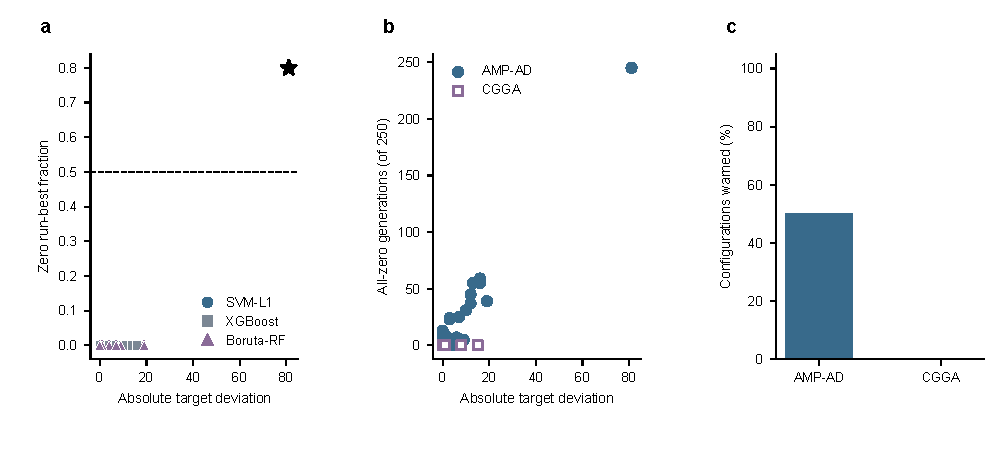
\includegraphics[width=170mm]{v19_work/supplement_polish_20261105/modern/figures/figure_s17.pdf}}
\caption{Original-configuration zero-truncation diagnostics. a) Absolute target-size deviation versus the fraction of zero run-best fitness values. Circles, squares, and triangles denote SVM-L1, XGBoost, and Boruta-RF; the star marks the AMP-AD Rush/SVM-L1/Small failure mode, and the dashed line marks a zero-fraction value of 0.5. b) Absolute target-size deviation versus all-zero generations. Filled blue circles denote AMP-AD and open plum squares denote CGGA. c) Percentage of configurations with a flattening warning in each dataset.}
\label{fig:supp1}
\end{figure}

\begin{figure}[p]
\centering
\makebox[\linewidth][c]{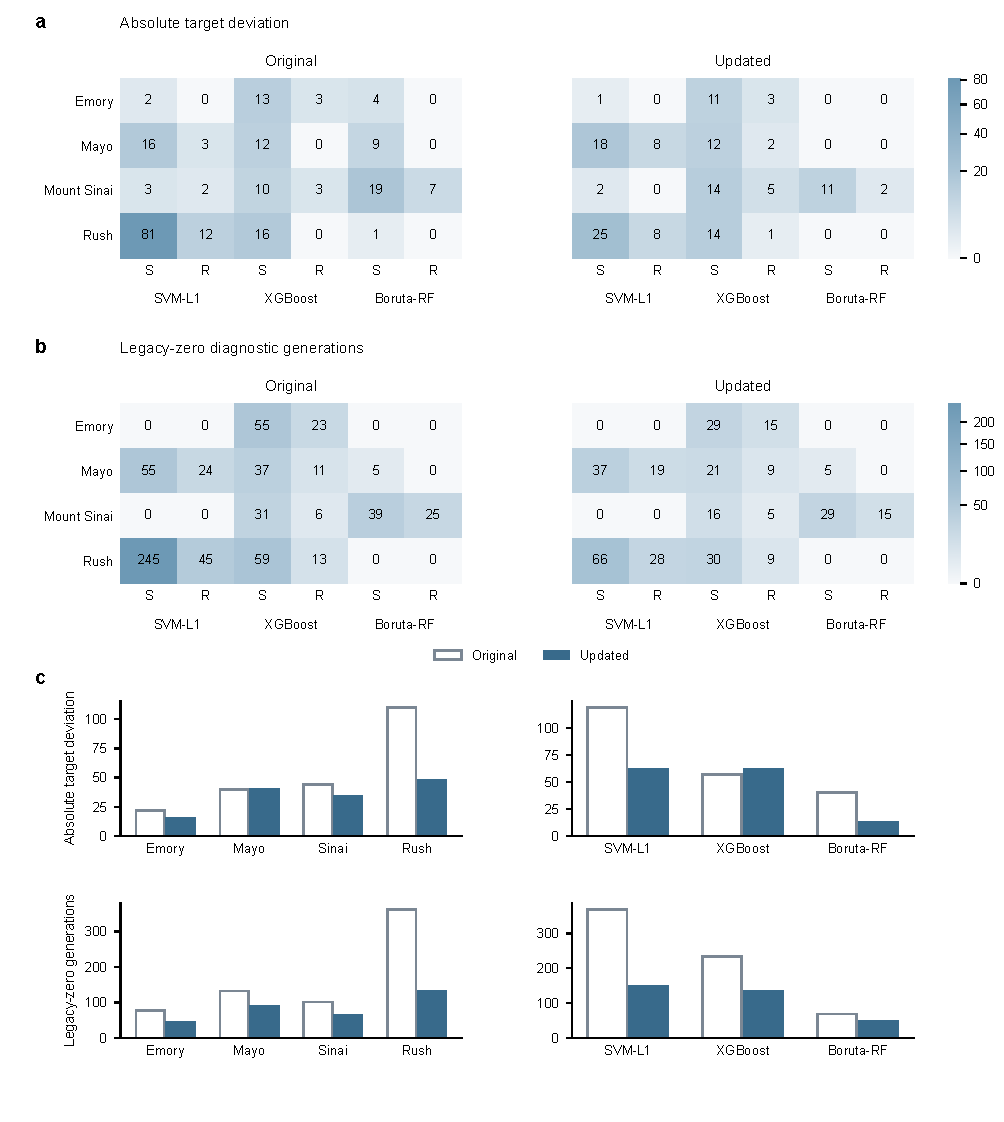
\includegraphics[width=170mm]{v19_work/supplement_polish_20261105/modern/figures/figure_s18.pdf}}
\caption{Complete development-only original-versus-corrected-objective AMP-AD comparison across 24 combinations of center, branch, and cap, using 120 corrected-objective GA runs and matched archived original banks. a) Absolute target deviation. b) Legacy-zero diagnostic generations; corrected-run counts apply the legacy truncation rule to their recorded populations and do not count actual sampling fallbacks. c) Aggregates by center and branch. In a and b, S and R denote Small and Reference caps; Sinai abbreviates Mount Sinai in c. Overall values were 216 versus 137 and 673 versus 333, respectively; detailed robust summaries are in \cref{tab:supp2}. Held-out outcomes were not accessed.}
\label{fig:supp2}
\end{figure}

\begin{figure}[p]
\centering
\makebox[\linewidth][c]{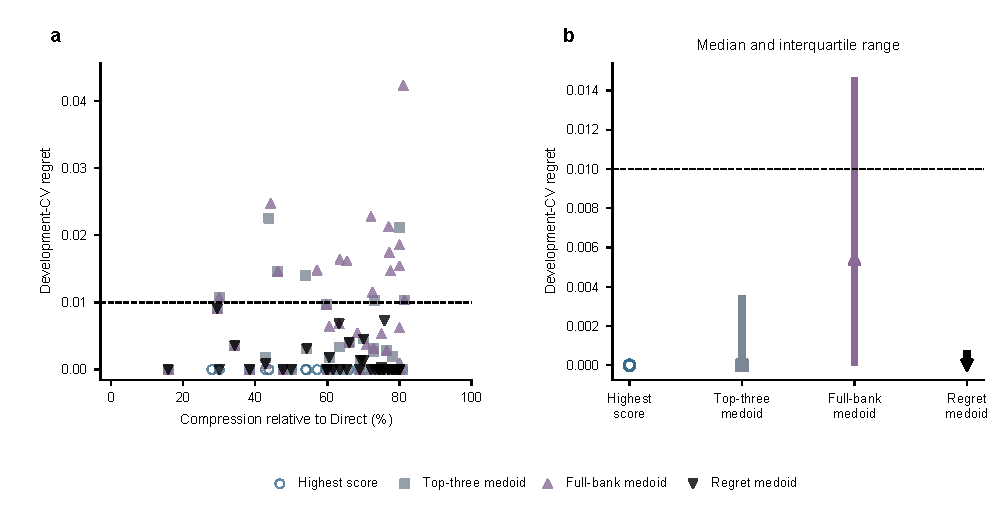
\includegraphics[width=170mm]{v19_work/supplement_polish_20261105/modern/figures/figure_s15.pdf}}
\caption{Development-only compression and regret. a) Compression relative to each Direct candidate set versus development-CV regret for highest-locking-score selection (open circles), the top-three medoid (squares), the unrestricted full-bank medoid (upward triangles), and the regret-constrained medoid at absolute tolerance 0.01 (downward triangles). The dashed line marks the 0.01 empirical-regret bound. b) Median development-CV regret (markers) and interquartile range (vertical bars) by locking rule. Held-out outcomes were not used to define any displayed rule.}
\label{fig:supp3}
\end{figure}

\begin{figure}[p]
\centering
\makebox[\linewidth][c]{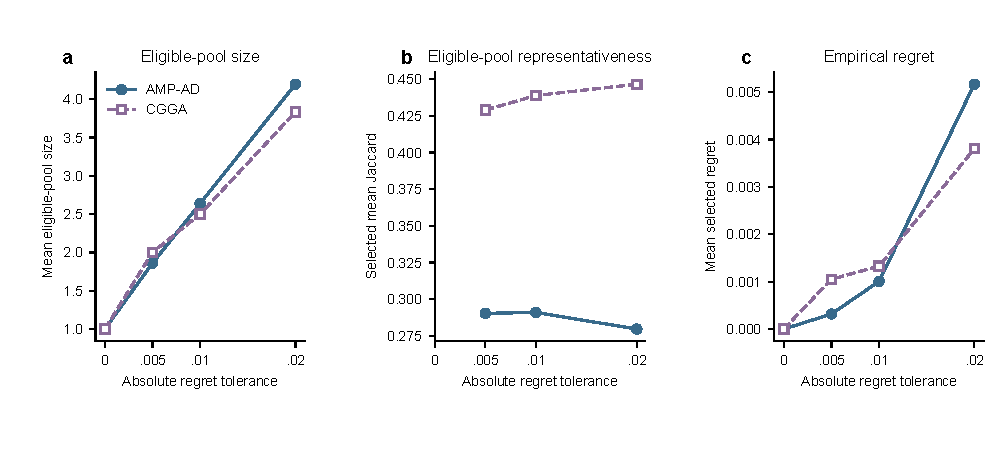
\includegraphics[width=170mm]{v19_work/supplement_polish_20261105/modern/figures/figure_s16.pdf}}
\caption{Development-only strict locking-rule sensitivity. a) Mean eligible-pool size. b) Selected-candidate mean eligible-pool Jaccard for nonsingleton pools; singleton values are undefined and shown as missing. c) Mean selected empirical development-CV regret across absolute tolerances 0, 0.005, 0.01, and 0.02. No tolerance-expanding fallback was used.}
\label{fig:supp4}
\end{figure}

\begin{figure}[p]
\centering
\textit{Supplementary Figure S5. Complete candidate-level audit of fully nested TCGA locking (continued on the next page).}\par\medskip
\makebox[\linewidth][c]{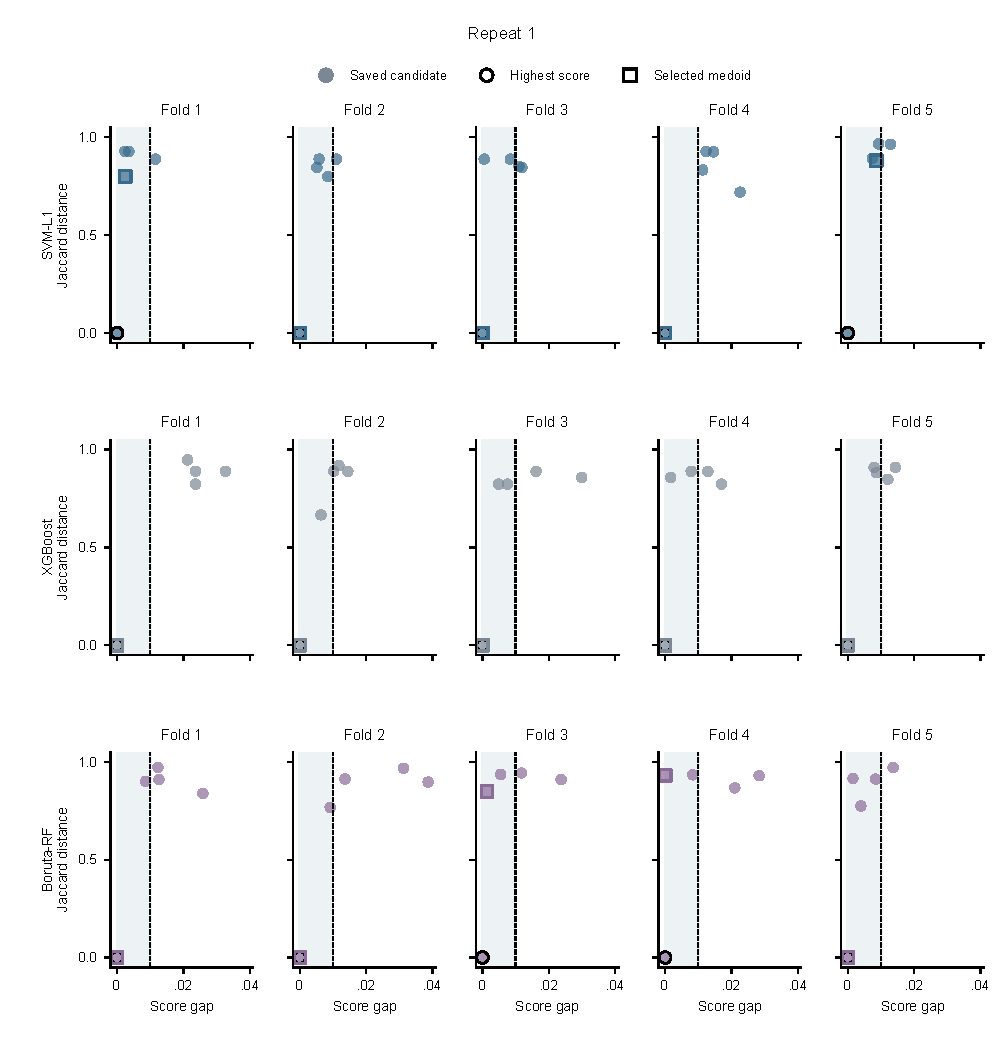
\includegraphics[width=170mm]{v19_work/supplement_polish_20261105/modern/figures/figure_s25_repeat_1.pdf}}
\end{figure}

\begin{figure}[p]
\centering
\makebox[\linewidth][c]{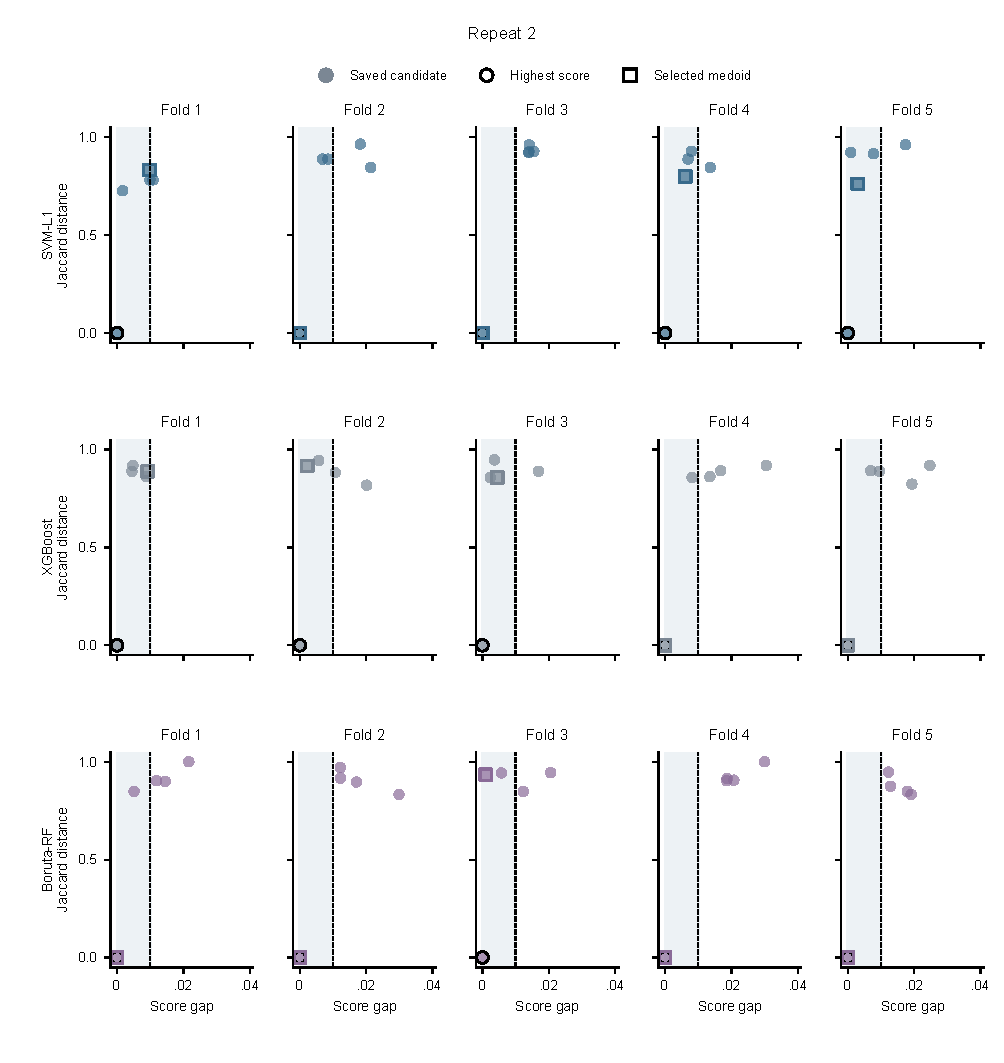
\includegraphics[width=170mm]{v19_work/supplement_polish_20261105/modern/figures/figure_s25_repeat_2.pdf}}
\caption{Complete candidate-level audit of fully nested TCGA locking. The first and second pages show outer repeats 1 and 2, respectively. Each panel represents one branch and outer fold. Points are the five saved GA candidates, positioned by empirical development-CV regret and Jaccard distance from the highest-locking-score mask. Shading denotes the absolute regret-eligible region $R_r\leq0.01$, and dashed lines mark $\delta=0.01$. Open circles identify highest-locking-score candidates and open squares identify selected regret-constrained medoids; markers overlap when the same candidate satisfies both roles. Selection and locking used outer-training data only.}
\label{fig:supp5}
\end{figure}

\begin{figure}[p]
\centering
\makebox[\linewidth][c]{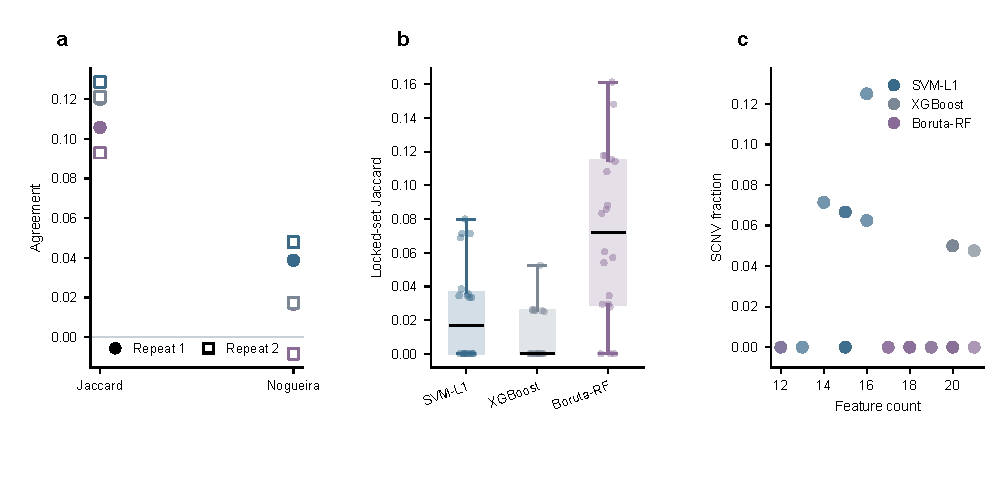
\includegraphics[width=170mm,trim=0mm 10mm 0mm 3mm,clip]{v19_work/supplement_polish_20261105/modern/figures/figure_s26.pdf}}
\caption{Candidate agreement, partition sensitivity, and locked-signature composition in TCGA GBM/LGG. a) Mean pairwise Jaccard and chance-corrected Nogueira stability among five saved candidates. Each point is the unweighted mean of five fold-level bank statistics for one repeat--branch combination and is conditional on each bank's fixed post-Direct universe. Filled circles and open squares denote repeats 1 and 2. The coefficients are shown side by side and are not connected as an effect estimate; a small negative finite-sample Nogueira estimate is valid. b) Jaccard similarity for the 20 dependent outer-fold locked-signature pairs per branch, summarized descriptively. c) Selected feature count and SCNV fraction for each of 30 locked signatures. Eleven of 526 selected-feature occurrences were SCNV features; composition largely reflects upstream Direct screening and is not evidence of biological modality preference. These summaries characterize conditional algorithmic agreement and participant-partition sensitivity, not biomarker stability.}
\label{fig:supp6}
\end{figure}

\begin{figure}[p]
\centering
\makebox[\linewidth][c]{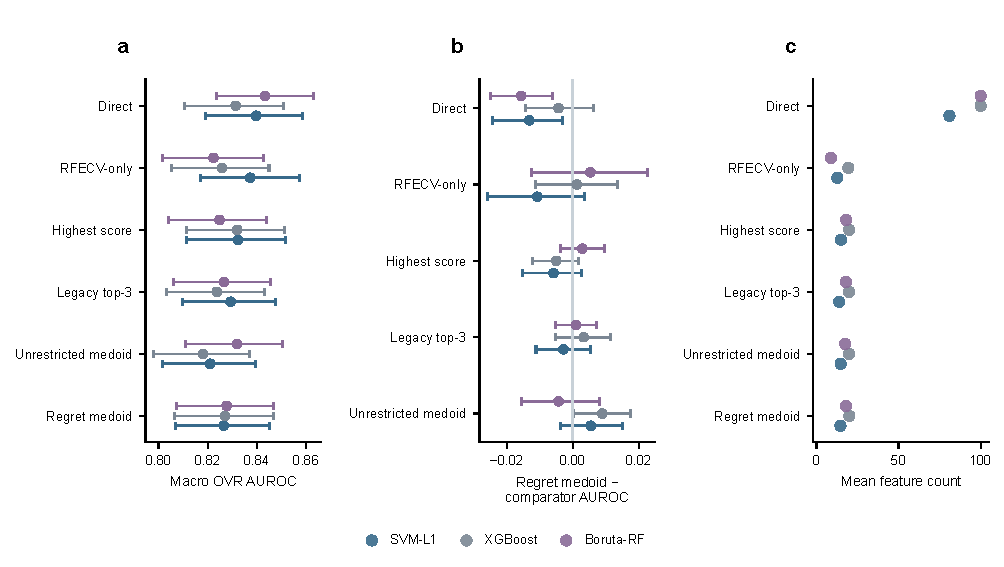
\includegraphics[width=170mm,trim=0mm 2mm 0mm 4mm,clip]{v19_work/supplement_polish_20261105/modern/figures/figure_s27.pdf}}
\caption{Repeated internal out-of-fold comparator audit in TCGA GBM/LGG. a) Mean repeated-OOF macro one-vs-rest AUROC for Direct, RFECV-only, highest-locking-score selection, the top-three medoid, the unrestricted full-bank medoid, and the regret-constrained medoid. b) Paired regret-constrained-medoid-minus-comparator AUROC differences. Points in a) and b) have 95\% participant-clustered, class-stratified bootstrap intervals from 2,000 resamples retaining both repeat-specific predictions for each sampled participant. c) Mean feature count across ten outer folds. The protocol capped each post-Direct universe at 100 features. Colors identify branches. All three regret-constrained-medoid-versus-RFECV-only intervals included zero; equivalence was not tested.}
\label{fig:supp7}
\end{figure}

\begin{figure}[p]
\centering
\makebox[\linewidth][c]{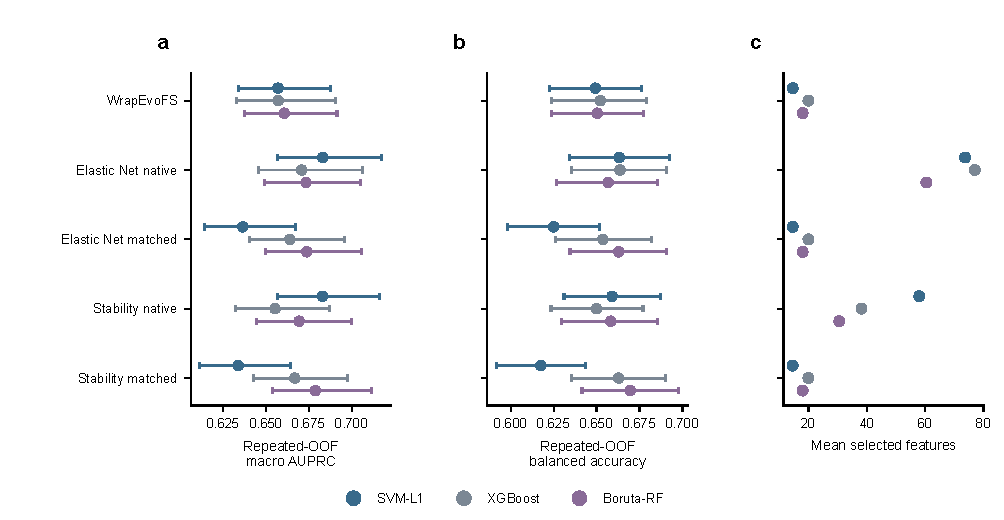
\includegraphics[width=170mm,trim=0mm 1mm 0mm 3mm,clip]{v19_work/supplement_polish_20261105/modern/figures/figure_s_matched_comparator_strengthened.pdf}}
\caption{Extended fully nested TCGA selector-layer sensitivity. a) Repeated-OOF macro AUPRC for regret-constrained-medoid WrapEvoFS, native and cardinality-matched Elastic Net, and native and cardinality-matched subsampling stability selection. b) Balanced accuracy for the same selectors. Points in a) and b) have 95\% participant-clustered, class-stratified bootstrap intervals from 2,000 resamples retaining both repeat-specific predictions for each sampled participant. c) Mean selected-feature counts across ten outer folds. Colors identify Direct branches. Native and matched signatures answer different questions; the matched sets are prespecified cardinality sensitivities, not native nonzero supports. The analysis is conditional on verified post-Direct universes.}
\label{fig:supp8}
\end{figure}

\begin{figure}[p]
\centering
\makebox[\linewidth][c]{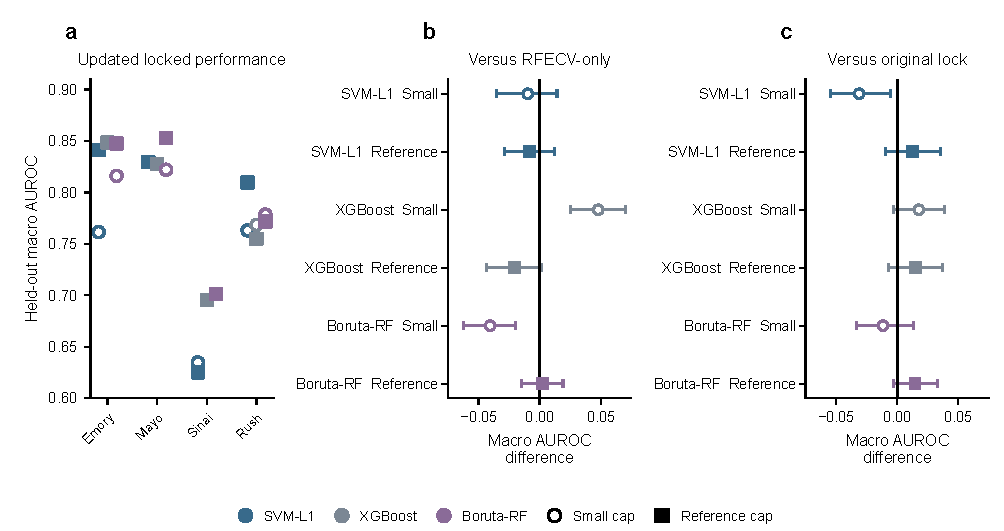
\includegraphics[width=170mm,trim=0mm 0mm 0mm 2mm,clip]{v19_work/supplement_polish_20261105/modern/figures/figure_s21.pdf}}
\caption{AMP-AD one-time post-freeze held-out evaluation of the corrected objective with regret-constrained medoid locking. a) Macro one-vs-rest AUROC for 24 frozen signatures across combinations of center, branch, and cap; colors identify branches, open circles denote the Small cap, and filled squares denote the Reference cap. Sinai abbreviates Mount Sinai. b) Pooled regret-constrained-medoid-minus-RFECV-only and c) regret-constrained-medoid-minus-top-three medoid macro-AUROC differences with 95\% intervals from 2,000 common resamples stratified by held-out center and true class (seed 42). All masks, parameters, and the protocol hash were frozen before held-out outcomes were loaded; evaluation triggered no reselection or parameter changes. Four of six intervals in b) and five of six in c) include zero.}
\label{fig:supp9}
\end{figure}

\begin{figure}[p]
\centering
\makebox[\linewidth][c]{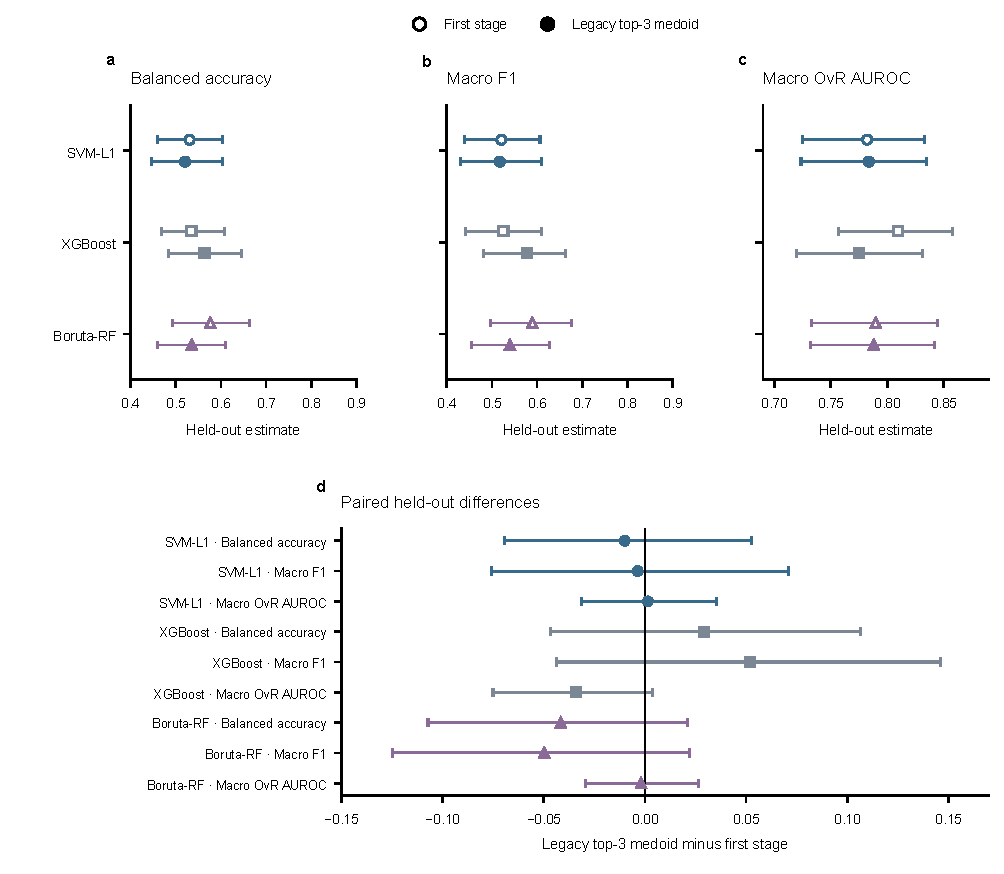
\includegraphics[width=170mm]{figures/supp_polished/supp_s10.pdf}}
\caption{ADNI held-out performance and paired differences. a) Balanced accuracy, b) macro F1, and c) macro one-vs-rest AUROC for the first-stage Direct signatures (open symbols) and archived top-three medoid signatures (filled symbols), shown by branch with 95\% bootstrap confidence intervals. d) Paired top-three medoid-minus-first-stage differences from 5,000 class-stratified paired bootstrap resamples. All nine paired 95\% confidence intervals include zero; equivalence and non-inferiority were not tested.}
\label{fig:supp10}
\end{figure}

\begin{figure}[p]
\centering
\makebox[\linewidth][c]{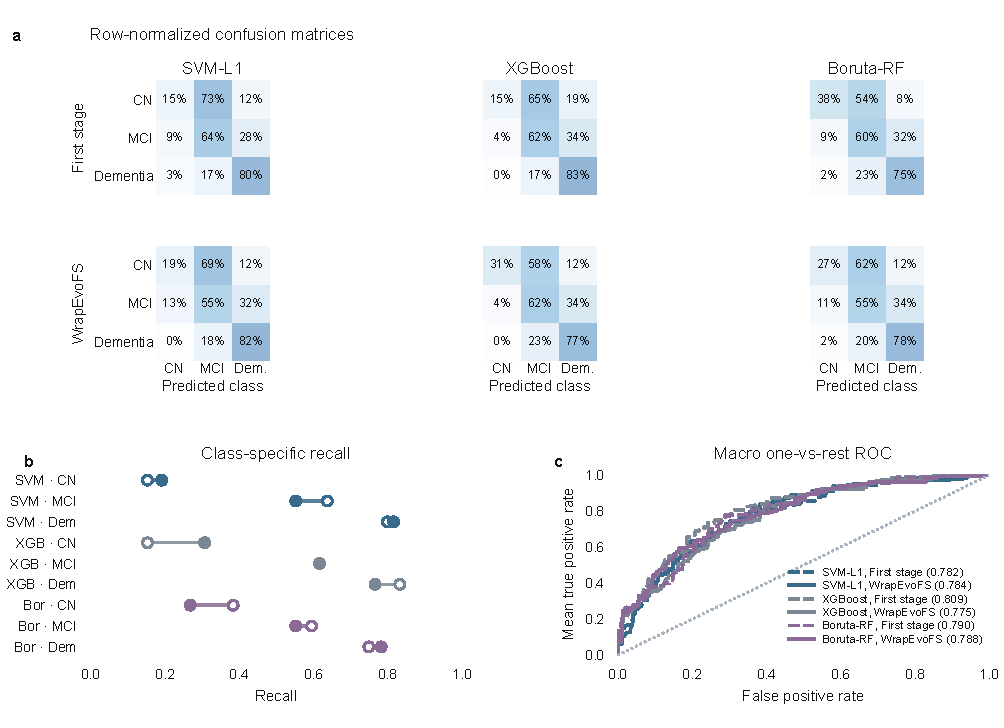
\includegraphics[width=170mm]{figures/supp_polished/supp_s11.pdf}}
\caption{ADNI multiclass held-out diagnostics. a) Row-normalized confusion matrices for the first-stage Direct and archived top-three medoid signatures in the SVM-L1, XGBoost, and Boruta-RF branches. b) Class-specific recall for CN, MCI, and dementia, with open and filled symbols denoting first-stage and archived top-three medoid signatures, respectively. c) Macro one-vs-rest ROC curves and AUROC values for the same six models.}
\label{fig:supp11}
\end{figure}

\begin{figure}[p]
\centering
\makebox[\linewidth][c]{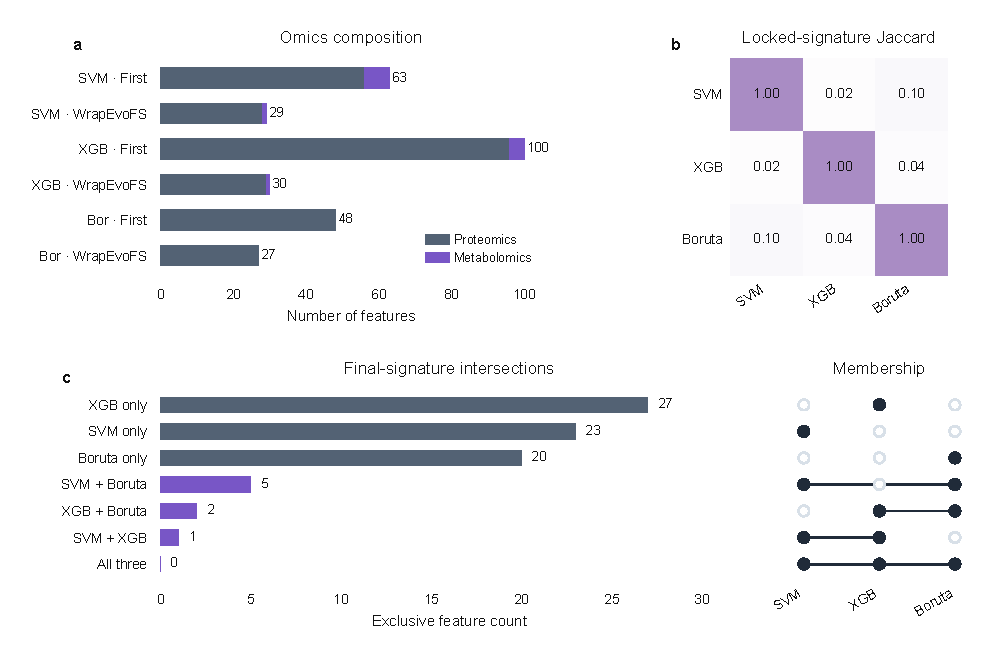
\includegraphics[width=170mm]{figures/supp_polished/supp_s12.pdf}}
\caption{ADNI signature composition and cross-branch overlap. a) Proteomic and metabolomic feature counts for first-stage and archived top-three medoid signatures in each branch. b) Pairwise Jaccard similarity among the three locked signatures. c) Exclusive and shared locked-signature feature counts shown with an intersection-membership matrix. The displayed sets are descriptive and are not stable biomarker claims.}
\label{fig:supp12}
\end{figure}

\begin{figure}[p]
\centering
\makebox[\linewidth][c]{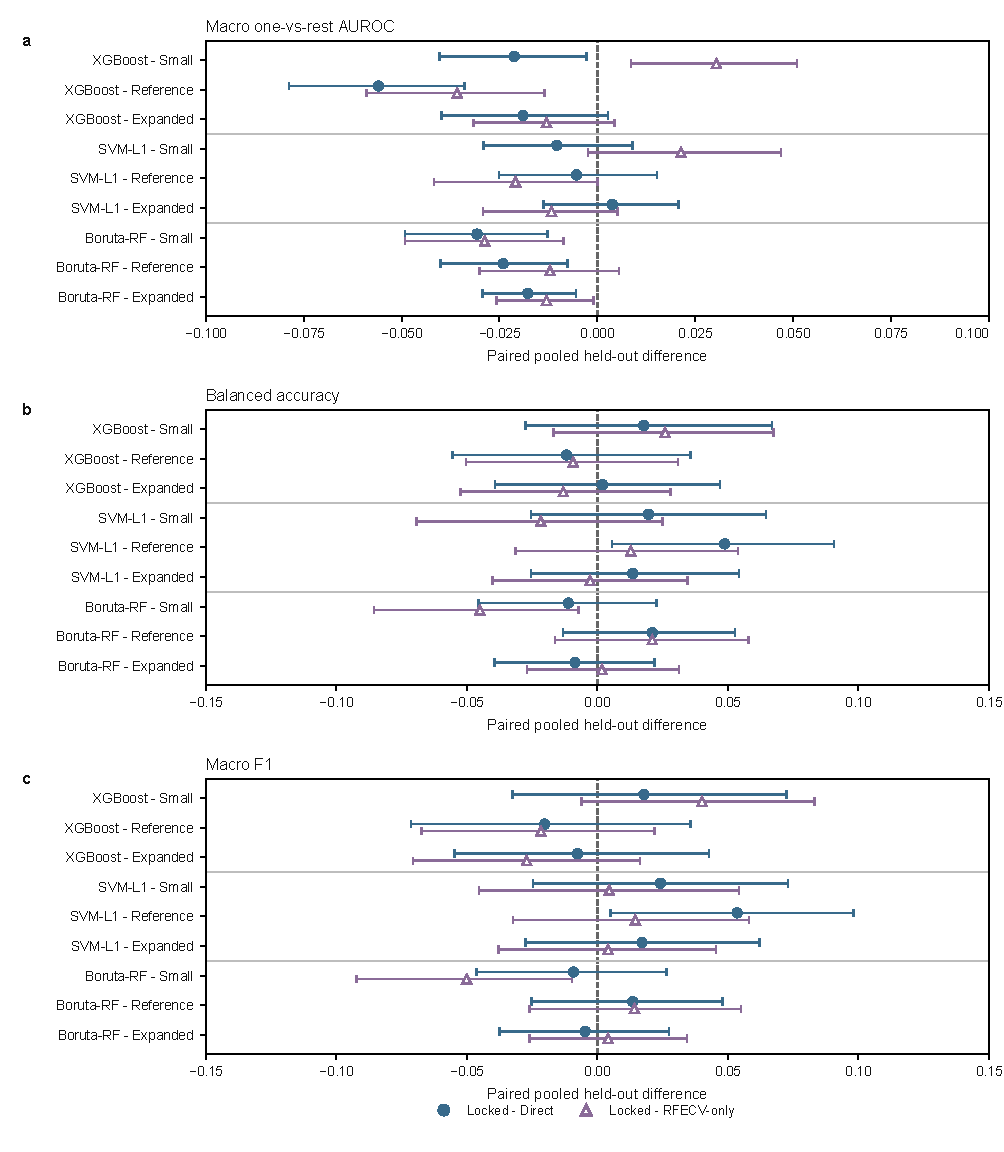
\includegraphics[width=170mm]{figures/supp_polished/supp_s13.pdf}}
\caption{AMP-AD paired pooled held-out differences across RFECV cap settings. a) Macro one-vs-rest AUROC, b) balanced accuracy, and c) macro F1. Filled circles show locked-minus-Direct differences and open triangles show locked-minus-RFECV-only differences; horizontal intervals are 95\% paired confidence intervals. Forty of 54 exported intervals include zero; directions vary by branch, cap, metric, and comparator, and resampling conditions on four fitted center-specific models.}
\label{fig:supp13}
\end{figure}

\begin{figure}[p]
\centering
\makebox[\linewidth][c]{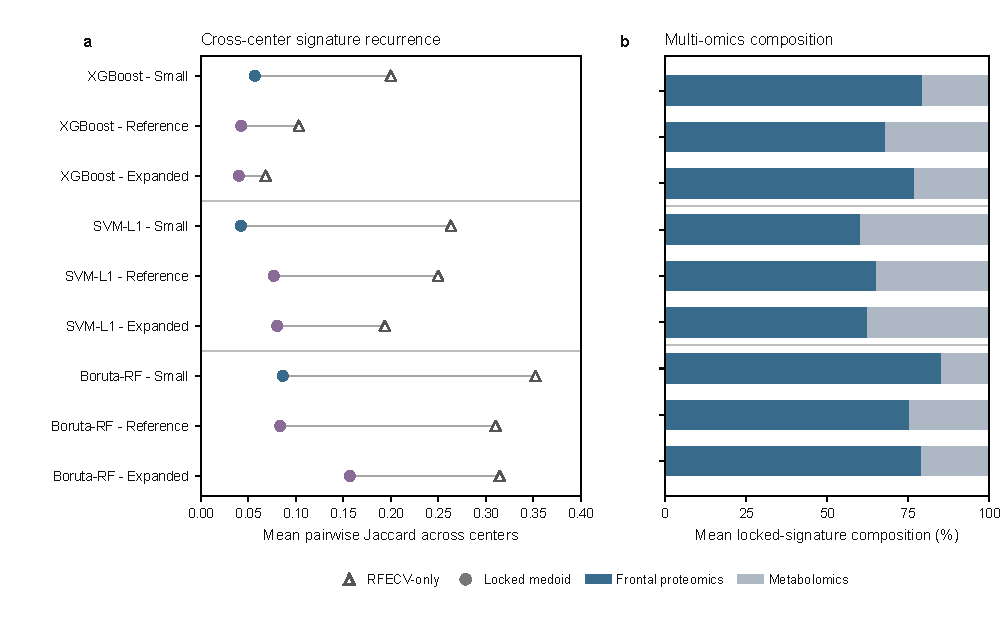
\includegraphics[width=170mm]{figures/supp_polished/supp_s14.pdf}}
\caption{AMP-AD cross-center recurrence and modality composition. a) Mean pairwise Jaccard similarity across centers for RFECV-only and archived top-three medoid signatures in each branch and cap condition. b) Mean locked-signature composition split between frontal proteomics and metabolomics for the same conditions. Cross-center overlap quantifies recurrence across center-specific training sets, not biological replication.}
\label{fig:supp14}
\end{figure}

\begin{figure}[p]
\centering
\makebox[\linewidth][c]{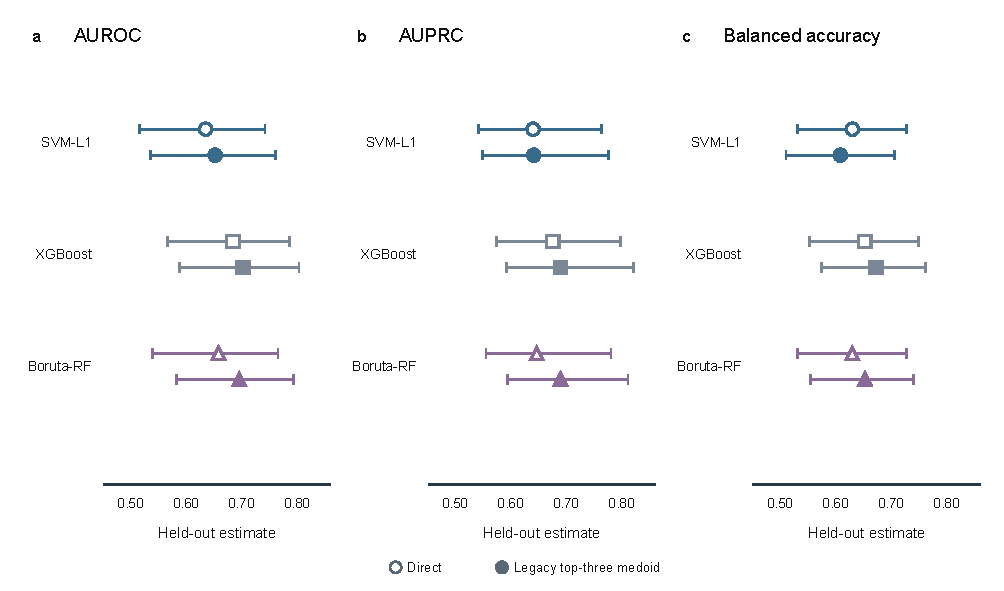
\includegraphics[width=170mm]{figures/supp_polished/supp_s15.pdf}}
\caption{Complete CGGA held-out comparison. a) AUROC, b) AUPRC, and c) balanced accuracy for the Direct signatures (open symbols) and top-three medoid signatures (filled symbols) in the SVM-L1, XGBoost, and Boruta-RF branches; horizontal intervals are the corresponding held-out uncertainty intervals.}
\label{fig:supp15}
\end{figure}

\begin{figure}[p]
\centering
\textit{Supplementary Figure S16. CGGA run-level stochastic agreement (continued on the next page).}\par\medskip
\makebox[\linewidth][c]{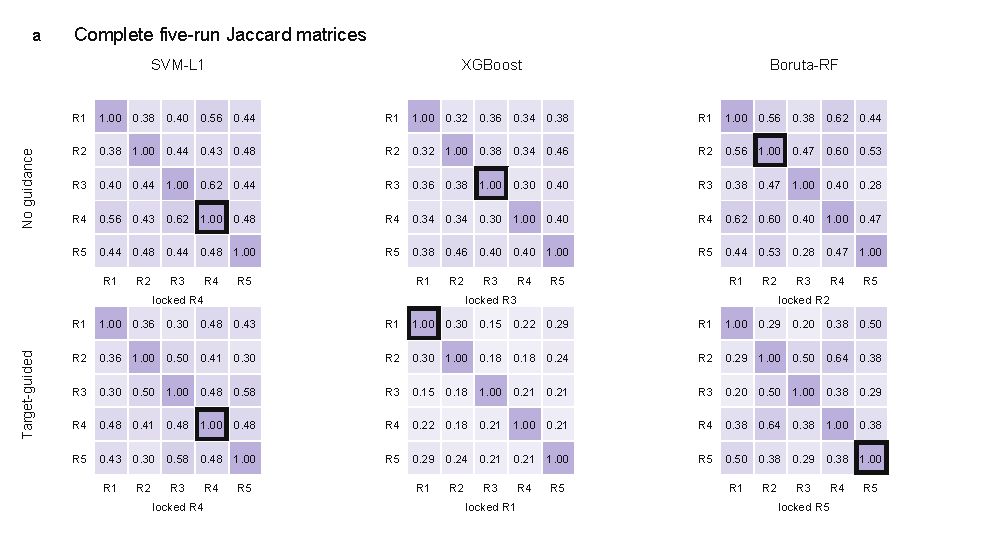
\includegraphics[width=170mm]{figures/supp_polished/supp_s16_a.pdf}}
\end{figure}

\begin{figure}[p]
\centering
\makebox[\linewidth][c]{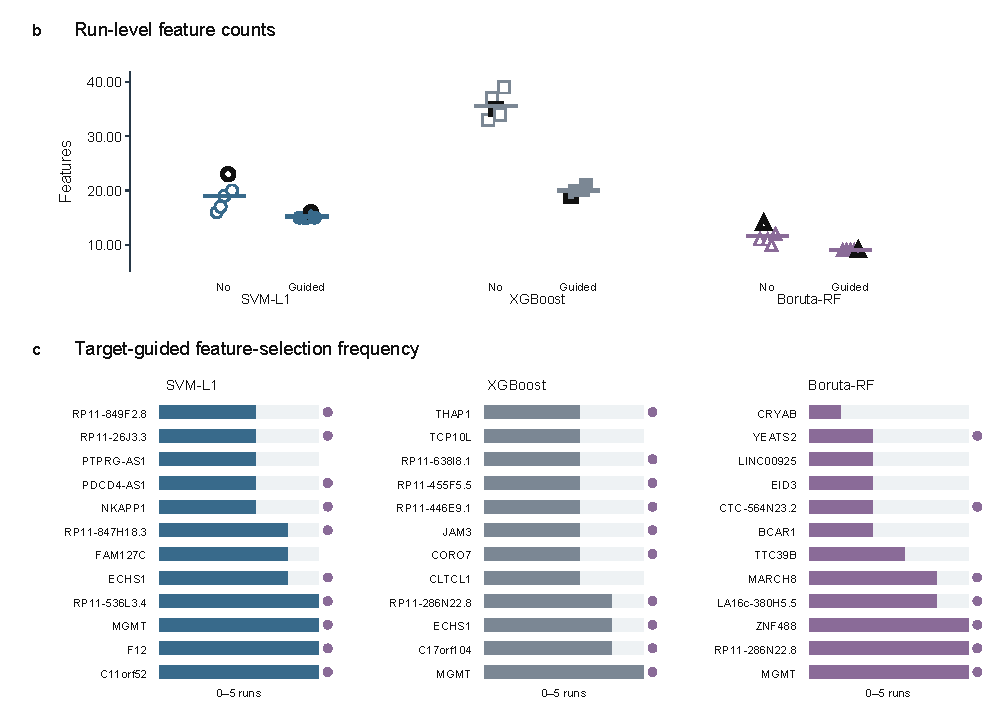
\includegraphics[width=170mm]{figures/supp_polished/supp_s16_bc.pdf}}
\caption{CGGA run-level stochastic agreement. a) Five-run Jaccard matrices without and with target-size guidance; black outlines mark the selected top-three medoid run in a and b. b) Run-level feature counts without and with guidance. c) Target-guided selection frequencies; filled dots mark the top-three medoid signature.}
\label{fig:supp16}
\end{figure}

\begin{figure}[p]
\centering
\textit{Supplementary Figure S17. CGGA original-configuration mechanism and seed-agreement analysis (continued on the next page).}\par\medskip
\makebox[\linewidth][c]{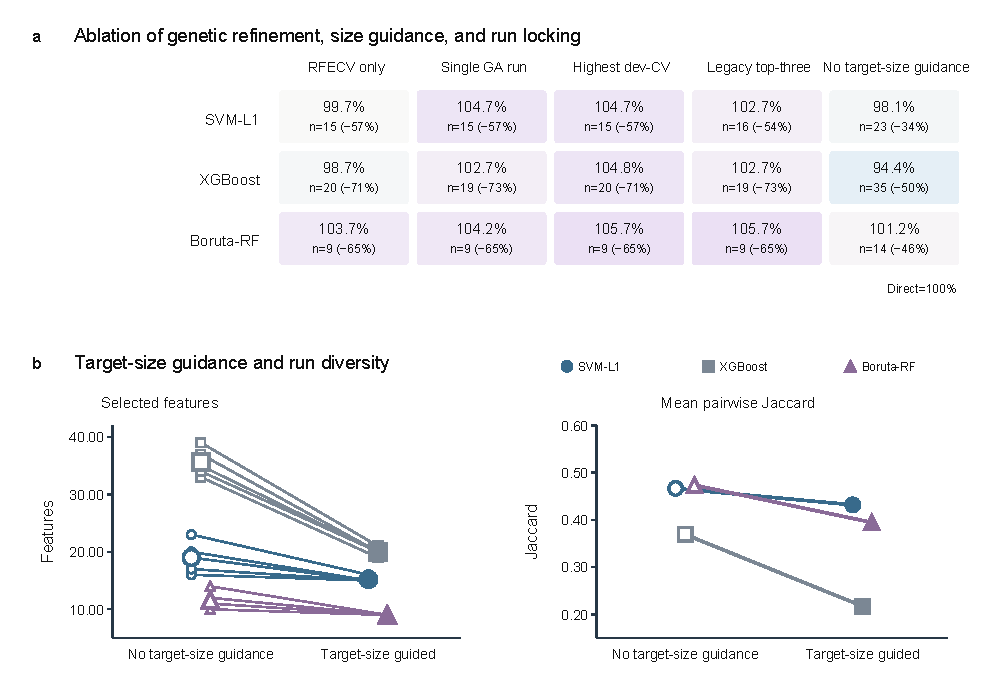
\includegraphics[width=170mm]{figures/supp_polished/supp_s17_ab.pdf}}
\end{figure}

\begin{figure}[p]
\centering
\makebox[\linewidth][c]{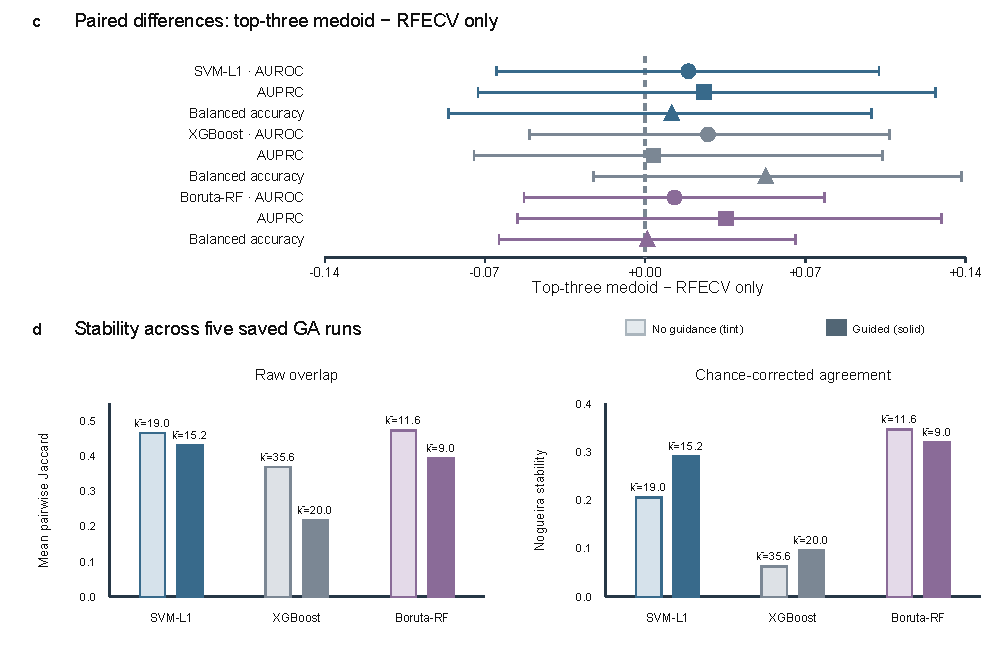
\includegraphics[width=170mm]{figures/supp_polished/supp_s17_cd.pdf}}
\caption{CGGA original-configuration mechanism and seed-agreement ablation. a) Held-out AUROC relative to Direct for RFECV-only and selected-run variants. Cells show the AUROC/Direct ratio, feature count, and feature reduction. The single GA run is prespecified run 1; no guidance sets $\lambda=0$, with the stored target inactive in GA fitness. b) Five-run feature counts and mean pairwise Jaccard with and without target-size guidance. c) Paired top-three medoid-minus-RFECV-only differences. d) Raw Jaccard and chance-corrected Nogueira agreement.}
\label{fig:supp17}
\end{figure}

\begin{figure}[p]
\centering
\makebox[\linewidth][c]{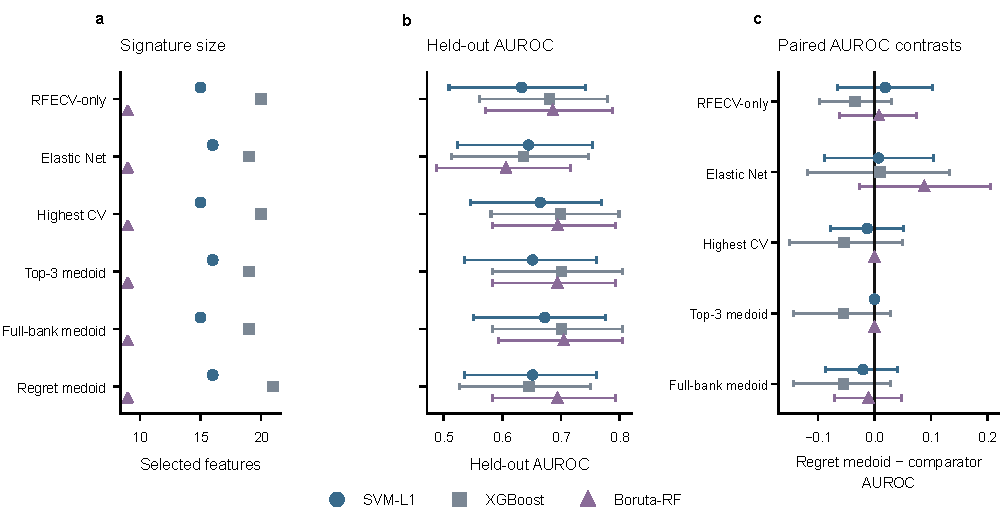
\includegraphics[width=170mm]{figures/supp_polished/supp_s18.pdf}}
\caption{CGGA coherent same-split, same-estimator benchmark. a) Feature counts and b) held-out AUROC with 95\% class-stratified bootstrap intervals for six development-derived signatures in each branch. c) Paired regret-constrained-medoid-minus-comparator AUROC differences from 2,000 common resamples (seed 42); all 15 intervals include zero. All signatures were evaluated with the same fixed 500-tree random forest on the same 92-sample held-out partition. Held-out outcomes did not determine any feature set, locking rule, or comparator.}
\label{fig:supp18}
\end{figure}

\begin{figure}[p]
\centering
\makebox[\linewidth][c]{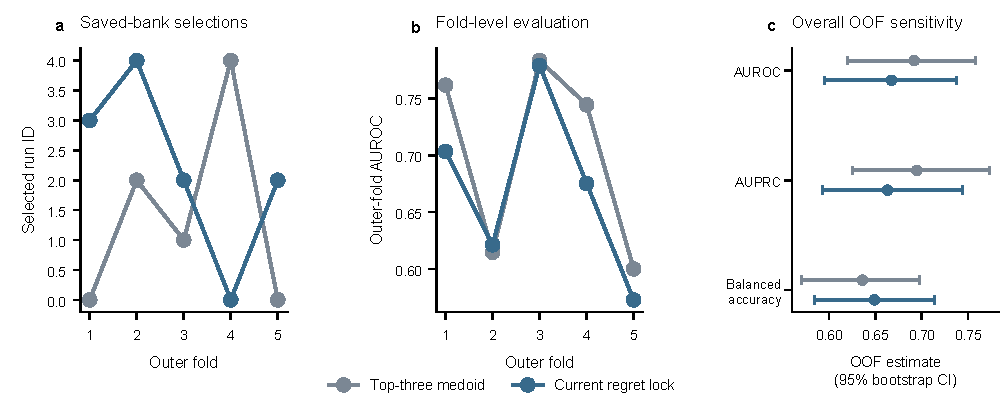
\includegraphics[width=170mm]{figures/supp_polished/supp_s19.pdf}}
\caption{CGGA post hoc saved-bank nested sensitivity. a) Selected run IDs under the top-three medoid and regret-constrained medoid across five outer folds. b) Corresponding outer-fold AUROC. c) Overall OOF AUROC, AUPRC, and balanced accuracy with 95\% class-stratified bootstrap intervals. The regret-constrained medoid changed all five selected runs; OOF AUROC was 0.692 under the top-three medoid and 0.667 under the regret-constrained medoid. The source banks used a reduced historical search budget (20 individuals, 12 generations, five runs), no GA was rerun, and the original 92-sample held-out partition was not accessed.}
\label{fig:supp19}
\end{figure}

\begin{figure}[p]
\centering
\makebox[\linewidth][c]{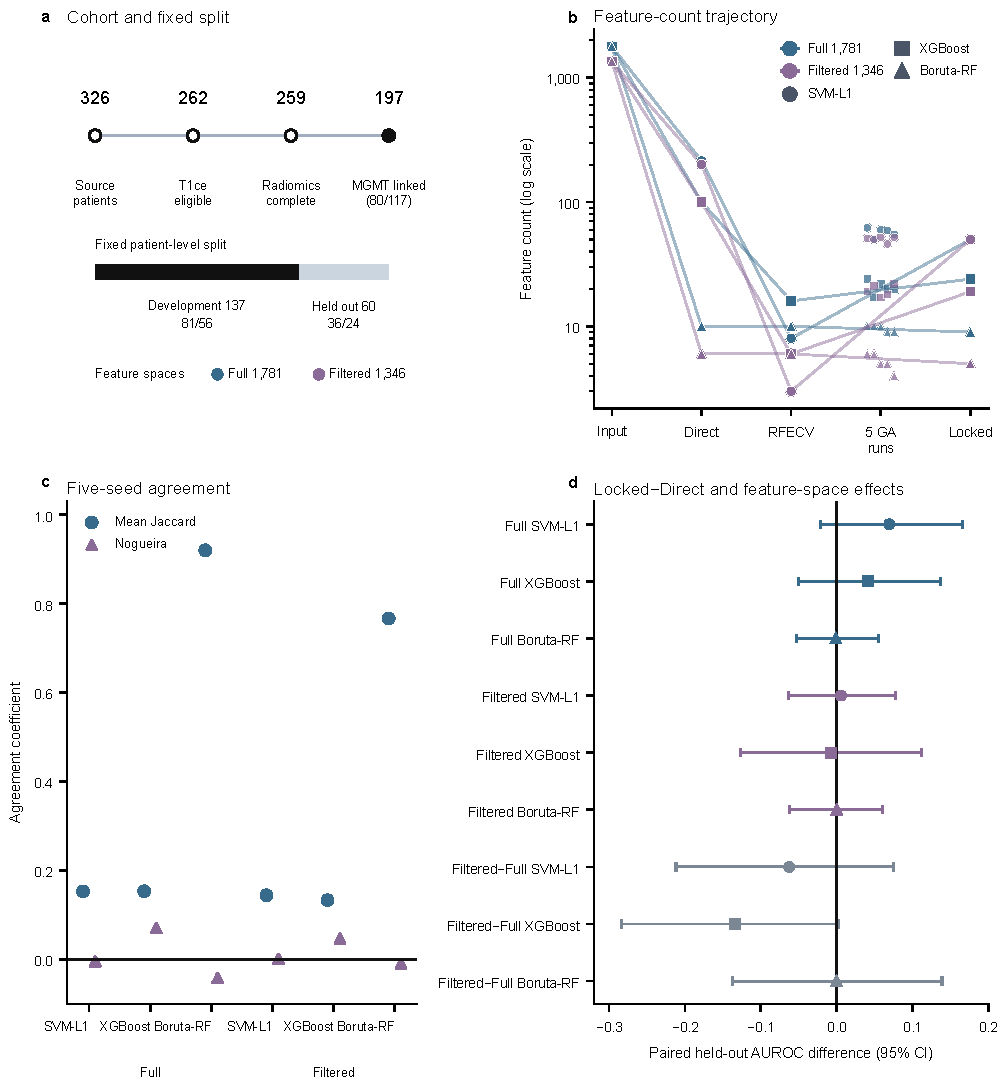
\includegraphics[width=170mm]{figures/supp_polished/supp_s20.pdf}}
\caption{VGH brain-tumour radiomics internal demonstration (UBC REB H20-02354) using regret-constrained locking. a) Cohort reduction, validated MGMT linkage, fixed development/held-out split, and the full and perturbation-filtered feature spaces. b) Feature counts through Direct screening, RFECV target estimation, five completed GA runs, and strict regret-constrained locking. c) Mean pairwise Jaccard and chance-corrected Nogueira agreement across five seeds. d) Paired held-out AUROC differences for locked-minus-Direct and perturbation-filtered-minus-full locked signatures, with 95\% class-stratified bootstrap intervals. Both feature spaces use the same 197 participants and split; the filtered-space contrast is a label-independent feature-definition sensitivity analysis, not external validation. All paired intervals include zero. Five-seed summaries do not estimate participant-resampling or biomarker stability, and automatic tumor-core regions were not manually adjudicated.}
\label{fig:supp20}
\end{figure}

\begin{figure}[p]
\centering
\makebox[\linewidth][c]{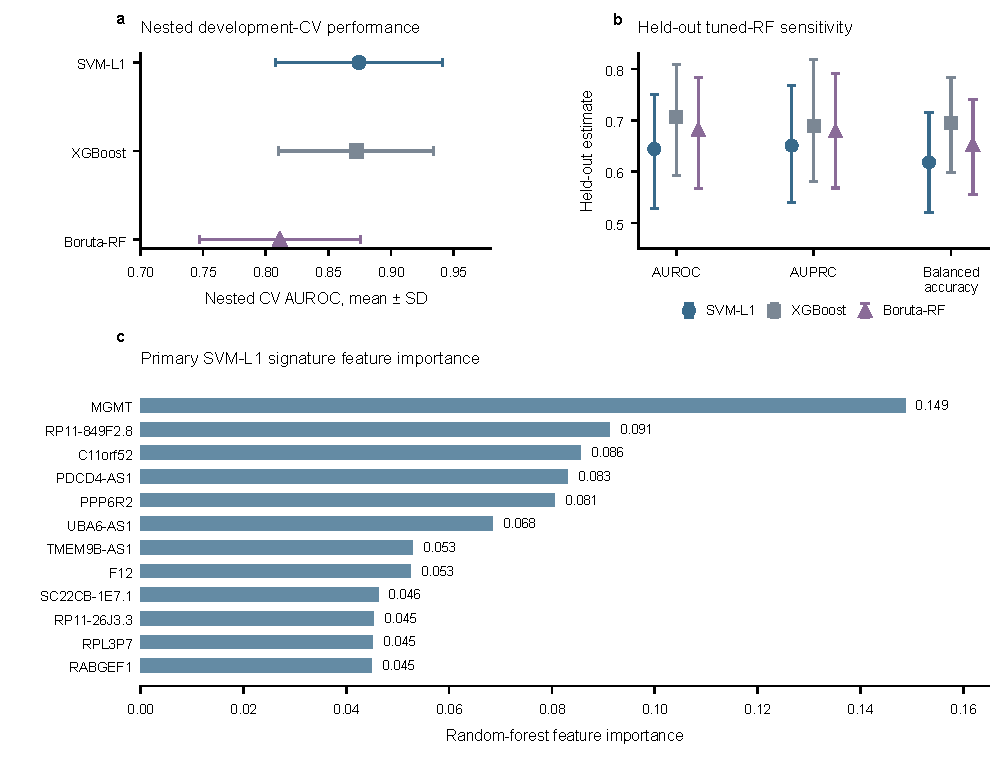
\includegraphics[width=170mm]{figures/supp_polished/supp_s21.pdf}}
\caption{Secondary tuned-random-forest sensitivity. a) Nested development-CV AUROC for the three branches, with the prespecified primary branch identified. b) Held-out tuned-random-forest AUROC, AUPRC, and balanced accuracy with uncertainty intervals. c) Random-forest importance values for the primary SVM-L1 signature. This analysis is descriptive and is not used to support a core claim.}
\label{fig:supp21}
\end{figure}

\begin{figure}[p]
\centering
\makebox[\linewidth][c]{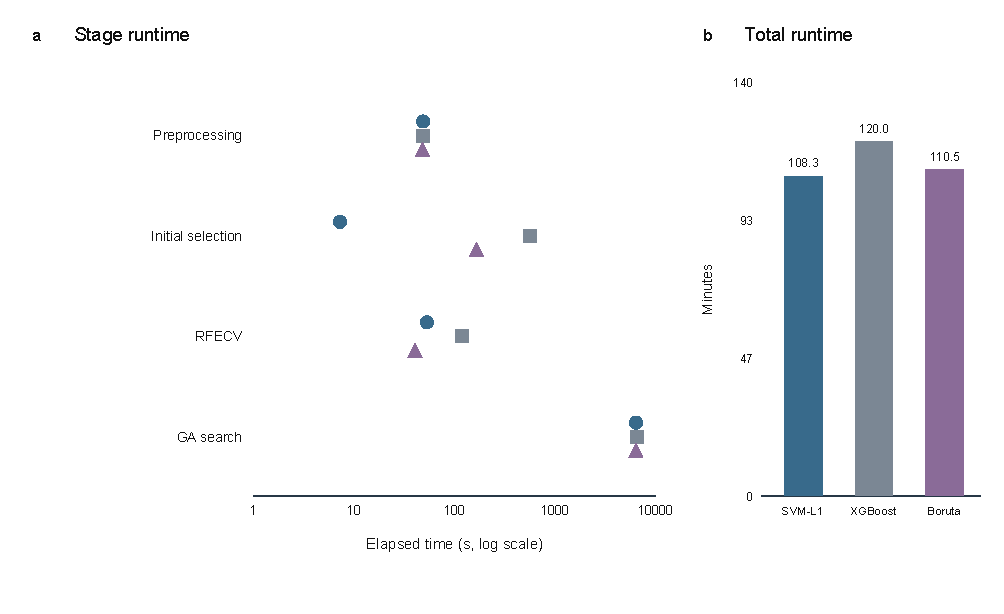
\includegraphics[width=170mm]{figures/supp_polished/supp_s22.pdf}}
\caption{CGGA computational characterization. a) Elapsed time for preprocessing, initial selection, RFECV, and GA search by branch on a logarithmic scale. b) Total runtime by branch. Secondary-analysis peak memory was 178.0 MB; complete runtime and peak-memory values are retained in the machine-readable computational audit.}
\label{fig:supp22}
\end{figure}

\begin{figure}[p]
\centering
\makebox[\linewidth][c]{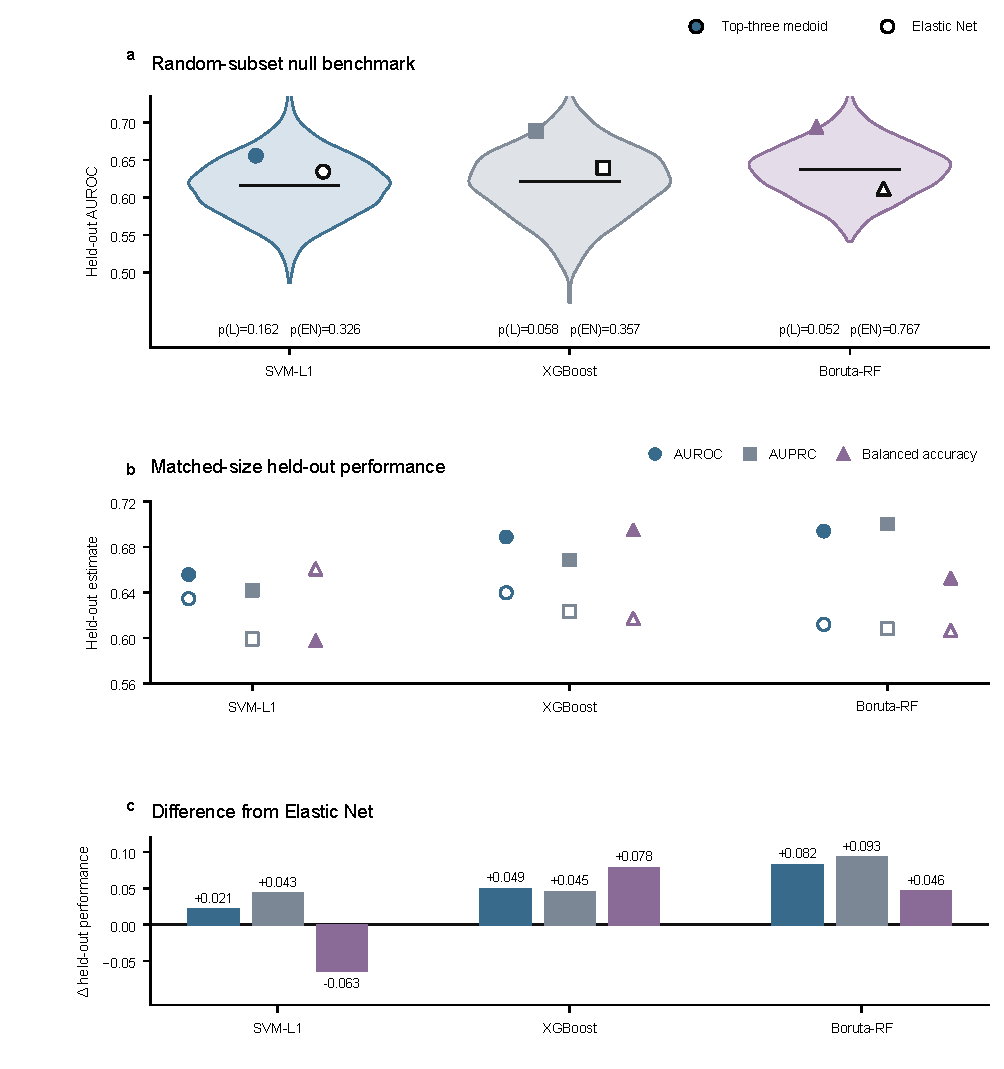
\includegraphics[width=170mm]{figures/supp_polished/supp_s23.pdf}}
\caption{Exploratory CGGA comparators. a) Size-matched random-subset null distributions with the top-three medoid and Elastic Net estimates overlaid (filled and open symbols). The labels p(L) and p(EN) give the respective empirical upper-tail probabilities. b) Matched-size held-out AUROC, AUPRC, and balanced accuracy for the top-three medoid and Elastic Net. c) Top-three medoid-minus-Elastic Net differences for the same three metrics. One-sided empirical random-subset tail probabilities were not multiplicity adjusted, and all paired intervals include zero.}
\label{fig:supp23}
\end{figure}

\begin{figure}[p]
\centering
\makebox[\linewidth][c]{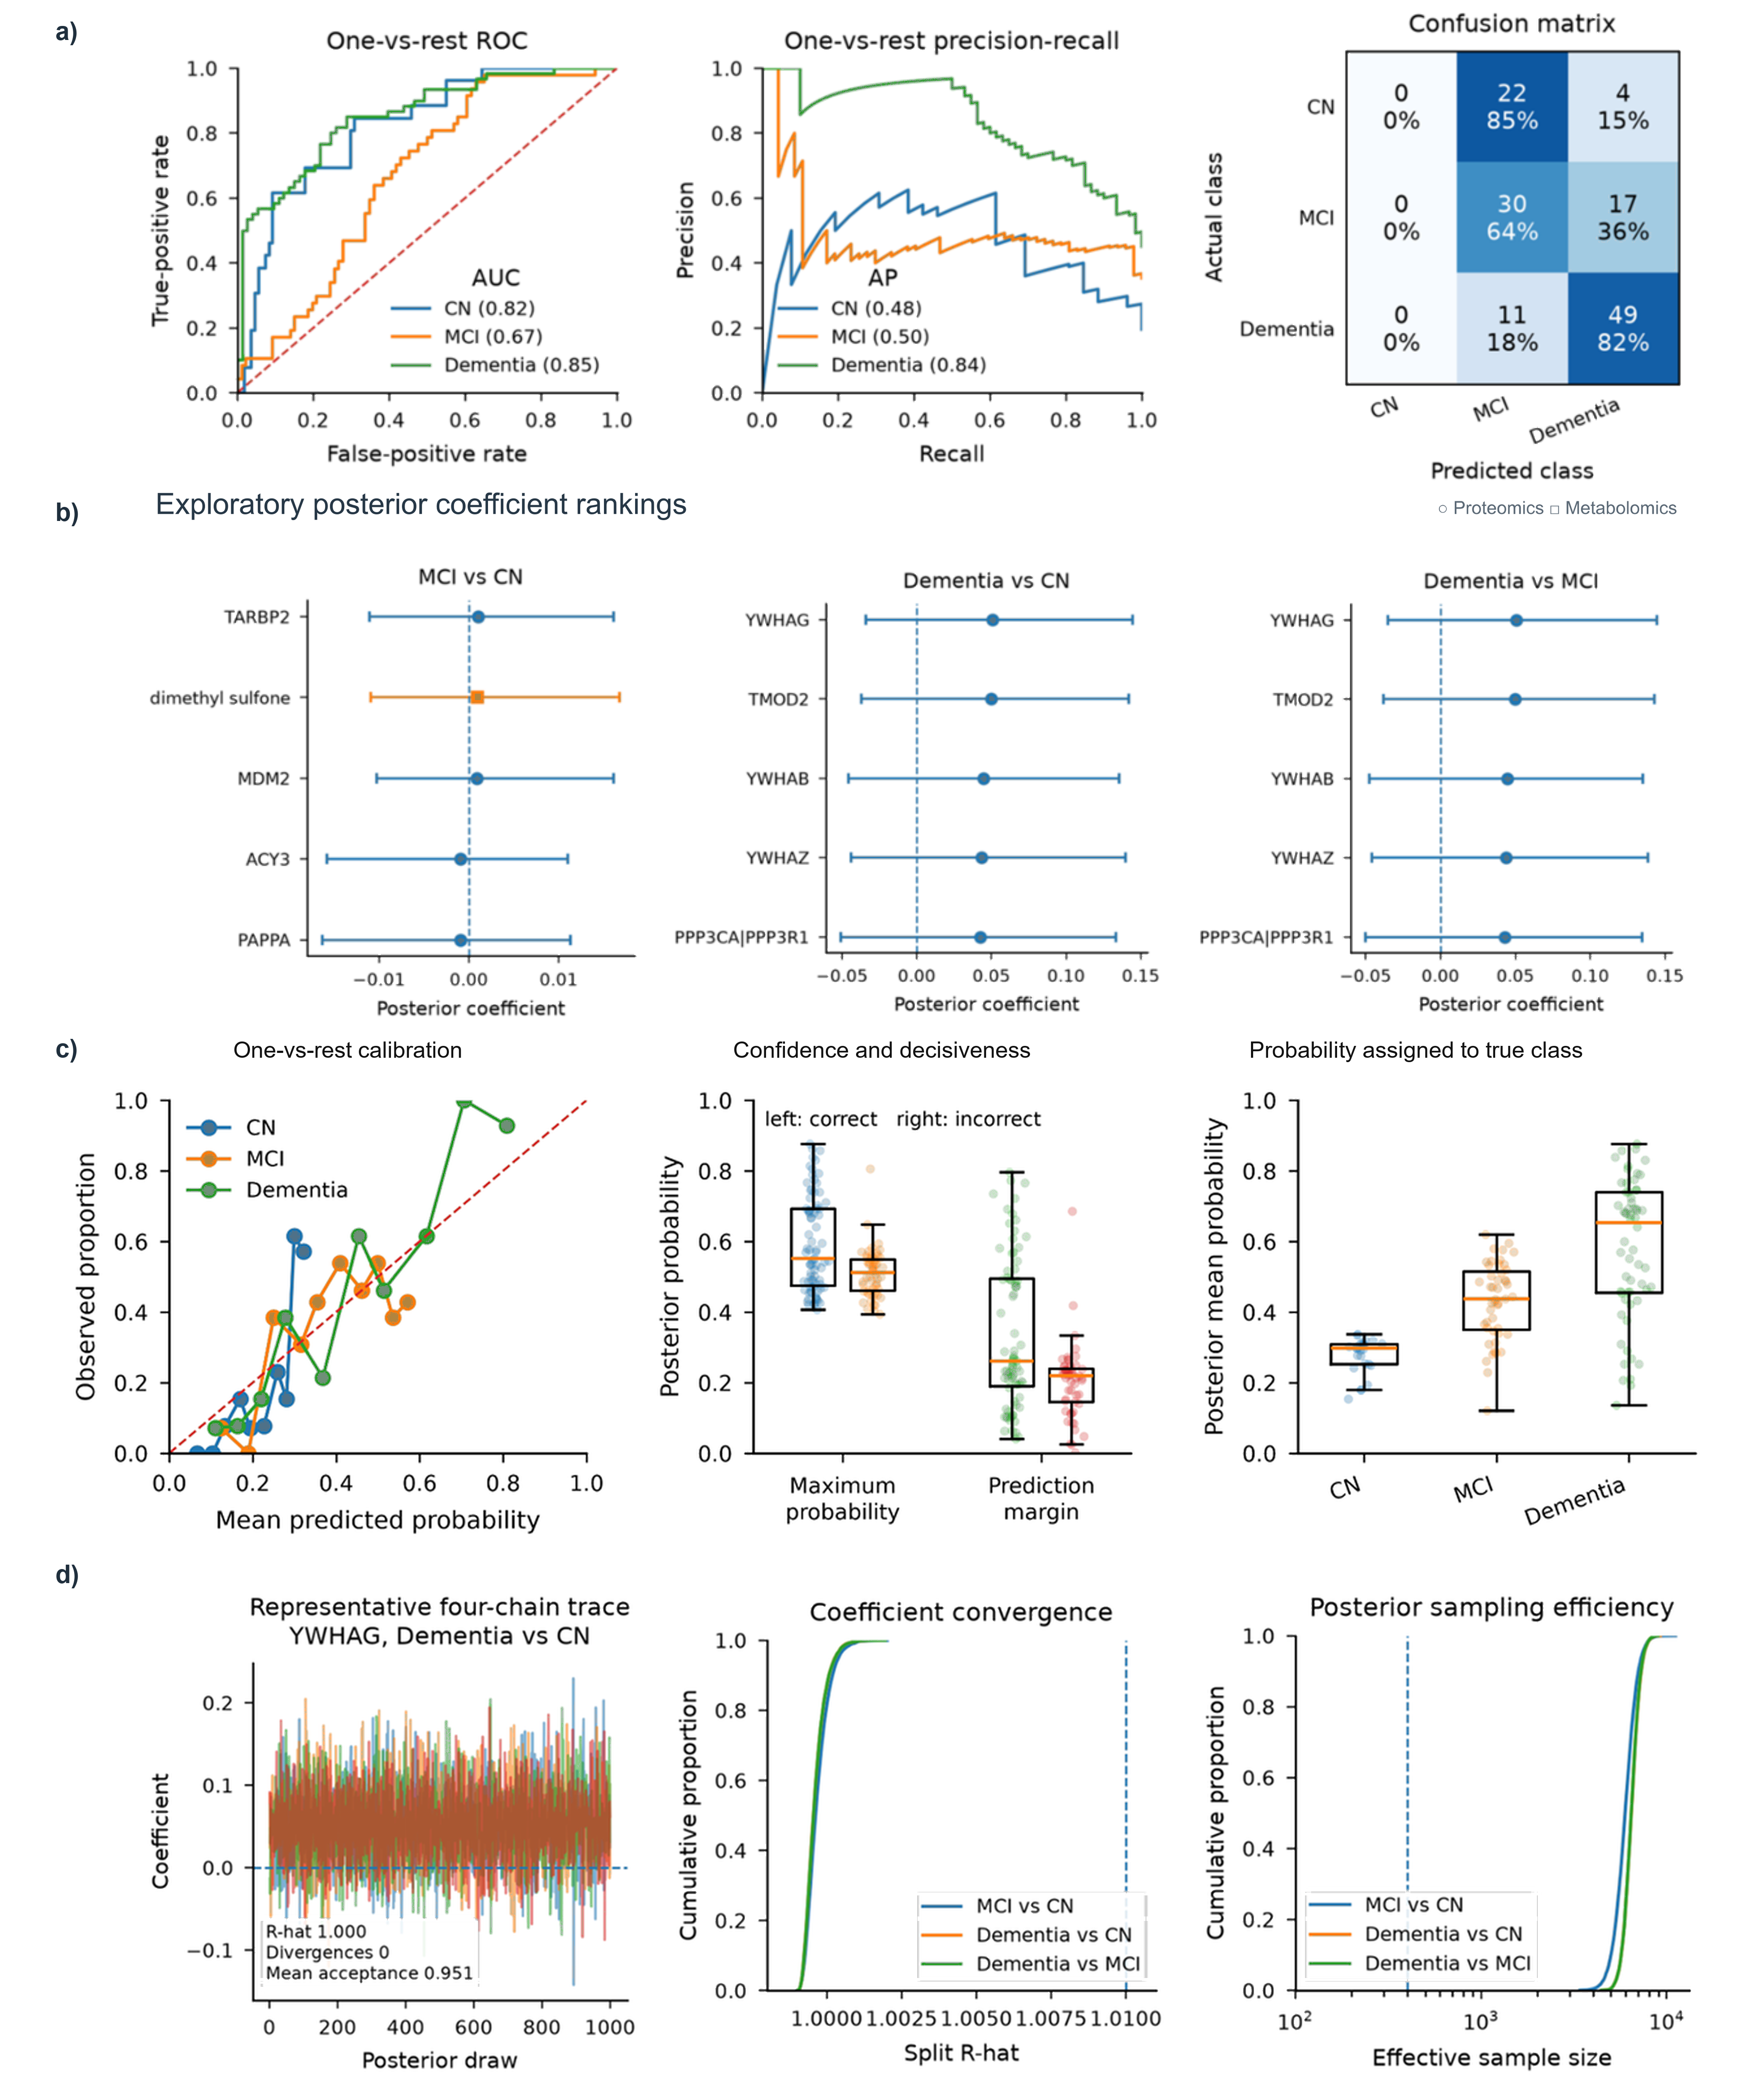
\includegraphics[width=170mm,height=0.78\textheight,keepaspectratio]{figures/figure_s4.png}}
\caption{Full-feature Bayesian predictive reference. a) One-vs-rest ROC and precision-recall curves together with the row-normalized confusion matrix. b) Exploratory posterior coefficient rankings for the three dementia contrasts; points show posterior means and intervals show 95\% credible intervals. c) One-vs-rest calibration, confidence and prediction-margin distributions, and posterior probability assigned to the true class. d) A representative four-chain coefficient trace, the empirical distribution of split R-hat values, and bulk effective sample sizes. Posterior probability rankings retained discrimination while coefficient-level intervals reflected diffuse high-dimensional uncertainty.}
\label{fig:supp24}
\end{figure}

\begin{figure}[p]
\centering
\makebox[\linewidth][c]{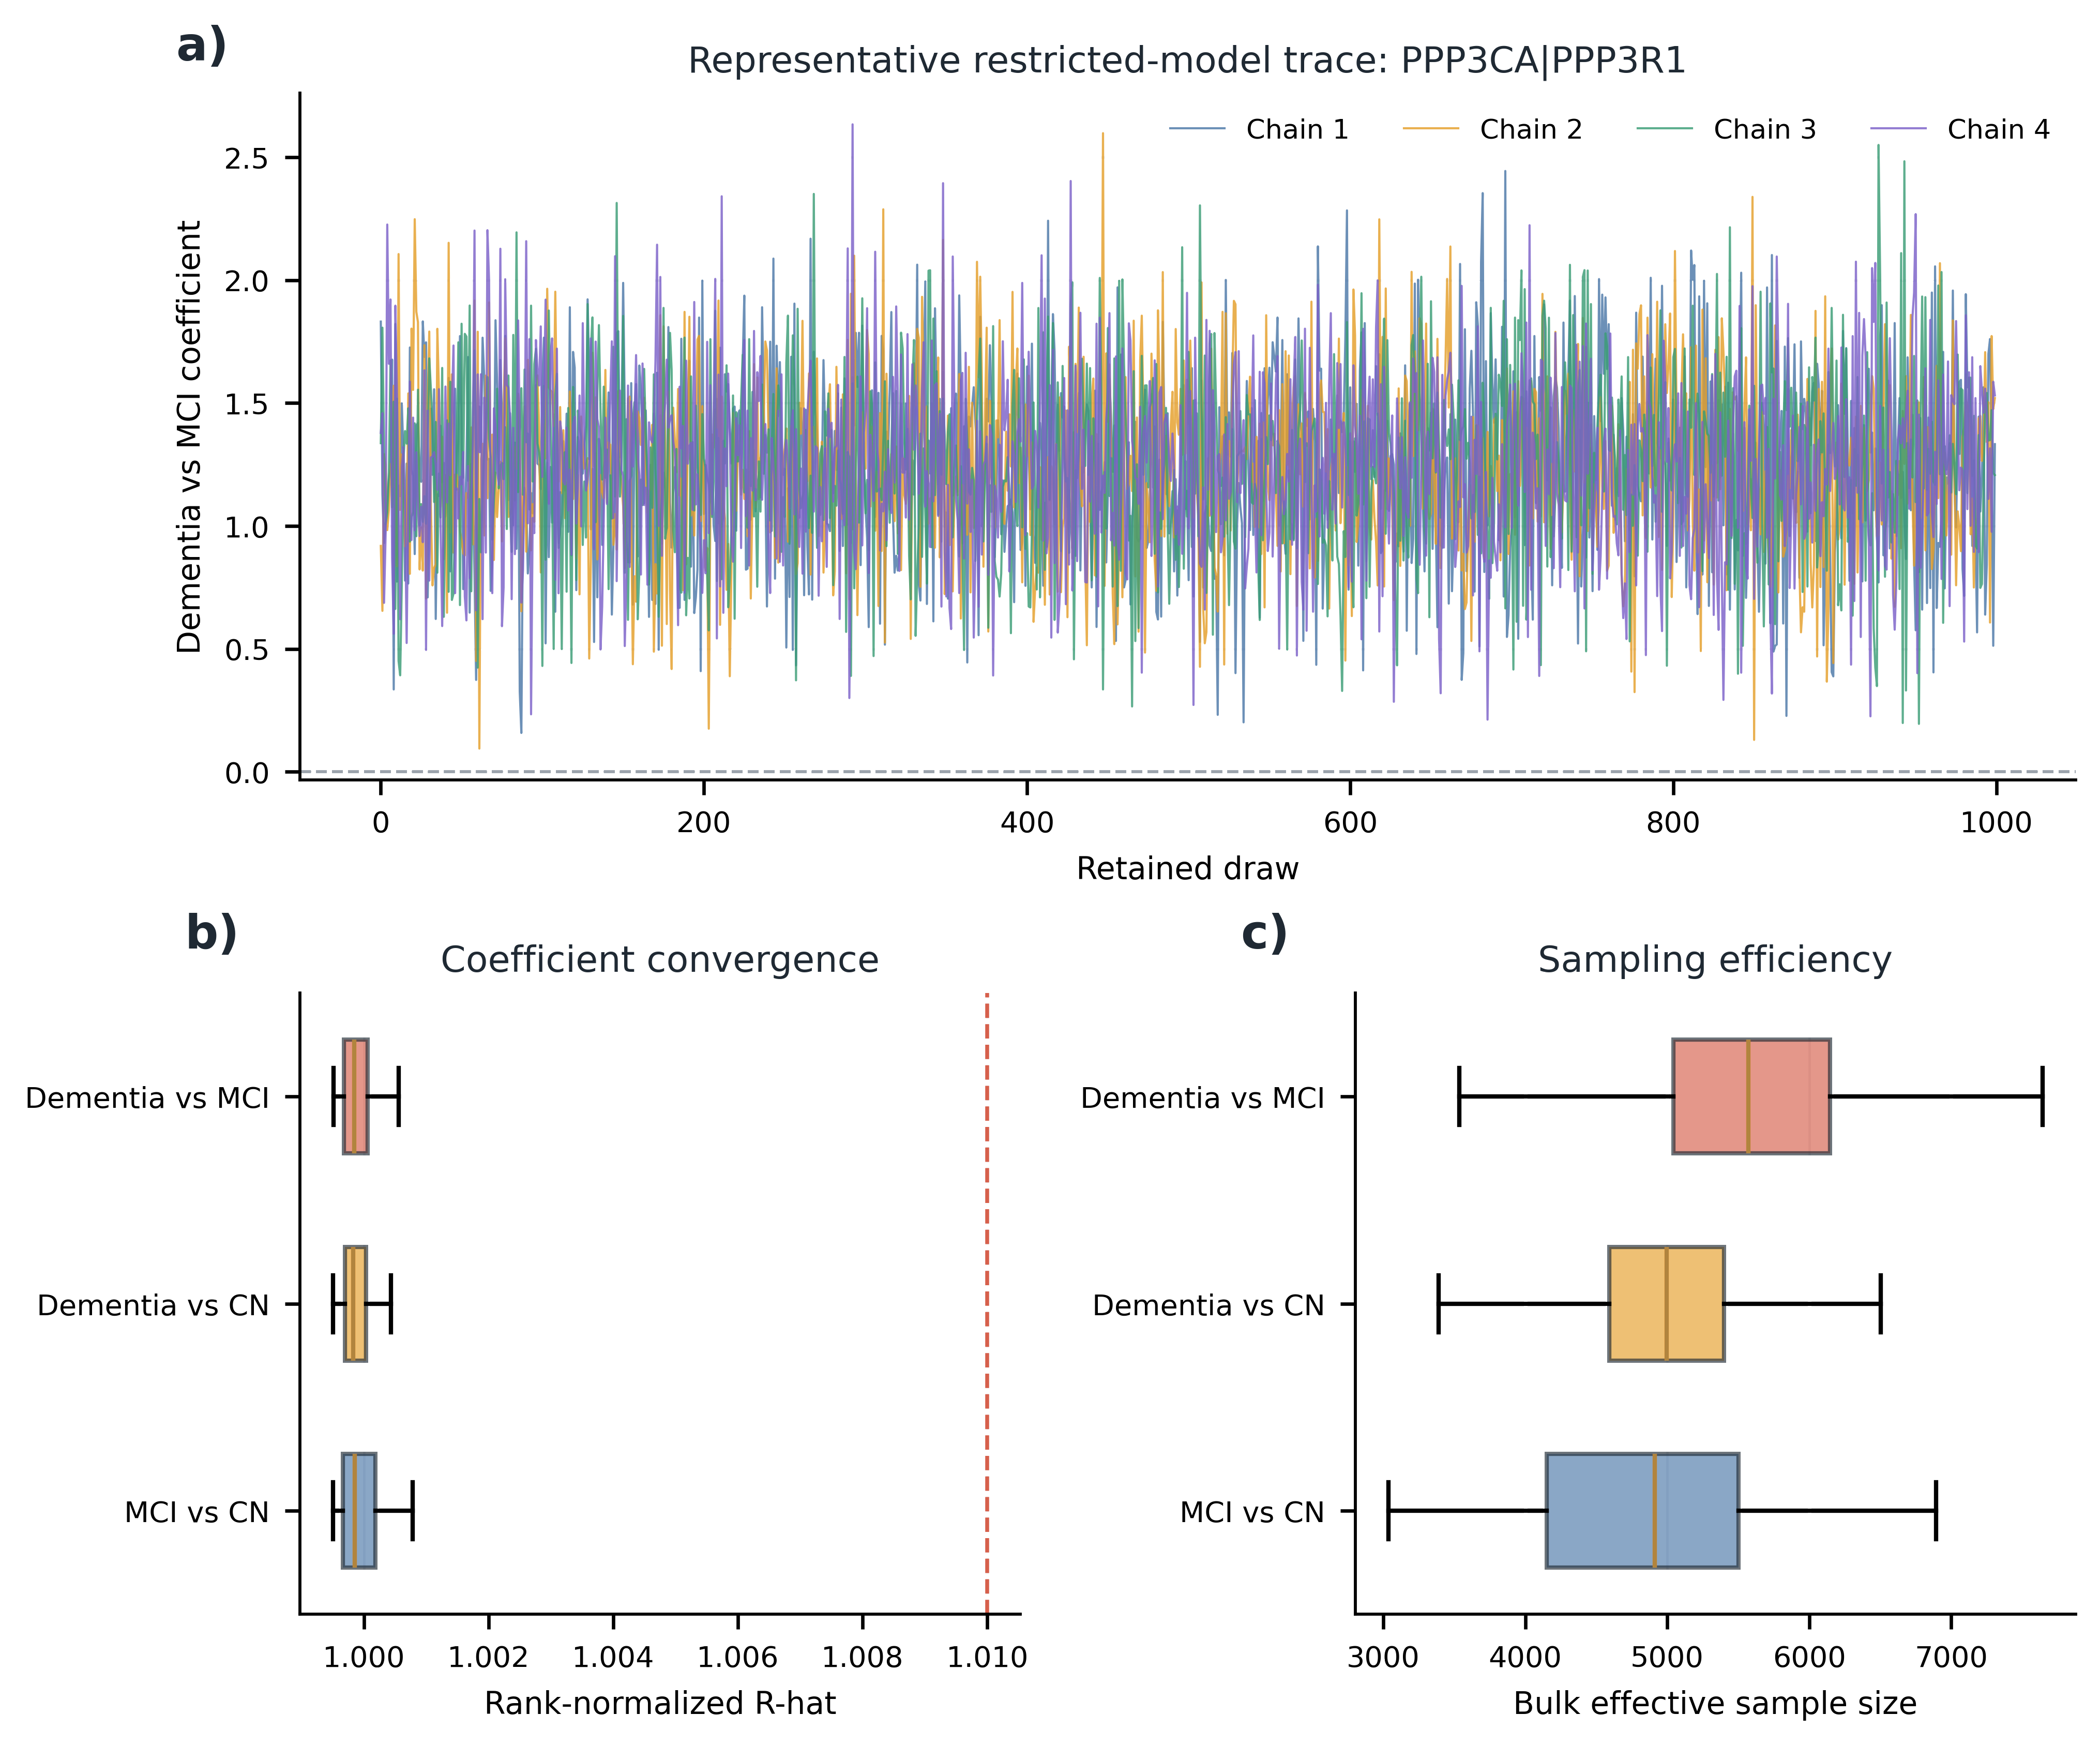
\includegraphics[width=170mm]{figures/figure_s6.png}}
\caption{Restricted Bayesian sampling diagnostics for the development-derived 81-candidate model. a) Representative four-chain trace for the PPP3CA|PPP3R1 dementia-versus-MCI coefficient. b) Rank-normalized R-hat distributions for the three contrasts, with the dashed line at 1.01. c) Bulk effective-sample-size distributions for the three contrasts.}
\label{fig:supp25}
\end{figure}

\begin{figure}[p]
\centering
\makebox[\linewidth][c]{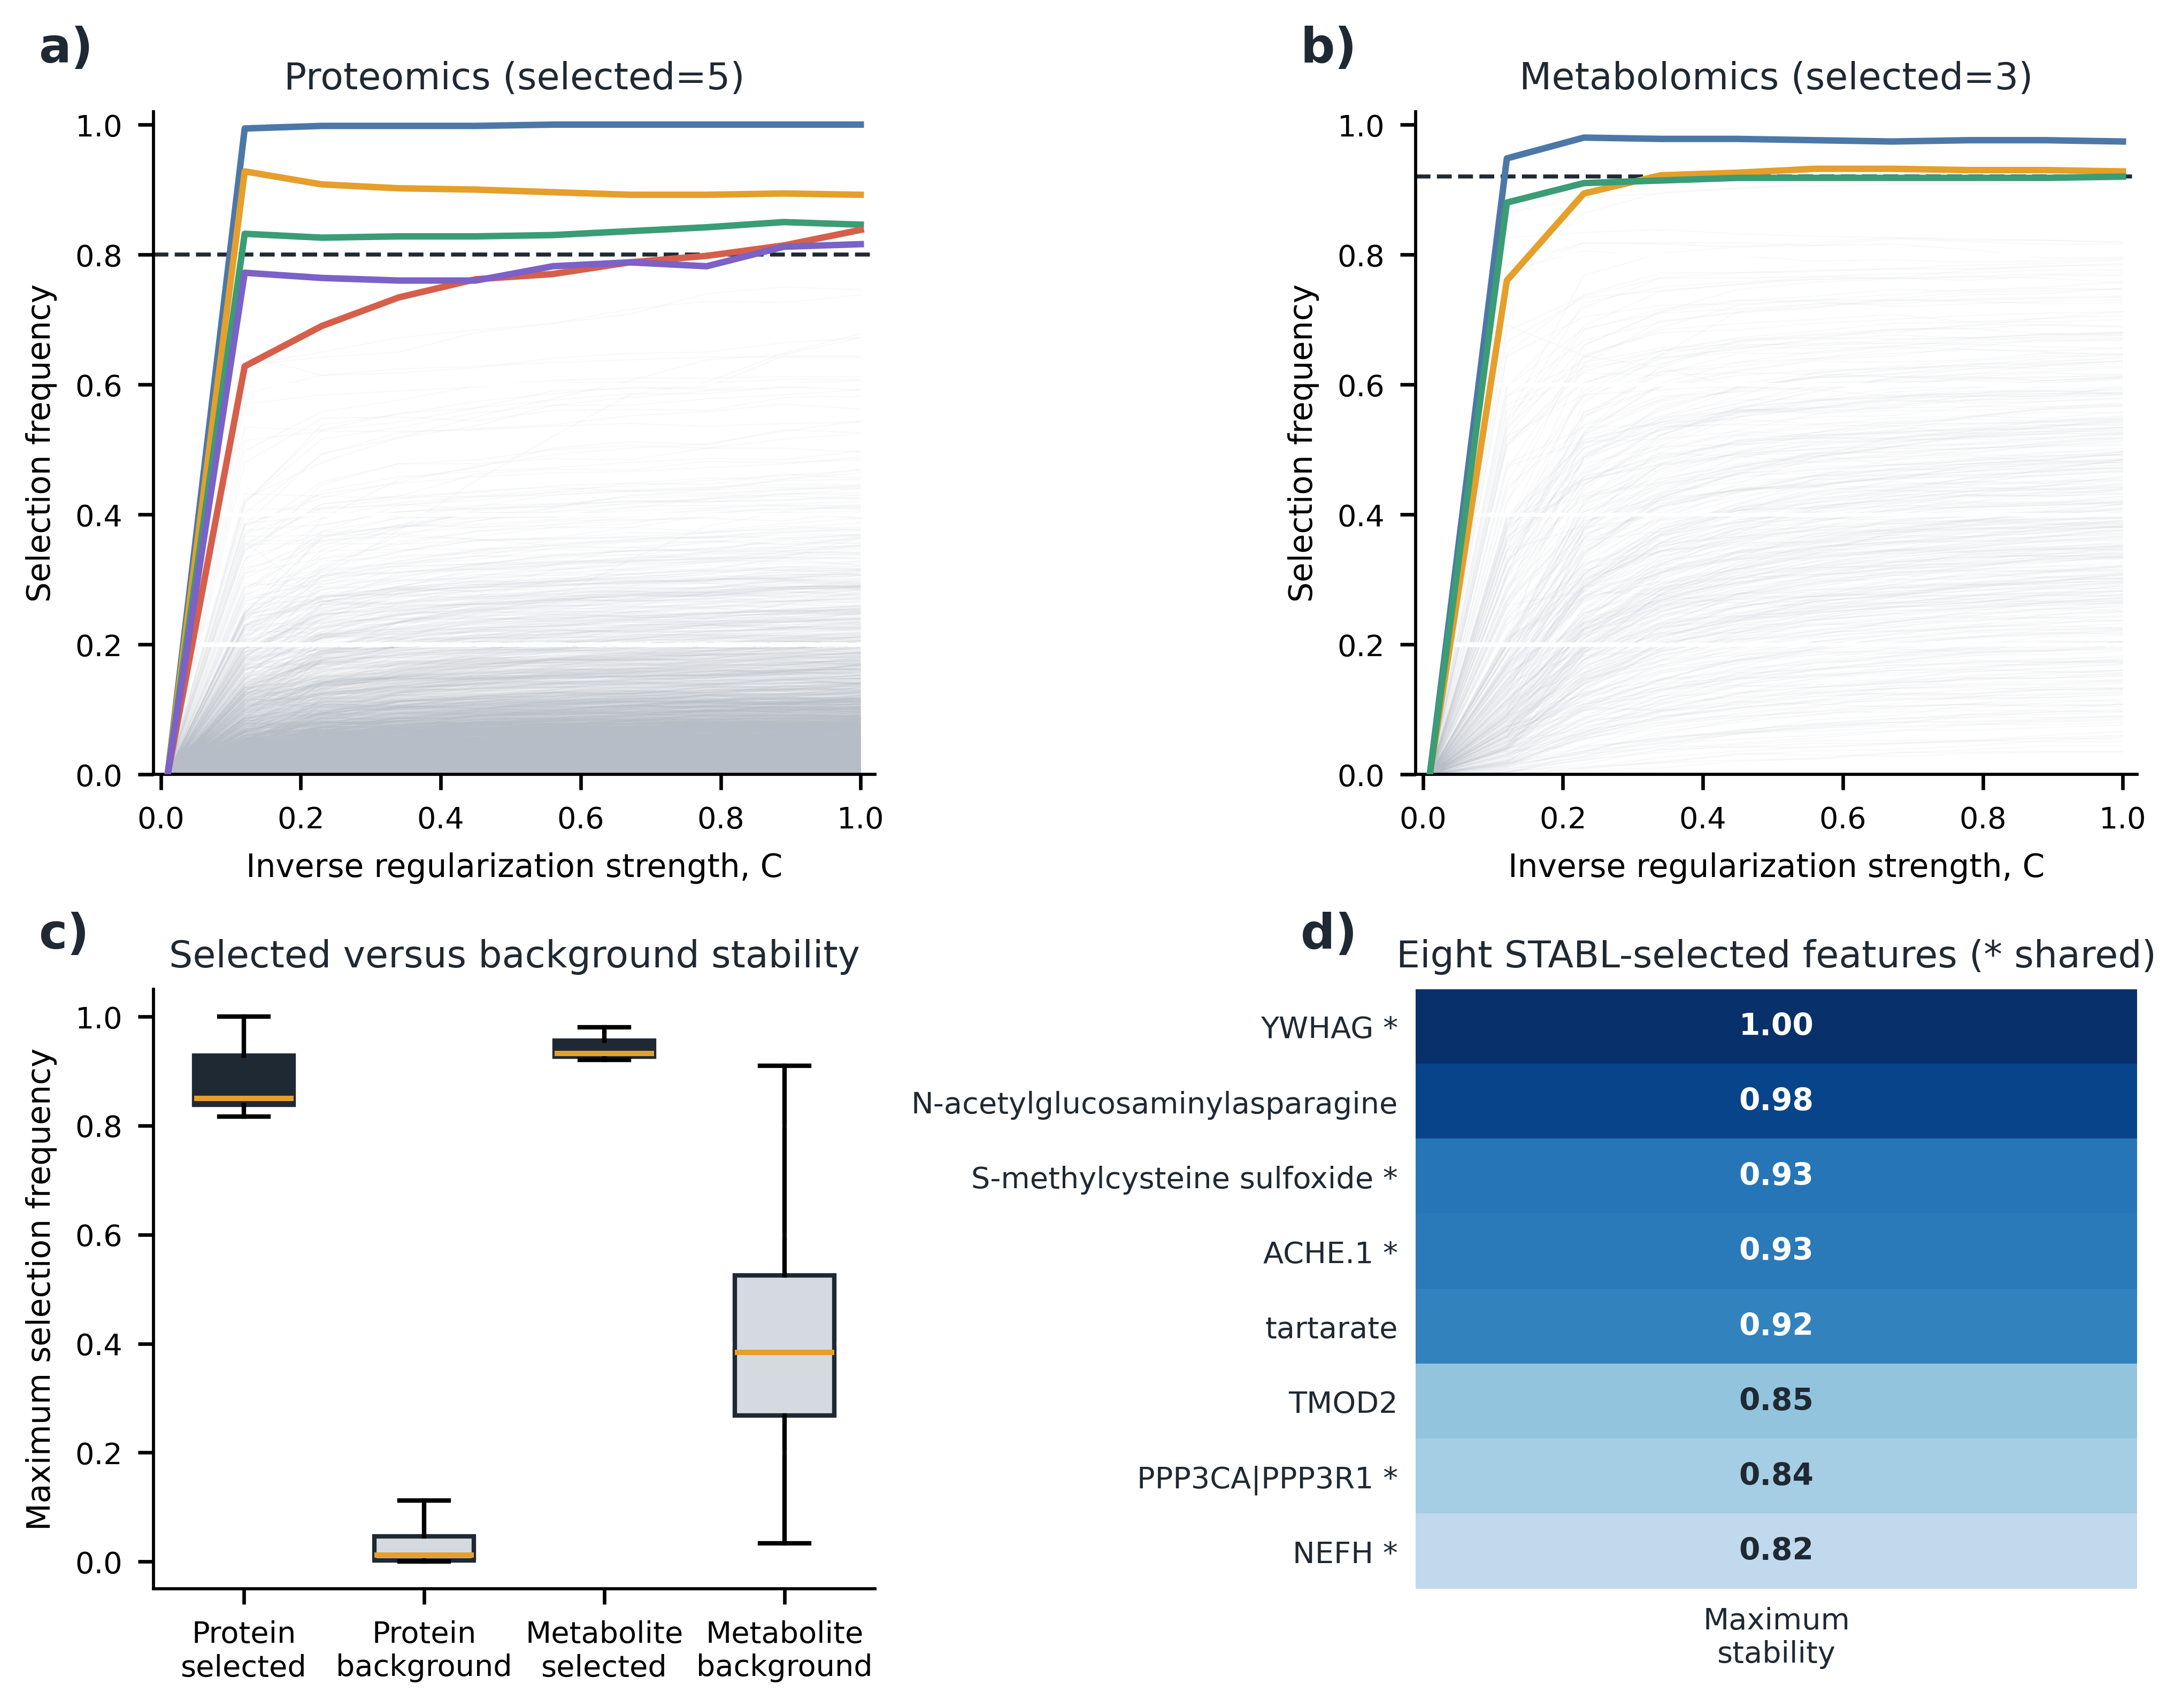
\includegraphics[width=170mm]{figures/figure_s5.png}}
\caption{Training-only STABL analysis. a) Proteomic and b) metabolomic stability paths across inverse regularization strength; colored paths are selected features and dashed lines are selection thresholds. c) Maximum selection-frequency distributions for selected and background features in each omic block. d) Maximum stability for the eight STABL-selected features; asterisks identify features shared with the WrapEvoFS locked-signature union.}
\label{fig:supp26}
\end{figure}

\begin{figure}[p]
\centering
\makebox[\linewidth][c]{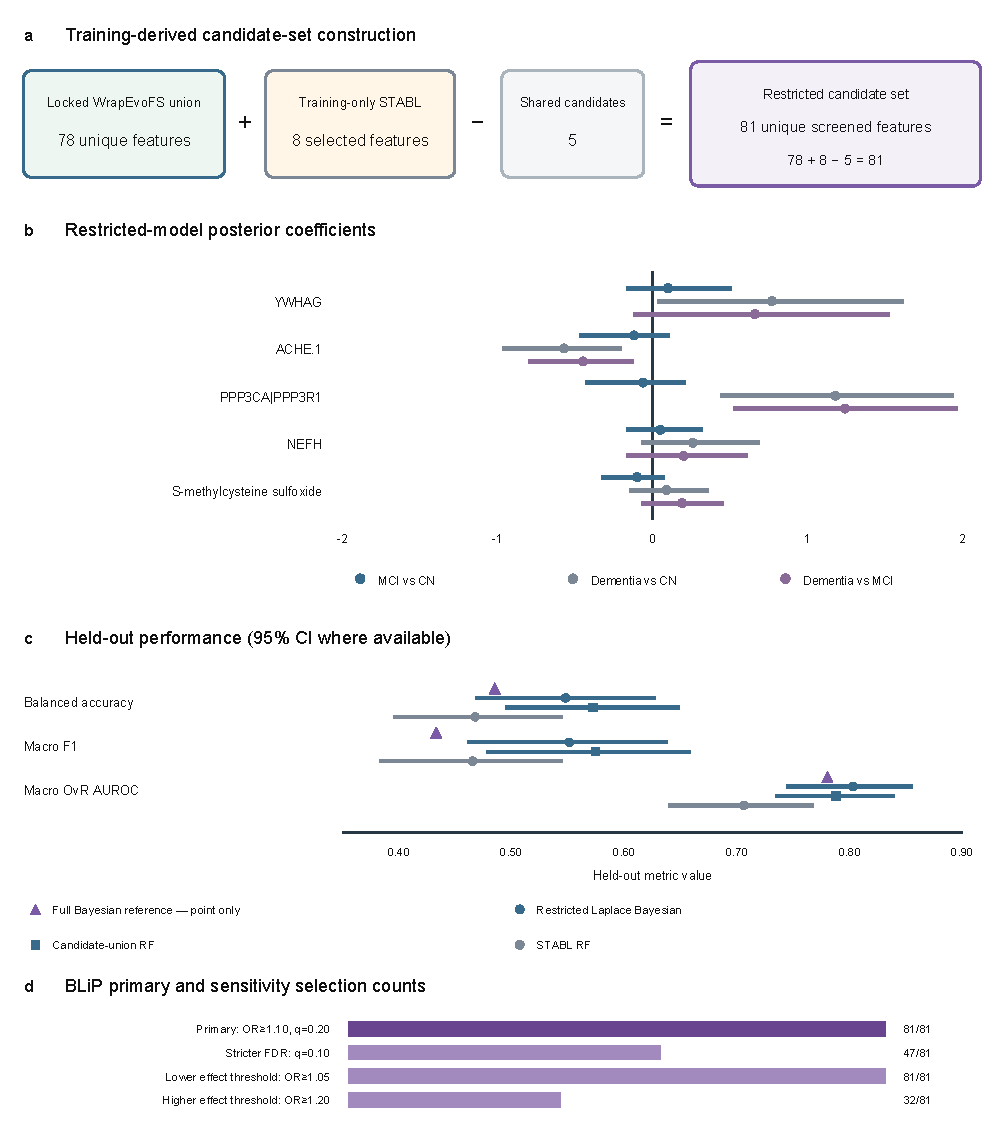
\includegraphics[width=170mm]{figures/supp_polished/supp_s27.pdf}}
\caption{Integrated candidate-restricted Bayesian/STABL/BLiP analysis. a) Training-derived construction of the 81-candidate restricted set from the 78-feature WrapEvoFS union and eight STABL selections with five shared candidates. b) Restricted-model posterior coefficient summaries for the five shared candidates across three dementia contrasts. c) Held-out balanced accuracy, macro F1, and macro one-vs-rest AUROC for the full Bayesian reference (triangles), restricted Laplace Bayesian model (blue circles), candidate-union random forest (blue squares), and STABL random forest (slate circles). d) BLiP selection counts under the primary and sensitivity settings. Primary BLiP retained 81 candidates; stricter-FDR and larger-effect settings retained 47 and 32.}
\label{fig:supp27}
\end{figure}

\begin{figure}[p]
\centering
\makebox[\linewidth][c]{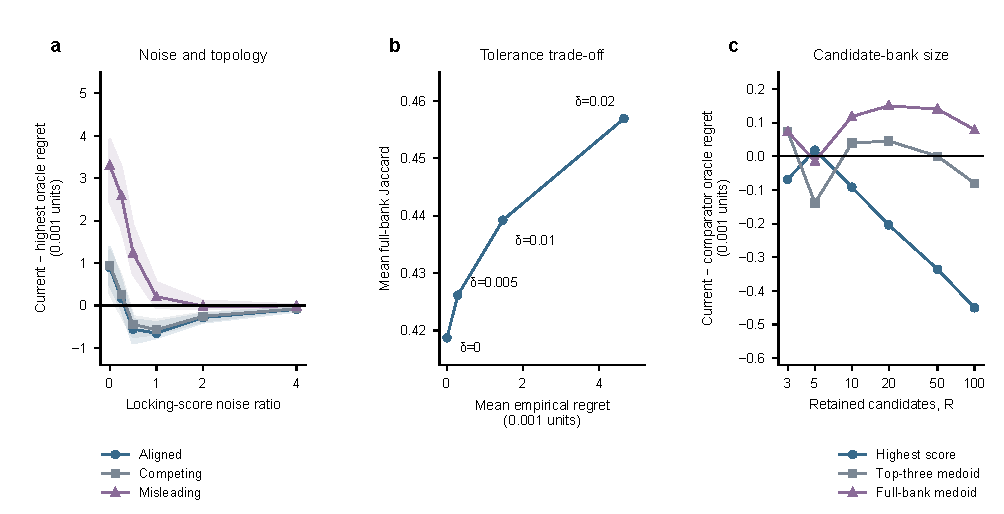
\includegraphics[width=170mm]{v19_work/supplement_polish_20261105/modern/figures/figure_s24.pdf}}
\caption{Controlled synthetic candidate-bank locking simulation. a) Primary equal-scenario mean regret-constrained-medoid-minus-highest-score hidden-oracle regret across locking-score noise ratios and candidate topologies; shaded bands show the interquartile range across nine heterogeneity--proxy combinations. Negative differences favor the regret-constrained medoid. b) Matched 27-scenario tolerance sensitivity showing mean empirical regret against mean full-bank Jaccard; labels identify $\delta$, and increasing tolerance enlarged the eligible pool from 1.00 to 3.69 candidates on average. c) Matched 27-scenario regret-constrained-medoid-minus-comparator hidden-oracle regret across candidate-bank sizes; negative differences favor the regret-constrained medoid. The primary $R=5$, $\delta=0.01$ grid comprised 1,620,000 banks, and the complete sensitivity workload comprised 4,995,000. The regret-constrained medoid had no configured empirical-regret violation. Hidden utility is not AUROC; no GA or classifier was fitted.}
\label{fig:supp28}
\end{figure}

\begin{figure}[p]
\centering
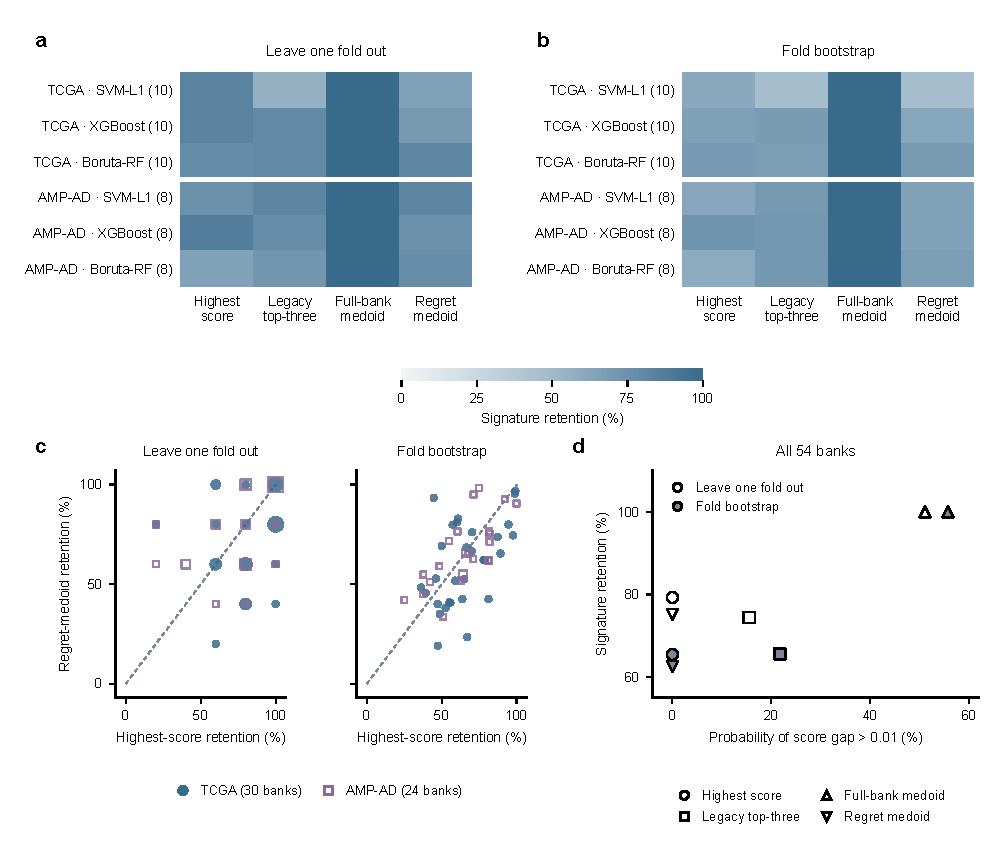
\includegraphics[width=170mm]{v19_work/supplement_polish_20261105/modern/figures/supp_figure_s29_cv_score_sensitivity.pdf}
\caption{Fixed-bank sensitivity to paired development-fold weighting in 54 five-candidate banks (30 TCGA, 24 AMP-AD). Masks and score arrays are fixed; candidates and rules share weights. Retention denotes recovery of each rule's uniform-weight mask. Leave-one-fold-out averages five omissions equally; bootstrap weighting uses multinomial probabilities for 126 count vectors (3,125 ordered resamples).
a,b) Equal-bank mean retention by cohort and branch; parentheses give bank counts.
c) Regret-medoid versus highest-score retention. The diagonal denotes equality; marker area counts exactly coincident banks within each cohort. Both facets reuse the same banks.
d) Equal-bank retention and probability that the perturbed bank-best-minus-selected score exceeds $\delta=0.01$. Open/filled symbols denote leave-one-fold-out/bootstrap weighting; shape denotes rule. Highest-score and regret-constrained exceedance is zero by definition. Unrestricted-medoid retention is 100\% because geometric winners are unchanged. Bootstrap exceedance is 55.76\% for unrestricted and 21.76\% for legacy top-three medoids; regret-medoid and highest-score retention is 62.55\% and 65.44\%, respectively.
Dependent fold scores are reweighted without refitting, held-out access, or participant/bank regeneration. These are descriptive sensitivities, not generalization intervals; no $p$ values are estimated. Mean gaps appear in Supplementary Table~S29.}
\label{fig:supp29}
\end{figure}


\section{Supplementary Tables}

\begin{table}[H]
\centering
\caption{Development-only AMP-AD comparison of the original configuration (zero-truncated objective and top-three Jaccard-medoid locking) with the corrected-objective configuration (untruncated objective and regret-constrained medoid locking at absolute $\delta=0.01$) across 24 combinations of center, branch, and cap. The legacy-zero diagnostic counts generations in which zero truncation would flatten every candidate fitness; it does not count actual sampling fallbacks.}
\label{tab:supp1}
\scriptsize
\setlength{\tabcolsep}{2.6pt}
\renewcommand{\arraystretch}{1.03}
\supplementarytablesection{a. Aggregate target fidelity and flattening diagnostics}
\begin{tabular}{lrrrr}
\toprule
Group & \multicolumn{2}{c}{Absolute target deviation} & \multicolumn{2}{c}{Legacy-zero diagnostic} \\
\cmidrule(lr){2-3}\cmidrule(lr){4-5}
 & Orig. & Upd. & Orig. & Upd. \\
\midrule
Emory & 22 & 15 & 78 & 44 \\
Mayo & 40 & 40 & 132 & 91 \\
Mount Sinai & 44 & 34 & 101 & 65 \\
Rush & 110 & 48 & 362 & 133 \\
\midrule
SVM-L1 & 119 & 62 & 369 & 150 \\
XGBoost & 57 & 62 & 235 & 134 \\
Boruta-RF & 40 & 13 & 69 & 49 \\
\midrule
Overall & 216 & 137 & 673 & 333 \\
\bottomrule
\end{tabular}\par
\vspace{0.75em}
\supplementarytablesection{b. Complete condition-level target and flattening results}
\resizebox{\linewidth}{!}{%
\begin{tabular}{lllrrrrrrrrrr}
\toprule
Center & Branch & Cap & $k^*$ & \multicolumn{2}{c}{Locked $n$} & \multicolumn{2}{c}{$\lvert n-k^*\rvert$} & \multicolumn{2}{c}{Zero run-best, $n/5$} & \multicolumn{2}{c}{Legacy-zero diagnostic} & Upd. regret \\
\cmidrule(lr){5-6}\cmidrule(lr){7-8}\cmidrule(lr){9-10}\cmidrule(lr){11-12}
 & & & & Orig. & Upd. & Orig. & Upd. & Orig. & Upd. & Orig. & Upd. & \\
\midrule
Emory & SVM-L1 & Small & 10 & 12 & 11 & 2 & 1 & 0/5 & 0/5 & 0 & 0 & 0.0000 \\
Emory & SVM-L1 & Reference & 19 & 19 & 19 & 0 & 0 & 0/5 & 0/5 & 0 & 0 & 0.0083 \\
Emory & XGBoost & Small & 9 & 22 & 20 & 13 & 11 & 0/5 & 0/5 & 55 & 29 & 0.0000 \\
Emory & XGBoost & Reference & 17 & 20 & 20 & 3 & 3 & 0/5 & 0/5 & 23 & 15 & 0.0000 \\
Emory & Boruta-RF & Small & 12 & 16 & 12 & 4 & 0 & 0/5 & 0/5 & 0 & 0 & 0.0000 \\
Emory & Boruta-RF & Reference & 25 & 25 & 25 & 0 & 0 & 0/5 & 0/5 & 0 & 0 & 0.0000 \\
\addlinespace[2pt]
Mayo & SVM-L1 & Small & 10 & 26 & 28 & 16 & 18 & 0/5 & 0/5 & 55 & 37 & 0.0000 \\
Mayo & SVM-L1 & Reference & 20 & 23 & 28 & 3 & 8 & 0/5 & 0/5 & 24 & 19 & 0.0000 \\
Mayo & XGBoost & Small & 10 & 22 & 22 & 12 & 12 & 0/5 & 0/5 & 37 & 21 & 0.0000 \\
Mayo & XGBoost & Reference & 20 & 20 & 22 & 0 & 2 & 0/5 & 0/5 & 11 & 9 & 0.0000 \\
Mayo & Boruta-RF & Small & 13 & 22 & 13 & 9 & 0 & 0/5 & 0/5 & 5 & 5 & 0.0000 \\
Mayo & Boruta-RF & Reference & 24 & 24 & 24 & 0 & 0 & 0/5 & 0/5 & 0 & 0 & 0.0020 \\
\addlinespace[2pt]
Mount Sinai & SVM-L1 & Small & 10 & 13 & 12 & 3 & 2 & 0/5 & 0/5 & 0 & 0 & 0.0000 \\
Mount Sinai & SVM-L1 & Reference & 17 & 19 & 17 & 2 & 0 & 0/5 & 0/5 & 0 & 0 & 0.0037 \\
Mount Sinai & XGBoost & Small & 10 & 20 & 24 & 10 & 14 & 0/5 & 0/5 & 31 & 16 & 0.0000 \\
Mount Sinai & XGBoost & Reference & 19 & 22 & 24 & 3 & 5 & 0/5 & 0/5 & 6 & 5 & 0.0000 \\
Mount Sinai & Boruta-RF & Small & 13 & 32 & 24 & 19 & 11 & 0/5 & 0/5 & 39 & 29 & 0.0060 \\
Mount Sinai & Boruta-RF & Reference & 22 & 29 & 24 & 7 & 2 & 0/5 & 0/5 & 25 & 15 & 0.0060 \\
\addlinespace[2pt]
Rush & SVM-L1 & Small & 3 & 84 & 28 & 81 & 25 & 4/5 & 0/5 & 245 & 66 & 0.0000 \\
Rush & SVM-L1 & Reference & 18 & 30 & 26 & 12 & 8 & 0/5 & 0/5 & 45 & 28 & 0.0000 \\
Rush & XGBoost & Small & 7 & 23 & 21 & 16 & 14 & 0/5 & 0/5 & 59 & 30 & 0.0000 \\
Rush & XGBoost & Reference & 20 & 20 & 21 & 0 & 1 & 0/5 & 0/5 & 13 & 9 & 0.0000 \\
Rush & Boruta-RF & Small & 12 & 13 & 12 & 1 & 0 & 0/5 & 0/5 & 0 & 0 & 0.0000 \\
Rush & Boruta-RF & Reference & 23 & 23 & 23 & 0 & 0 & 0/5 & 0/5 & 0 & 0 & 0.0000 \\
\bottomrule
\end{tabular}}
\end{table}

\begin{table}[H]
\ContinuedFloat
\centering
\caption[]{Development-only AMP-AD configuration comparison (continued).}
\scriptsize
\setlength{\tabcolsep}{3.0pt}
\renewcommand{\arraystretch}{1.04}
\supplementarytablesection{c. Fixed development-CV locking score, eligibility, and agreement}
\resizebox{\linewidth}{!}{%
\begin{tabular}{lllrrrrrr}
\toprule
Center & Branch & Cap & \multicolumn{2}{c}{Locking score} & Difference & Eligible $E$ & Upd. regret & Upd. mean Jaccard \\
\cmidrule(lr){4-5}
 & & & Orig. & Upd. & Upd. -- original & & & \\
\midrule
Emory & SVM-L1 & Small & 0.8633 & 0.8501 & -0.0132 & 3 & 0.0000 & 0.1721 \\
Emory & SVM-L1 & Reference & 0.8629 & 0.8609 & -0.0020 & 4 & 0.0083 & 0.3114 \\
Emory & XGBoost & Small & 0.8194 & 0.8235 & 0.0041 & 3 & 0.0000 & 0.1319 \\
Emory & XGBoost & Reference & 0.8207 & 0.8235 & 0.0028 & 3 & 0.0000 & 0.1476 \\
Emory & Boruta-RF & Small & 0.8447 & 0.8488 & 0.0041 & 3 & 0.0000 & 0.1941 \\
Emory & Boruta-RF & Reference & 0.8585 & 0.8629 & 0.0044 & 3 & 0.0000 & 0.3007 \\
\addlinespace[2pt]
Mayo & SVM-L1 & Small & 0.8803 & 0.8803 & -0.0000 & 3 & 0.0000 & 0.1684 \\
Mayo & SVM-L1 & Reference & 0.8800 & 0.8803 & 0.0003 & 3 & 0.0000 & 0.1684 \\
Mayo & XGBoost & Small & 0.8621 & 0.8508 & -0.0113 & 2 & 0.0000 & 0.1795 \\
Mayo & XGBoost & Reference & 0.8269 & 0.8508 & 0.0239 & 2 & 0.0000 & 0.1795 \\
Mayo & Boruta-RF & Small & 0.8705 & 0.8694 & -0.0011 & 2 & 0.0000 & 0.1154 \\
Mayo & Boruta-RF & Reference & 0.8824 & 0.8767 & -0.0058 & 5 & 0.0020 & 0.2407 \\
\addlinespace[2pt]
Mount Sinai & SVM-L1 & Small & 0.8760 & 0.8796 & 0.0036 & 3 & 0.0000 & 0.3125 \\
Mount Sinai & SVM-L1 & Reference & 0.8862 & 0.8920 & 0.0058 & 5 & 0.0037 & 0.2732 \\
Mount Sinai & XGBoost & Small & 0.8613 & 0.8722 & 0.0109 & 2 & 0.0000 & 0.1250 \\
Mount Sinai & XGBoost & Reference & 0.8614 & 0.8722 & 0.0108 & 2 & 0.0000 & 0.1250 \\
Mount Sinai & Boruta-RF & Small & 0.8856 & 0.8804 & -0.0052 & 3 & 0.0060 & 0.1786 \\
Mount Sinai & Boruta-RF & Reference & 0.8821 & 0.8804 & -0.0017 & 3 & 0.0060 & 0.1786 \\
\addlinespace[2pt]
Rush & SVM-L1 & Small & 0.8701 & 0.8602 & -0.0100 & 3 & 0.0000 & 0.1561 \\
Rush & SVM-L1 & Reference & 0.8827 & 0.8735 & -0.0092 & 1 & 0.0000 & NA \\
Rush & XGBoost & Small & 0.8652 & 0.8622 & -0.0030 & 2 & 0.0000 & 0.0833 \\
Rush & XGBoost & Reference & 0.8595 & 0.8631 & 0.0036 & 3 & 0.0000 & 0.1676 \\
Rush & Boruta-RF & Small & 0.8766 & 0.8782 & 0.0017 & 3 & 0.0000 & 0.2982 \\
Rush & Boruta-RF & Reference & 0.8756 & 0.8856 & 0.0100 & 1 & 0.0000 & NA \\
\bottomrule
\end{tabular}}
\vspace{0.55em}
\parbox{0.98\linewidth}{\scriptsize\textit{Note.} Orig., original configuration; Upd., corrected-objective configuration. The original configuration used the zero-truncated objective and legacy top-three medoid. Corrected-objective values were obtained from 120 newly executed full GA runs (five seeds per condition) at the Small and Reference caps using the untruncated objective and regret-constrained medoid; High-cap conditions were not rerun. The legacy-zero column is the zero-truncation diagnostic evaluated along each untruncated search history. Uniform parent-sampling fallbacks were zero. Final locking used fixed development-CV scores, absolute regret tolerance 0.01, strict eligible-only pools, and no fallback expansion. Because both candidate generation and locking differ, between-column differences are configuration-level comparisons rather than isolated causal effects of either component. The two Rush singleton pools have undefined mean Jaccard (NA); all 18 newly completed pools contained two to five candidates. Held-out outcomes were not accessed or evaluated. Mean Jaccard was reduced in canonical mask-hash order. In Mount Sinai/SVM-L1/Reference, runs 3 and 5 had the same exact peer-Jaccard multiset but differed by one IEEE-754 unit in the last place under historical versus canonical reduction order; the authoritative package selected run 5 (17 features; regret 0.0037), whereas the older helper selected run 3 (17 features; regret 0). Both were eligible, and target-count summaries were unchanged.}
\end{table}


\begin{table}[H]
\centering
\caption{Robust development-only summary of the 24-condition AMP-AD original-versus-corrected-objective configuration comparison.}
\label{tab:supp2}
\scriptsize
\setlength{\tabcolsep}{2.8pt}
\renewcommand{\arraystretch}{1.08}
\resizebox{\linewidth}{!}{%
\begin{tabular}{llrrrrrl}
\toprule
Scope & Diagnostic & $n$ & Original & Corrected & Reduction (\%) & Median improvement & Better/unchanged/worse \\
\midrule
All 24 conditions & Absolute target deviation & 24 & 216 & 137 & 79 (36.6\%) & 0.5 & 12/6/6 \\
All 24 conditions & Legacy-zero diagnostic & 24 & 673 & 333 & 340 (50.5\%) & 3.0 & 14/10/0 \\
Excluding Rush/SVM-L1/Small & Absolute target deviation & 23 & 135 & 112 & 23 (17.0\%) & 0.0 & 11/6/6 \\
Excluding Rush/SVM-L1/Small & Legacy-zero diagnostic & 23 & 428 & 267 & 161 (37.6\%) & 2.0 & 13/10/0 \\
\bottomrule
\end{tabular}}
\par\smallskip
\parbox{0.98\linewidth}{\scriptsize\textit{Note.} The legacy-zero diagnostic counts generations whose candidate fitness values would all be zero under legacy truncation; actual uniform parent-sampling fallbacks were zero. The excluded prespecified stress condition is Rush/SVM-L1/Small. Positive improvement denotes a lower corrected-objective value. The stress condition accounts for 56/79 (70.9\%) of the aggregate target-deviation reduction and 179/340 (52.6\%) of the legacy-zero diagnostic reduction; both diagnostics remain lower after exclusion. Held-out outcomes were not accessed.}
\end{table}


\begin{table}[H]
\centering
\caption{Existing-artifact 2 by 2 candidate-bank and locking-rule comparison for matched AMP-AD development conditions.}
\label{tab:supp3}
\scriptsize
\setlength{\tabcolsep}{2.6pt}
\renewcommand{\arraystretch}{1.08}
\resizebox{\linewidth}{!}{%
\begin{tabular}{llrrrrrrr}
\toprule
Candidate bank & Locking rule & $n$ & Total target deviation & Mean selected $n$ & Mean score & Mean regret & Maximum regret & Mask changes \\
\midrule
Original-objective bank & Original top-three & 24 & 216 & 24.12 & 0.86475 & 0.00261 & 0.02111 & 10 \\
Original-objective bank & Regret-constrained & 24 & 227 & 24.58 & 0.86676 & 0.00060 & 0.00729 & 10 \\
Corrected-objective bank & Top-three medoid & 24 & 135 & 20.75 & 0.86329 & 0.00351 & 0.01525 & 8 \\
Corrected-objective bank & Regret-constrained & 24 & 137 & 20.83 & 0.86572 & 0.00108 & 0.00835 & 8 \\
\bottomrule
\end{tabular}}
\par\smallskip
\parbox{0.98\linewidth}{\scriptsize\textit{Note.} No candidate generation or held-out evaluation was rerun. All 24 original-objective banks and all 24 corrected-objective banks were complete after recovery of the 30 Rush run-best feature lists from the authoritative Drive source folder. ``Mask changes'' is the within-bank number of conditions for which the two locking rules selected different masks. The regret-constrained rule improved the configured development-CV score-gap summaries in both bank sets but did not universally improve target fidelity.}
\end{table}


\begin{table}[H]
\centering
\caption{Eligible-pool decision paths and duplicate-mask sensitivity for the 24 corrected-objective AMP-AD development-only conditions at absolute $\delta=0.01$.}
\label{tab:supp4}
\scriptsize
\setlength{\tabcolsep}{4.2pt}
\renewcommand{\arraystretch}{1.08}
\supplementarytablesection{a. Eligible-pool and decision-path audit}
\begin{tabular}{lrr@{\hspace{1.2cm}}lrr}
\toprule
Pool category & Conditions & Percent & Decision stage & Conditions & Percent \\
\midrule
Singleton & 2 & 8.3\% & Singleton direct & 2 & 8.3\% \\
Two candidates & 6 & 25.0\% & Unique Jaccard & 13 & 54.2\% \\
Three or more & 16 & 66.7\% & Higher score & 9 & 37.5\% \\
 & & & Smaller feature count & 0 & 0.0\% \\
 & & & Stable mask hash & 0 & 0.0\% \\
\bottomrule
\end{tabular}

\vspace{0.8em}
\supplementarytablesection{b. Duplicate-retained versus deduplicated sensitivity}
\begin{tabular}{lrrrl}
\toprule
Candidate bank & Audited conditions & Banks with duplicates & Selected-mask changes & Status \\
\midrule
Original-objective & 24 & 0 & 0 & Complete \\
Corrected-objective & 24 & 0 & 0 & Complete after Rush recovery \\
\bottomrule
\end{tabular}
\par\smallskip
\parbox{0.98\linewidth}{\scriptsize\textit{Note.} Exact duplicate masks are retained as multiple voting candidates by the package. No duplicates occurred in the 48 complete banks, so deduplication did not change a selected mask in this empirical sensitivity. The 30 Rush run-best feature lists were recovered from the authoritative Drive source folder; all six current selections matched both the archived summary and the frozen one-time evaluation. Source-run provenance is distinct from input-row order and is used only after scientific feature-set selection when exact duplicates require a provenance representative.}
\end{table}


{
\footnotesize
\renewcommand{\arraystretch}{1.08}
\setlength{\tabcolsep}{2.2pt}
\begin{longtable}{@{}>{\raggedright\arraybackslash}p{0.1326\linewidth}>{\centering\arraybackslash}p{0.1024\linewidth}>{\centering\arraybackslash}p{0.1868\linewidth}>{\centering\arraybackslash}p{0.1868\linewidth}>{\centering\arraybackslash}p{0.2049\linewidth}>{\centering\arraybackslash}p{0.1265\linewidth}@{}}
\caption{AMP-AD development-only representative-run locking sensitivity across 36 completed conditions.}\label{tab:supp5}\\
\toprule
\bfseries Branch & \bfseries Conditions & \bfseries Top-three medoid = highest score & \bfseries Top-three medoid = full-bank medoid & \bfseries Legacy CV regret, median [IQR] & \bfseries Legacy median features \\
\midrule
\endfirsthead
\multicolumn{6}{l}{\footnotesize\itshape \tablename~\thetable\ (continued)}\\
\toprule
\bfseries Branch & \bfseries Conditions & \bfseries Top-three medoid = highest score & \bfseries Top-three medoid = full-bank medoid & \bfseries Legacy CV regret, median [IQR] & \bfseries Legacy median features \\
\midrule
\endhead
\bottomrule
\endfoot
XGBoost & 12 & 8/12 & 4/12 & 0.0000 [0.0000, 0.0025] & 22.0 \\
SVM-L1 & 12 & 5/12 & 5/12 & 0.0016 [0.0000, 0.0037] & 28.0 \\
Boruta-RF & 12 & 8/12 & 5/12 & 0.0000 [0.0000, 0.0021] & 27.0 \\
Overall & 36 & 21/36 & 14/36 & 0.0000 [0.0000, 0.0030] & 24.5 \\
\end{longtable}
}


\begin{table}[H]
\centering
\caption{Fully nested TCGA selector-layer comparator and random-bank sensitivity.}
\label{tab:supp6}
\scriptsize
\setlength{\tabcolsep}{3.4pt}
\renewcommand{\arraystretch}{1.08}
\begin{tabular}{llrrrr}
\toprule
Branch & Selector & Mean features & Macro AUROC & 95\% CI & WrapEvoFS minus selector \tabularnewline
\midrule
SVM-L1 & WrapEvoFS & 14.6 & 0.827 & 0.807--0.845 & Reference \\
 & Elastic Net, native & 73.7 & 0.841 & 0.821--0.861 & $-0.0146$ [$-0.0251$, $-0.0045$] \\
 & Elastic Net, matched & 14.6 & 0.809 & 0.789--0.827 & $+0.0176$ [$+0.0008$, $+0.0341$] \\
 & Stability, native & 58.0 & 0.840 & 0.820--0.859 & $-0.0136$ [$-0.0245$, $-0.0029$] \\
 & Stability, matched & 14.6 & 0.800 & 0.780--0.820 & $+0.0261$ [$+0.0082$, $+0.0434$] \\
\addlinespace
XGBoost & WrapEvoFS & 20.0 & 0.827 & 0.806--0.847 & Reference \\
 & Elastic Net, native & 77.0 & 0.834 & 0.814--0.854 & $-0.0071$ [$-0.0173$, $+0.0037$] \\
 & Elastic Net, matched & 20.0 & 0.829 & 0.809--0.848 & $-0.0017$ [$-0.0146$, $+0.0111$] \\
 & Stability, native & 38.2 & 0.826 & 0.807--0.845 & $+0.0008$ [$-0.0102$, $+0.0119$] \\
 & Stability, matched & 20.0 & 0.829 & 0.809--0.847 & $-0.0015$ [$-0.0136$, $+0.0105$] \\
\addlinespace
Boruta-RF & WrapEvoFS & 18.0 & 0.828 & 0.807--0.847 & Reference \\
 & Elastic Net, native & 60.4 & 0.838 & 0.819--0.857 & $-0.0108$ [$-0.0199$, $-0.0012$] \\
 & Elastic Net, matched & 18.0 & 0.839 & 0.819--0.857 & $-0.0109$ [$-0.0236$, $+0.0024$] \\
 & Stability, native & 30.6 & 0.834 & 0.814--0.852 & $-0.0066$ [$-0.0179$, $+0.0057$] \\
 & Stability, matched & 18.0 & 0.841 & 0.821--0.860 & $-0.0128$ [$-0.0260$, $+0.0012$] \\
\bottomrule
\end{tabular}

\begin{minipage}{0.98\linewidth}\scriptsize\vspace{0.4em}
Macro one-vs-rest AUROC estimates average two repeated five-fold outer-CV OOF estimates. Intervals and paired differences use 2,000 participant-clustered, class-stratified resamples retaining both repeat predictions for each sampled participant. Elastic Net and stability selection were fitted inside each verified post-Direct outer-training universe. Native support is the prespecified primary comparator; matched support uses the same outer-condition cardinality as WrapEvoFS. The five random-bank means were 0.828, 0.817, and 0.832 for SVM-L1, XGBoost, and Boruta-RF, respectively; mean WrapEvoFS-minus-random differences were $-0.0018$, $+0.0102$, and $-0.0043$. Random controls match five-candidate bank size and locking-evaluation budget, not full GA compute. Comparisons are retrospective selector-layer sensitivities and do not establish equivalence or external validity.
\end{minipage}
\end{table}


\begin{table}[H]
\centering
\caption{AMP-AD one-time post-freeze held-out evaluation of the 24 corrected-objective conditions}
\label{tab:supp7}
\scriptsize
\begin{tabularx}{\linewidth}{@{}>{\raggedright\arraybackslash}p{0.12\linewidth}>{\raggedright\arraybackslash}p{0.11\linewidth}>{\centering\arraybackslash}p{0.14\linewidth}>{\centering\arraybackslash}X>{\centering\arraybackslash}X@{}}
\toprule
Branch & Cap & Mean center AUROC & Medoid $-$ RFECV-only & Medoid $-$ top-three medoid \\
\midrule
SVM-L1 & Small & 0.747 & -0.010 [-0.035, +0.014] & -0.031 [-0.055, -0.006] \\
SVM-L1 & Reference & 0.776 & -0.008 [-0.029, +0.012] & +0.012 [-0.009, +0.035] \\
XGBoost & Small & 0.785 & +0.048 [+0.025, +0.070] & +0.018 [-0.003, +0.038] \\
XGBoost & Reference & 0.782 & -0.021 [-0.044, +0.001] & +0.015 [-0.007, +0.037] \\
Boruta-RF & Small & 0.779 & -0.040 [-0.062, -0.019] & -0.012 [-0.033, +0.013] \\
Boruta-RF & Reference & 0.793 & +0.002 [-0.015, +0.019] & +0.015 [-0.003, +0.033] \\
\bottomrule
\end{tabularx}
\begin{minipage}{0.98\linewidth}\scriptsize\vspace{0.3em}
Point estimates in the fourth and fifth columns are pooled four-center macro-AUROC differences with 95\% intervals from 2,000 common resamples stratified by held-out center and true class (seed 42). The 24 development locks and protocol hash were frozen before held-out labels or outcomes were loaded. The evaluation was performed once and did not trigger reselection or retuning. This is post-freeze cross-center evaluation, not prospective clinical or independent external validation.
\end{minipage}
\end{table}


{
\scriptsize
\renewcommand{\arraystretch}{1.08}
\setlength{\tabcolsep}{1.3pt}
\begin{longtable}{@{}>{\raggedright\arraybackslash}p{0.102\linewidth}>{\centering\arraybackslash}p{0.047\linewidth}>{\centering\arraybackslash}p{0.043\linewidth}>{\centering\arraybackslash}p{0.132\linewidth}>{\centering\arraybackslash}p{0.116\linewidth}>{\centering\arraybackslash}p{0.146\linewidth}>{\centering\arraybackslash}p{0.058\linewidth}>{\centering\arraybackslash}p{0.071\linewidth}>{\raggedright\arraybackslash}p{0.176\linewidth}@{}}
\caption{Archived ADNI locking audit and agreement summary. Section a reports the five run-level development-CV candidates under legacy and regret-constrained locking; section b reports the selected-run agreement summary. The larger-is-better locking score is mean balanced accuracy, and absolute regret is measured from the branch maximum. At $\delta=0.01$, each branch had one eligible candidate, marked $\delta$-selected.}\label{tab:supp8}\\
\multicolumn{9}{l}{\footnotesize\bfseries a. Five-run locking audit}\\[0.3em]
\toprule
\bfseries Method & \bfseries GA rank & \bfseries n & \bfseries Balanced accuracy & \bfseries Macro F1 & \bfseries Weighted OvR AUROC & \bfseries Lock rank & \bfseries Abs. regret & \bfseries Status \\
\midrule
\endfirsthead
\multicolumn{9}{l}{\footnotesize\itshape \tablename~\thetable\ (continued)}\\
\toprule
\bfseries Method & \bfseries GA rank & \bfseries n & \bfseries Balanced accuracy & \bfseries Macro F1 & \bfseries Weighted OvR AUROC & \bfseries Lock rank & \bfseries Abs. regret & \bfseries Status \\
\midrule
\endhead
\bottomrule
\endfoot
SVM-L1 & 1 & 29 & 0.563 (0.028) & 0.569 (0.033) & 0.814 (0.011) & 3 & 0.02365 & Top-three medoid \\
SVM-L1 & 2 & 29 & 0.572 (0.055) & 0.579 (0.056) & 0.817 (0.031) & 2 & 0.01401 & Legacy selected \\
SVM-L1 & 3 & 29 & 0.562 (0.053) & 0.568 (0.049) & 0.818 (0.023) & 4 & 0.02463 & --- \\
SVM-L1 & 4 & 29 & 0.586 (0.052) & 0.595 (0.049) & 0.808 (0.040) & 1 & 0 & Top-three medoid; $\delta$-selected \\
SVM-L1 & 5 & 29 & 0.560 (0.029) & 0.565 (0.035) & 0.820 (0.018) & 5 & 0.02596 & --- \\
XGBoost & 1 & 30 & 0.521 (0.032) & 0.520 (0.036) & 0.768 (0.008) & 3 & 0.02168 & Top-three medoid \\
XGBoost & 2 & 30 & 0.542 (0.054) & 0.545 (0.055) & 0.784 (0.034) & 1 & 0 & Legacy and $\delta$-selected \\
XGBoost & 3 & 31 & 0.517 (0.038) & 0.509 (0.043) & 0.767 (0.019) & 4 & 0.02570 & --- \\
XGBoost & 4 & 31 & 0.530 (0.047) & 0.534 (0.052) & 0.772 (0.015) & 2 & 0.01232 & Top-three medoid \\
XGBoost & 5 & 31 & 0.516 (0.031) & 0.513 (0.034) & 0.768 (0.027) & 5 & 0.02618 & --- \\
Boruta-RF & 1 & 27 & 0.574 (0.021) & 0.580 (0.026) & 0.788 (0.020) & 1 & 0 & Top-three medoid; $\delta$-selected \\
Boruta-RF & 2 & 27 & 0.557 (0.020) & 0.563 (0.025) & 0.791 (0.015) & 2 & 0.01713 & Top-three medoid \\
Boruta-RF & 3 & 27 & 0.551 (0.024) & 0.555 (0.025) & 0.783 (0.023) & 3 & 0.02252 & Legacy selected \\
Boruta-RF & 4 & 27 & 0.530 (0.030) & 0.533 (0.029) & 0.780 (0.025) & 5 & 0.04439 & --- \\
Boruta-RF & 5 & 27 & 0.548 (0.016) & 0.554 (0.024) & 0.780 (0.017) & 4 & 0.02553 & --- \\
\end{longtable}
}


\Needspace{9\baselineskip}
\supplementarytablesection{b. Locked-medoid agreement summary}

{
\small
\renewcommand{\arraystretch}{1.08}
\setlength{\tabcolsep}{2.2pt}
\renewcommand{\theHtable}{suppanel.08}% unique anchor for a captionless panel table
\begin{longtable}{@{}>{\raggedright\arraybackslash}p{0.2169\linewidth}>{\centering\arraybackslash}p{0.2169\linewidth}>{\centering\arraybackslash}p{0.5062\linewidth}@{}}
\toprule
\bfseries Method & \bfseries Locked run & \bfseries Mean Jaccard with top three \\
\midrule
\endfirsthead
\toprule
\bfseries Method & \bfseries Locked run & \bfseries Mean Jaccard with top three \\
\midrule
\endhead
\bottomrule
\endfoot
SVM-L1 & 2 & 0.382 \\
XGBoost & 2 & 0.247 \\
Boruta-RF & 3 & 0.385 \\
\end{longtable}
\addtocounter{table}{-1}% captionless panel table must not advance the supplementary-table number
}


{
\scriptsize
\renewcommand{\arraystretch}{1.08}
\setlength{\tabcolsep}{2.2pt}
\begin{longtable}{@{}>{\raggedright\arraybackslash}p{0.1041\linewidth}>{\raggedright\arraybackslash}p{0.1041\linewidth}>{\centering\arraybackslash}p{0.0622\linewidth}>{\centering\arraybackslash}p{0.1634\linewidth}>{\centering\arraybackslash}p{0.1345\linewidth}>{\centering\arraybackslash}p{0.1837\linewidth}>{\centering\arraybackslash}p{0.1880\linewidth}@{}}
\caption{ADNI held-out performance and paired archived top-three medoid-minus-Direct differences. Sections a--d report development-CV summaries, held-out point estimates, class-specific sensitivity, and paired held-out differences, respectively. In this table, ``Locked medoid'' denotes the archived top-three medoid. The development-CV summaries here reproduce the archived final-evaluation fold summary; Supplementary Table~S8 reports the separately recovered run-level locking-evaluator scores used for re-locking. Values may therefore differ for the same archived mask and should not be interchanged.}\label{tab:supp9}\\
\multicolumn{7}{l}{\footnotesize\bfseries a. Development-CV summary}\\[0.3em]
\toprule
\bfseries Method & \bfseries Signature & \bfseries n & \bfseries Balanced accuracy & \bfseries Macro F1 & \bfseries Weighted OvR AUROC & \bfseries Macro OvR AUROC \\
\midrule
\endfirsthead
\multicolumn{7}{l}{\footnotesize\itshape \tablename~\thetable\ (continued)}\\
\toprule
\bfseries Method & \bfseries Signature & \bfseries n & \bfseries Balanced accuracy & \bfseries Macro F1 & \bfseries Weighted OvR AUROC & \bfseries Macro OvR AUROC \\
\midrule
\endhead
\bottomrule
\endfoot
SVM-L1 & Direct & 63 & 0.547 (0.044) & 0.535 (0.058) & 0.825 (0.022) & 0.821 (0.016) \\
SVM-L1 & Locked medoid & 29 & 0.572 (0.055) & 0.579 (0.056) & 0.817 (0.031) & 0.813 (0.025) \\
XGBoost & Direct & 100 & 0.509 (0.041) & 0.502 (0.048) & 0.783 (0.023) & 0.781 (0.023) \\
XGBoost & Locked medoid & 30 & 0.539 (0.038) & 0.539 (0.037) & 0.787 (0.032) & 0.785 (0.024) \\
Boruta-RF & Direct & 48 & 0.549 (0.028) & 0.555 (0.036) & 0.786 (0.016) & 0.784 (0.016) \\
Boruta-RF & Locked medoid & 27 & 0.560 (0.058) & 0.565 (0.063) & 0.779 (0.032) & 0.779 (0.027) \\
\end{longtable}
}


\Needspace{9\baselineskip}
\supplementarytablesection{b. Held-out point estimates}

{
\scriptsize
\renewcommand{\arraystretch}{1.08}
\setlength{\tabcolsep}{2.2pt}
\renewcommand{\theHtable}{suppanel.10}% unique anchor for a captionless panel table
\begin{longtable}{@{}>{\raggedright\arraybackslash}p{0.1041\linewidth}>{\raggedright\arraybackslash}p{0.1041\linewidth}>{\centering\arraybackslash}p{0.1676\linewidth}>{\centering\arraybackslash}p{0.1591\linewidth}>{\centering\arraybackslash}p{0.1475\linewidth}>{\centering\arraybackslash}p{0.1287\linewidth}>{\centering\arraybackslash}p{0.1287\linewidth}@{}}
\toprule
\bfseries Method & \bfseries Signature & \bfseries Balanced accuracy & \bfseries Macro F1 & \bfseries Accuracy & \bfseries Weighted OvR AUROC & \bfseries Macro OvR AUROC \\
\midrule
\endfirsthead
\toprule
\bfseries Method & \bfseries Signature & \bfseries Balanced accuracy & \bfseries Macro F1 & \bfseries Accuracy & \bfseries Weighted OvR AUROC & \bfseries Macro OvR AUROC \\
\midrule
\endhead
\bottomrule
\endfoot
SVM-L1 & Direct & 0.531 [0.460, 0.603] & 0.521 [0.440, 0.606] & 0.617 [0.549, 0.684] & 0.790 [0.734, 0.843] & 0.782 [0.725, 0.833] \\
SVM-L1 & Locked medoid & 0.521 [0.446, 0.604] & 0.517 [0.431, 0.610] & 0.602 [0.526, 0.677] & 0.790 [0.729, 0.841] & 0.784 [0.724, 0.835] \\
XGBoost & Direct & 0.535 [0.469, 0.607] & 0.525 [0.442, 0.610] & 0.624 [0.556, 0.692] & 0.810 [0.754, 0.862] & 0.809 [0.757, 0.858] \\
XGBoost & Locked medoid & 0.564 [0.483, 0.646] & 0.578 [0.482, 0.663] & 0.624 [0.549, 0.699] & 0.775 [0.717, 0.831] & 0.775 [0.720, 0.831] \\
Boruta-RF & Direct & 0.577 [0.494, 0.663] & 0.590 [0.497, 0.675] & 0.624 [0.549, 0.699] & 0.794 [0.739, 0.849] & 0.790 [0.733, 0.845] \\
Boruta-RF & Locked medoid & 0.535 [0.460, 0.610] & 0.540 [0.455, 0.626] & 0.602 [0.526, 0.677] & 0.795 [0.740, 0.849] & 0.788 [0.732, 0.842] \\
\end{longtable}
\addtocounter{table}{-1}% captionless panel table must not advance the supplementary-table number
}


\Needspace{9\baselineskip}
\supplementarytablesection{c. Class-specific sensitivity}

{
\footnotesize
\renewcommand{\arraystretch}{1.08}
\setlength{\tabcolsep}{2.2pt}
\renewcommand{\theHtable}{suppanel.11}% unique anchor for a captionless panel table
\begin{longtable}{@{}>{\raggedright\arraybackslash}p{0.1446\linewidth}>{\raggedright\arraybackslash}p{0.1446\linewidth}>{\centering\arraybackslash}p{0.2169\linewidth}>{\centering\arraybackslash}p{0.2169\linewidth}>{\centering\arraybackslash}p{0.2169\linewidth}@{}}
\toprule
\bfseries Method & \bfseries Signature & \bfseries CN & \bfseries MCI & \bfseries Dementia \\
\midrule
\endfirsthead
\toprule
\bfseries Method & \bfseries Signature & \bfseries CN & \bfseries MCI & \bfseries Dementia \\
\midrule
\endhead
\bottomrule
\endfoot
SVM-L1 & Direct & 0.154 & 0.638 & 0.800 \\
SVM-L1 & Locked medoid & 0.192 & 0.553 & 0.817 \\
XGBoost & Direct & 0.154 & 0.617 & 0.833 \\
XGBoost & Locked medoid & 0.308 & 0.617 & 0.767 \\
Boruta-RF & Direct & 0.385 & 0.596 & 0.750 \\
Boruta-RF & Locked medoid & 0.269 & 0.553 & 0.783 \\
\end{longtable}
\addtocounter{table}{-1}% captionless panel table must not advance the supplementary-table number
}


\Needspace{9\baselineskip}
\supplementarytablesection{d. Paired held-out differences}

{
\footnotesize
\renewcommand{\arraystretch}{1.08}
\setlength{\tabcolsep}{2.2pt}
\renewcommand{\theHtable}{suppanel.12}% unique anchor for a captionless panel table
\begin{longtable}{@{}>{\raggedright\arraybackslash}p{0.1526\linewidth}>{\raggedright\arraybackslash}p{0.2014\linewidth}>{\centering\arraybackslash}p{0.1282\linewidth}>{\centering\arraybackslash}p{0.1281\linewidth}>{\centering\arraybackslash}p{0.1281\linewidth}>{\raggedright\arraybackslash}p{0.2015\linewidth}@{}}
\toprule
\bfseries Method & \bfseries Metric & \bfseries Direct & \bfseries Locked medoid & \bfseries Difference & \bfseries 95\% paired CI \\
\midrule
\endfirsthead
\toprule
\bfseries Method & \bfseries Metric & \bfseries Direct & \bfseries Locked medoid & \bfseries Difference & \bfseries 95\% paired CI \\
\midrule
\endhead
\bottomrule
\endfoot
SVM-L1 & Balanced accuracy & 0.531 & 0.521 & -0.010 & [-0.070, +0.053] \\
SVM-L1 & Macro F1 & 0.521 & 0.517 & -0.004 & [-0.076, +0.071] \\
SVM-L1 & Macro OvR AUROC & 0.782 & 0.784 & +0.001 & [-0.031, +0.035] \\
XGBoost & Balanced accuracy & 0.535 & 0.564 & +0.029 & [-0.047, +0.107] \\
XGBoost & Macro F1 & 0.525 & 0.578 & +0.052 & [-0.044, +0.146] \\
XGBoost & Macro OvR AUROC & 0.809 & 0.775 & -0.034 & [-0.075, +0.004] \\
Boruta-RF & Balanced accuracy & 0.577 & 0.535 & -0.042 & [-0.107, +0.021] \\
Boruta-RF & Macro F1 & 0.590 & 0.540 & -0.050 & [-0.125, +0.022] \\
Boruta-RF & Macro OvR AUROC & 0.790 & 0.788 & -0.002 & [-0.029, +0.026] \\
\end{longtable}
\addtocounter{table}{-1}% captionless panel table must not advance the supplementary-table number
}


{
\footnotesize
\renewcommand{\arraystretch}{1.08}
\setlength{\tabcolsep}{2.2pt}
\begin{longtable}{@{}>{\raggedright\arraybackslash}p{0.1567\linewidth}>{\raggedright\arraybackslash}p{0.1567\linewidth}>{\centering\arraybackslash}p{0.1567\linewidth}>{\centering\arraybackslash}p{0.1567\linewidth}>{\centering\arraybackslash}p{0.1567\linewidth}>{\centering\arraybackslash}p{0.1567\linewidth}@{}}
\caption{AMP-AD pooled performance, paired-interval audit, target tracking, and cross-center recurrence. Sections a--d report pooled point estimates, interval coverage, target fidelity, and locked-signature recurrence, respectively.}\label{tab:supp10}\\
\multicolumn{6}{l}{\footnotesize\bfseries a. Pooled point estimates}\\[0.3em]
\toprule
\bfseries Branch & \bfseries Cap & \bfseries Mean features & \bfseries Macro OvR AUROC [95\% CI] & \bfseries Balanced accuracy [95\% CI] & \bfseries Macro F1 [95\% CI] \\
\midrule
\endfirsthead
\multicolumn{6}{l}{\footnotesize\itshape \tablename~\thetable\ (continued)}\\
\toprule
\bfseries Branch & \bfseries Cap & \bfseries Mean features & \bfseries Macro OvR AUROC [95\% CI] & \bfseries Balanced accuracy [95\% CI] & \bfseries Macro F1 [95\% CI] \\
\midrule
\endhead
\bottomrule
\endfoot
XGBoost & Small & 21.8 & 0.782 [0.755, 0.810] & 0.558 [0.518, 0.600] & 0.559 [0.515, 0.603] \\
XGBoost & Reference & 20.5 & 0.747 [0.717, 0.776] & 0.528 [0.488, 0.566] & 0.521 [0.477, 0.562] \\
XGBoost & High & 33.0 & 0.784 [0.759, 0.811] & 0.542 [0.503, 0.582] & 0.534 [0.493, 0.577] \\
SVM-L1 & Small & 33.8 & 0.769 [0.741, 0.796] & 0.527 [0.486, 0.569] & 0.531 [0.487, 0.574] \\
SVM-L1 & Reference & 22.8 & 0.774 [0.745, 0.802] & 0.556 [0.518, 0.595] & 0.560 [0.519, 0.601] \\
SVM-L1 & High & 36.2 & 0.783 [0.756, 0.809] & 0.520 [0.481, 0.564] & 0.524 [0.480, 0.571] \\
Boruta-RF & Small & 20.8 & 0.763 [0.737, 0.790] & 0.523 [0.486, 0.560] & 0.520 [0.480, 0.559] \\
Boruta-RF & Reference & 25.2 & 0.770 [0.741, 0.797] & 0.555 [0.520, 0.593] & 0.543 [0.505, 0.583] \\
Boruta-RF & High & 47.0 & 0.776 [0.751, 0.801] & 0.526 [0.488, 0.564] & 0.525 [0.485, 0.564] \\
\end{longtable}
}


\Needspace{9\baselineskip}
\supplementarytablesection{b. Paired-interval audit}

{
\small
\renewcommand{\arraystretch}{1.08}
\setlength{\tabcolsep}{2.2pt}
\renewcommand{\theHtable}{suppanel.30}% unique anchor for a captionless panel table
\begin{longtable}{@{}>{\raggedright\arraybackslash}p{0.2350\linewidth}>{\raggedright\arraybackslash}p{0.2350\linewidth}>{\centering\arraybackslash}p{0.2350\linewidth}>{\centering\arraybackslash}p{0.2350\linewidth}@{}}
\toprule
\bfseries Comparison & \bfseries Metric & \bfseries Intervals including zero & \bfseries Conditions \\
\midrule
\endfirsthead
\toprule
\bfseries Comparison & \bfseries Metric & \bfseries Intervals including zero & \bfseries Conditions \\
\midrule
\endhead
\bottomrule
\endfoot
Locked - Direct & macro auroc & 4 & 9 \\
Locked - Direct & balanced accuracy & 8 & 9 \\
Locked - Direct & macro f1 & 8 & 9 \\
Locked - RFECV-only & macro auroc & 4 & 9 \\
Locked - RFECV-only & balanced accuracy & 8 & 9 \\
Locked - RFECV-only & macro f1 & 8 & 9 \\
\end{longtable}
\addtocounter{table}{-1}% captionless panel table must not advance the supplementary-table number
}


\Needspace{9\baselineskip}
\supplementarytablesection{c. Target fidelity and success counts}

{
\small
\renewcommand{\arraystretch}{1.08}
\setlength{\tabcolsep}{2.2pt}
\renewcommand{\theHtable}{suppanel.31}% unique anchor for a captionless panel table
\begin{longtable}{@{}>{\raggedright\arraybackslash}p{0.1747\linewidth}>{\raggedright\arraybackslash}p{0.3917\linewidth}>{\raggedright\arraybackslash}p{0.3736\linewidth}@{}}
\toprule
\bfseries Cap & \bfseries Absolute deviation, features & \bfseries Target attainment, n/12 \\
\midrule
\endfirsthead
\toprule
\bfseries Cap & \bfseries Absolute deviation, features & \bfseries Target attainment, n/12 \\
\midrule
\endhead
\bottomrule
\endfoot
Small & Mean 15.50; median 11.0 [3.75, 16.0] & Exact 0; <=1: 1; <=3: 3 \\
Reference & Mean 2.50; median 1.0 [0, 3.0] & Exact 6; <=1: 6; <=3: 10 \\
High & Mean 0.75; median 0 [0, 1.0] & Exact 8; <=1: 11; <=3: 11 \\
\end{longtable}
\addtocounter{table}{-1}% captionless panel table must not advance the supplementary-table number
}


\Needspace{9\baselineskip}
\supplementarytablesection{d. Locked-signature cross-center recurrence}

{
\footnotesize
\renewcommand{\arraystretch}{1.08}
\setlength{\tabcolsep}{2.2pt}
\renewcommand{\theHtable}{suppanel.32}% unique anchor for a captionless panel table
\begin{longtable}{@{}>{\raggedright\arraybackslash}p{0.1880\linewidth}>{\raggedright\arraybackslash}p{0.1880\linewidth}>{\centering\arraybackslash}p{0.1880\linewidth}>{\centering\arraybackslash}p{0.1880\linewidth}>{\centering\arraybackslash}p{0.1880\linewidth}@{}}
\toprule
\bfseries Branch & \bfseries Cap & \bfseries Mean pairwise Jaccard & \bfseries Minimum & \bfseries Maximum \\
\midrule
\endfirsthead
\toprule
\bfseries Branch & \bfseries Cap & \bfseries Mean pairwise Jaccard & \bfseries Minimum & \bfseries Maximum \\
\midrule
\endhead
\bottomrule
\endfoot
XGBoost & Small & 0.057 & 0.047 & 0.075 \\
XGBoost & Reference & 0.043 & 0.024 & 0.053 \\
XGBoost & High & 0.040 & 0.028 & 0.052 \\
SVM-L1 & Small & 0.042 & 0.000 & 0.087 \\
SVM-L1 & Reference & 0.077 & 0.039 & 0.188 \\
SVM-L1 & High & 0.080 & 0.013 & 0.143 \\
Boruta-RF & Small & 0.086 & 0.023 & 0.143 \\
Boruta-RF & Reference & 0.084 & 0.040 & 0.143 \\
Boruta-RF & High & 0.157 & 0.094 & 0.218 \\
\end{longtable}
\addtocounter{table}{-1}% captionless panel table must not advance the supplementary-table number
}


{
\footnotesize
\renewcommand{\arraystretch}{1.08}
\setlength{\tabcolsep}{2.2pt}
\begin{longtable}{@{}>{\raggedright\arraybackslash}p{0.1446\linewidth}>{\raggedright\arraybackslash}p{0.1567\linewidth}>{\centering\arraybackslash}p{0.1506\linewidth}>{\centering\arraybackslash}p{0.1265\linewidth}>{\centering\arraybackslash}p{0.1687\linewidth}>{\centering\arraybackslash}p{0.1928\linewidth}@{}}
\caption{AMP-AD ordinal outcome sensitivity using existing pooled leave-one-center-out predictions. Sections a and b report locked-medoid point estimates and paired locked-medoid-minus-Direct differences, respectively.}\label{tab:supp11}\\
\multicolumn{6}{l}{\footnotesize\bfseries a. Locked-medoid point estimates}\\[0.3em]
\toprule
\bfseries Branch & \bfseries Cap & \bfseries Mean features & \bfseries QWK & \bfseries Ordinal MAE & \bfseries Severe-error rate \\
\midrule
\endfirsthead
\multicolumn{6}{l}{\footnotesize\itshape \tablename~\thetable\ (continued)}\\
\toprule
\bfseries Branch & \bfseries Cap & \bfseries Mean features & \bfseries QWK & \bfseries Ordinal MAE & \bfseries Severe-error rate \\
\midrule
\endhead
\bottomrule
\endfoot
XGBoost & Small & 21.8 & 0.598 & 0.412 & 0.042 \\
XGBoost & Reference & 20.5 & 0.521 & 0.463 & 0.072 \\
XGBoost & High & 33.0 & 0.585 & 0.429 & 0.049 \\
SVM-L1 & Small & 33.8 & 0.537 & 0.452 & 0.042 \\
SVM-L1 & Reference & 22.8 & 0.555 & 0.427 & 0.055 \\
SVM-L1 & High & 36.2 & 0.499 & 0.459 & 0.057 \\
Boruta-RF & Small & 20.8 & 0.559 & 0.448 & 0.049 \\
Boruta-RF & Reference & 25.2 & 0.598 & 0.423 & 0.049 \\
Boruta-RF & High & 47.0 & 0.573 & 0.444 & 0.042 \\
\end{longtable}
}


\Needspace{9\baselineskip}
\supplementarytablesection{b. Paired locked-medoid-minus-Direct differences}

{
\footnotesize
\renewcommand{\arraystretch}{1.08}
\setlength{\tabcolsep}{2.2pt}
\renewcommand{\theHtable}{suppanel.34}% unique anchor for a captionless panel table
\begin{longtable}{@{}>{\raggedright\arraybackslash}p{0.1265\linewidth}>{\raggedright\arraybackslash}p{0.1446\linewidth}>{\centering\arraybackslash}p{0.2169\linewidth}>{\centering\arraybackslash}p{0.2260\linewidth}>{\centering\arraybackslash}p{0.2260\linewidth}@{}}
\toprule
\bfseries Branch & \bfseries Cap & \bfseries Delta QWK [95\% CI] & \bfseries Delta ordinal MAE [95\% CI] & \bfseries Delta severe-error rate [95\% CI] \\
\midrule
\endfirsthead
\toprule
\bfseries Branch & \bfseries Cap & \bfseries Delta QWK [95\% CI] & \bfseries Delta ordinal MAE [95\% CI] & \bfseries Delta severe-error rate [95\% CI] \\
\midrule
\endhead
\bottomrule
\endfoot
XGBoost & Small & +0.094 [+0.035, +0.153] & -0.017 [-0.059, +0.027] & -0.027 [-0.044, -0.009] \\
XGBoost & Reference & +0.017 [-0.048, +0.081] & +0.034 [-0.009, +0.080] & +0.004 [-0.013, +0.023] \\
XGBoost & High & +0.081 [+0.025, +0.140] & +0.000 [-0.042, +0.040] & -0.019 [-0.036, -0.002] \\
SVM-L1 & Small & +0.070 [+0.014, +0.129] & -0.038 [-0.082, +0.006] & -0.038 [-0.055, -0.021] \\
SVM-L1 & Reference & +0.088 [+0.033, +0.144] & -0.063 [-0.102, -0.021] & -0.025 [-0.042, -0.009] \\
SVM-L1 & High & +0.032 [-0.030, +0.093] & -0.030 [-0.072, +0.009] & -0.023 [-0.040, -0.006] \\
Boruta-RF & Small & -0.018 [-0.060, +0.020] & +0.013 [-0.019, +0.047] & +0.002 [-0.009, +0.013] \\
Boruta-RF & Reference & +0.020 [-0.016, +0.055] & -0.011 [-0.042, +0.021] & +0.002 [-0.008, +0.011] \\
Boruta-RF & High & -0.005 [-0.050, +0.040] & +0.009 [-0.023, +0.044] & -0.006 [-0.021, +0.008] \\
\end{longtable}
\addtocounter{table}{-1}% captionless panel table must not advance the supplementary-table number
}


{\footnotesize\noindent\textit{Note.} Low, Moderate, and High were encoded 0, 1, and 2. Severe errors are direct Low-to-High or High-to-Low classifications. Intervals use 2,000 common resamples stratified by held-out center and true class (seed 42). Negative MAE and severe-error differences favor the locked signature.\par}

{
\scriptsize
\renewcommand{\arraystretch}{1.08}
\setlength{\tabcolsep}{2.2pt}
\begin{longtable}{@{}>{\raggedright\arraybackslash}p{0.1265\linewidth}>{\centering\arraybackslash}p{0.0603\linewidth}>{\centering\arraybackslash}p{0.1567\linewidth}>{\centering\arraybackslash}p{0.1627\linewidth}>{\centering\arraybackslash}p{0.1265\linewidth}>{\centering\arraybackslash}p{0.1476\linewidth}>{\centering\arraybackslash}p{0.1597\linewidth}@{}}
\caption{AMP-AD cohort characteristics and ordered bScore mapping.}\label{tab:supp12}\\
\toprule
\bfseries Center & \bfseries n & \bfseries Low / Moderate / High & \bfseries Age at death, median [IQR] & \bfseries Female, n (\%) & \bfseries APOE4 positive / known & \bfseries PMI, median [IQR] \\
\midrule
\endfirsthead
\multicolumn{7}{l}{\footnotesize\itshape \tablename~\thetable\ (continued)}\\
\toprule
\bfseries Center & \bfseries n & \bfseries Low / Moderate / High & \bfseries Age at death, median [IQR] & \bfseries Female, n (\%) & \bfseries APOE4 positive / known & \bfseries PMI, median [IQR] \\
\midrule
\endhead
\bottomrule
\endfoot
Overall & 527 & 111 / 156 / 260 & 81.7 [73.0, 88.0] & 307 (58.3\%) & 225/516 (43.6\%) & 8.0 [5.1, 14.5]; n=428 \\
Emory & 80 & 19 / 5 / 56 & 75.0 [61.0, 82.0] & 47 (58.8\%) & 47/78 (60.3\%) & 7.0 [4.5, 15.1]; n=80 \\
Mayo & 217 & 51 / 53 / 113 & 79.0 [71.0, 85.0] & 114 (52.5\%) & 91/217 (41.9\%) & 11.0 [5.0, 20.8]; n=118 \\
Mount Sinai & 52 & 9 / 15 / 28 & 82.0 [76.8, 90.0] & 28 (53.8\%) & 20/52 (38.5\%) & 6.9 [4.1, 10.0]; n=52 \\
Rush & 178 & 32 / 83 / 63 & 85.2 [78.7, 90.0] & 118 (66.3\%) & 67/169 (39.6\%) & 7.6 [5.8, 12.5]; n=178 \\
\end{longtable}
}


\Needspace{9\baselineskip}
\supplementarytablesection{b. Source-to-analysis bScore mapping}

{
\small
\renewcommand{\arraystretch}{1.08}
\setlength{\tabcolsep}{2.2pt}
\renewcommand{\theHtable}{suppanel.36}% unique anchor for a captionless panel table
\begin{longtable}{@{}>{\raggedright\arraybackslash}p{0.5122\linewidth}>{\raggedright\arraybackslash}p{0.2651\linewidth}>{\centering\arraybackslash}p{0.1627\linewidth}@{}}
\toprule
\bfseries Source bScore label & \bfseries Analysis class & \bfseries Ordinal code \\
\midrule
\endfirsthead
\toprule
\bfseries Source bScore label & \bfseries Analysis class & \bfseries Ordinal code \\
\midrule
\endhead
\bottomrule
\endfoot
None (Stage 0) & Low & 0 \\
Low (Stage I-II) & Low & 0 \\
Moderate (Stage III-IV) & Moderate & 1 \\
High (Stage V-VI) & High & 2 \\
\end{longtable}
\addtocounter{table}{-1}% captionless panel table must not advance the supplementary-table number
}


{\footnotesize\noindent\textit{Note.} The local raw-to-analysis bundle contained 529 common frontal-proteomic/metabolomic profiles; two participants with unavailable or unrecognized bScore were excluded. Age values recorded as 90+ were represented by the lower-bound value 90 for median and IQR summaries. APOE4 percentages use participants with known yes/no status; PMI availability is reported in the final column.\par}

{
\scriptsize
\renewcommand{\arraystretch}{1.08}
\setlength{\tabcolsep}{1.3pt}
\begin{longtable}{@{}>{\raggedright\arraybackslash}p{0.1106\linewidth}>{\raggedright\arraybackslash}p{0.1162\linewidth}>{\raggedright\arraybackslash}p{0.1714\linewidth}>{\centering\arraybackslash}p{0.0609\linewidth}>{\centering\arraybackslash}p{0.0553\linewidth}>{\centering\arraybackslash}p{0.1162\linewidth}>{\centering\arraybackslash}p{0.0940\linewidth}>{\centering\arraybackslash}p{0.1106\linewidth}>{\raggedright\arraybackslash}p{0.1048\linewidth}@{}}
\caption{CGGA archived-candidate sensitivity comparing the original top-three locking pool with alternative retrospective rules.}\label{tab:supp13}\\
\toprule
\bfseries Method & \bfseries Condition & \bfseries Rule & \bfseries Run & \bfseries n & \bfseries Dev-CV AUROC & \bfseries CV regret & \bfseries Mean Jaccard & \bfseries Matches recorded \\
\midrule
\endfirsthead
\multicolumn{9}{l}{\footnotesize\itshape \tablename~\thetable\ (continued)}\\
\toprule
\bfseries Method & \bfseries Condition & \bfseries Rule & \bfseries Run & \bfseries n & \bfseries Dev-CV AUROC & \bfseries CV regret & \bfseries Mean Jaccard & \bfseries Matches recorded \\
\midrule
\endhead
\bottomrule
\endfoot
SVM-L1 & No guidance & Highest dev-CV & 1 & 16 & 0.880 & 0.000 & - & No \\
SVM-L1 & No guidance & Top-three medoid & 4 & 23 & 0.876 & 0.004 & 0.588 & Yes \\
SVM-L1 & No guidance & All-five medoid & 4 & 23 & 0.876 & 0.004 & 0.522 & Yes \\
SVM-L1 & Guided & Highest dev-CV & 1 & 15 & 0.873 & 0.000 & - & No \\
SVM-L1 & Guided & Top-three medoid & 4 & 16 & 0.870 & 0.003 & 0.476 & Yes \\
SVM-L1 & Guided & All-five medoid & 3 & 15 & 0.859 & 0.015 & 0.465 & No \\
XGBoost & No guidance & Highest dev-CV & 3 & 35 & 0.868 & 0.000 & - & Yes \\
XGBoost & No guidance & Top-three medoid & 3 & 35 & 0.868 & 0.000 & 0.372 & Yes \\
XGBoost & No guidance & All-five medoid & 5 & 39 & 0.843 & 0.025 & 0.412 & No \\
XGBoost & Guided & Highest dev-CV & 2 & 20 & 0.849 & 0.000 & - & No \\
XGBoost & Guided & Top-three medoid & 1 & 19 & 0.846 & 0.003 & 0.295 & Yes \\
XGBoost & Guided & All-five medoid & 1 & 19 & 0.846 & 0.003 & 0.239 & Yes \\
Boruta-RF & No guidance & Highest dev-CV & 4 & 10 & 0.817 & 0.000 & - & No \\
Boruta-RF & No guidance & Top-three medoid & 2 & 14 & 0.803 & 0.015 & 0.535 & Yes \\
Boruta-RF & No guidance & All-five medoid & 2 & 14 & 0.803 & 0.015 & 0.541 & Yes \\
Boruta-RF & Guided & Highest dev-CV & 5 & 9 & 0.815 & 0.000 & - & Yes \\
Boruta-RF & Guided & Top-three medoid & 5 & 9 & 0.815 & 0.000 & 0.442 & Yes \\
Boruta-RF & Guided & All-five medoid & 2 & 9 & 0.799 & 0.016 & 0.452 & No \\
\end{longtable}
{\footnotesize\noindent\textit{Note.} All displayed rules used only the five saved development-run candidates. The highest-development-CV rule ignores overlap; the unrestricted full-bank medoid expands the pool from the three candidates used by the top-three medoid to all five. For every row, CV regret is the highest saved development-CV macro-AUROC minus the score of the candidate selected by that displayed rule. Detailed condition-level records are supplied as a machine-readable companion.\par}
}


{
\scriptsize
\renewcommand{\arraystretch}{1.08}
\setlength{\tabcolsep}{1.3pt}
\begin{longtable}{@{}>{\raggedright\arraybackslash}p{0.1480\linewidth}>{\raggedright\arraybackslash}p{0.1480\linewidth}>{\centering\arraybackslash}p{0.1480\linewidth}>{\centering\arraybackslash}p{0.1287\linewidth}>{\centering\arraybackslash}p{0.0838\linewidth}>{\centering\arraybackslash}p{0.0902\linewidth}>{\centering\arraybackslash}p{0.0901\linewidth}>{\centering\arraybackslash}p{0.1031\linewidth}@{}}
\caption{CGGA condition-level feature recurrence across five saved GA runs. Feature-level records are machine-readable companions.}\label{tab:supp13}\\
\toprule
\bfseries Method & \bfseries Condition & \bfseries Candidate universe & \bfseries Mean n/run & \bfseries 5/5 & \bfseries >=4/5 & \bfseries >=3/5 & \bfseries Any run \\
\midrule
\endfirsthead
\multicolumn{8}{l}{\footnotesize\itshape \tablename~\thetable\ (continued)}\\
\toprule
\bfseries Method & \bfseries Condition & \bfseries Candidate universe & \bfseries Mean n/run & \bfseries 5/5 & \bfseries >=4/5 & \bfseries >=3/5 & \bfseries Any run \\
\midrule
\endhead
\bottomrule
\endfoot
SVM-L1 & No guidance & 35 & 19.0 & 5 & 13 & 18 & 33 \\
SVM-L1 & Guided & 35 & 15.2 & 4 & 7 & 16 & 27 \\
XGBoost & No guidance & 70 & 35.6 & 3 & 15 & 40 & 65 \\
XGBoost & Guided & 70 & 20.0 & 1 & 4 & 13 & 53 \\
Boruta-RF & No guidance & 26 & 11.6 & 3 & 7 & 12 & 19 \\
Boruta-RF & Guided & 26 & 9.0 & 3 & 5 & 6 & 20 \\
\end{longtable}
}


{
\footnotesize
\renewcommand{\arraystretch}{1.08}
\setlength{\tabcolsep}{2.2pt}
\begin{longtable}{@{}>{\raggedright\arraybackslash}p{0.1567\linewidth}>{\raggedright\arraybackslash}p{0.1567\linewidth}>{\centering\arraybackslash}p{0.1567\linewidth}>{\centering\arraybackslash}p{0.1567\linewidth}>{\centering\arraybackslash}p{0.1567\linewidth}>{\centering\arraybackslash}p{0.1567\linewidth}@{}}
\caption{CGGA component-ablation summary with held-out intervals under the fixed random forest. In this table, ``Locked medoid'' denotes the archived legacy top-three medoid. The archived evaluation protocol is retained; Supplementary Table~S17 provides the coherent same-estimator comparison.}\label{tab:supp15}\\
\toprule
\bfseries Method & \bfseries Variant & \bfseries Features, n & \bfseries AUROC [95\% CI] & \bfseries AUPRC [95\% CI] & \bfseries Balanced accuracy [95\% CI] \\
\midrule
\endfirsthead
\multicolumn{6}{l}{\footnotesize\itshape \tablename~\thetable\ (continued)}\\
\toprule
\bfseries Method & \bfseries Variant & \bfseries Features, n & \bfseries AUROC [95\% CI] & \bfseries AUPRC [95\% CI] & \bfseries Balanced accuracy [95\% CI] \\
\midrule
\endhead
\bottomrule
\endfoot
SVM-L1 & Direct & 35 & 0.635 [0.515, 0.741] & 0.639 [0.540, 0.762] & 0.629 [0.531, 0.726] \\
SVM-L1 & RFECV-only & 15 & 0.633 [0.509, 0.741] & 0.615 [0.526, 0.751] & 0.596 [0.498, 0.694] \\
SVM-L1 & Single GA run & 15 & 0.664 [0.546, 0.769] & 0.663 [0.560, 0.788] & 0.629 [0.530, 0.726] \\
SVM-L1 & Best-development-CV run & 15 & 0.664 [0.546, 0.769] & 0.663 [0.560, 0.788] & 0.629 [0.530, 0.726] \\
SVM-L1 & Locked medoid & 16 & 0.652 [0.535, 0.761] & 0.640 [0.548, 0.775] & 0.608 [0.509, 0.705] \\
SVM-L1 & No target-size guidance & 23 & 0.623 [0.497, 0.733] & 0.598 [0.512, 0.737] & 0.618 [0.520, 0.715] \\
XGBoost & Direct & 70 & 0.684 [0.565, 0.785] & 0.675 [0.573, 0.797] & 0.652 [0.552, 0.749] \\
XGBoost & RFECV-only & 20 & 0.675 [0.553, 0.773] & 0.685 [0.582, 0.789] & 0.620 [0.512, 0.716] \\
XGBoost & Single GA run & 19 & 0.702 [0.587, 0.803] & 0.689 [0.592, 0.820] & 0.672 [0.574, 0.761] \\
XGBoost & Best-development-CV run & 20 & 0.716 [0.599, 0.811] & 0.732 [0.630, 0.854] & 0.684 [0.586, 0.772] \\
XGBoost & Locked medoid & 19 & 0.702 [0.587, 0.803] & 0.689 [0.592, 0.820] & 0.672 [0.574, 0.761] \\
XGBoost & No target-size guidance & 35 & 0.645 [0.525, 0.753] & 0.632 [0.539, 0.766] & 0.673 [0.575, 0.762] \\
Boruta-RF & Direct & 26 & 0.658 [0.538, 0.765] & 0.646 [0.554, 0.780] & 0.629 [0.531, 0.727] \\
Boruta-RF & RFECV-only & 9 & 0.682 [0.565, 0.785] & 0.653 [0.558, 0.781] & 0.651 [0.552, 0.748] \\
Boruta-RF & Single GA run & 9 & 0.685 [0.574, 0.790] & 0.732 [0.635, 0.825] & 0.673 [0.576, 0.762] \\
Boruta-RF & Best-development-CV run & 9 & 0.695 [0.582, 0.793] & 0.689 [0.593, 0.810] & 0.652 [0.554, 0.739] \\
Boruta-RF & Locked medoid & 9 & 0.695 [0.582, 0.793] & 0.689 [0.593, 0.810] & 0.652 [0.554, 0.739] \\
Boruta-RF & No target-size guidance & 14 & 0.666 [0.550, 0.773] & 0.661 [0.565, 0.779] & 0.663 [0.565, 0.751] \\
\end{longtable}
}


\Needspace{10\baselineskip}
{
\footnotesize
\renewcommand{\arraystretch}{1.08}
\setlength{\tabcolsep}{2.2pt}
\begin{longtable}{@{}>{\raggedright\arraybackslash}p{0.1864\linewidth}>{\raggedright\arraybackslash}p{0.2187\linewidth}>{\centering\arraybackslash}p{0.0730\linewidth}>{\centering\arraybackslash}p{0.1215\linewidth}>{\centering\arraybackslash}p{0.1215\linewidth}>{\centering\arraybackslash}p{0.2188\linewidth}@{}}
\caption{Exploratory CGGA same-size random-subset and Elastic Net comparator results. Sections a--c report matched-size point estimates, random-subset tail summaries, and paired locked-medoid-minus-Elastic Net differences, respectively. In this table, ``Locked medoid'' denotes the archived top-three medoid. The archived evaluation protocol is retained; Supplementary Table~S17 provides the coherent same-estimator comparison.}\label{tab:supp16}\\
\multicolumn{6}{l}{\footnotesize\bfseries a. Matched-size point estimates}\\[0.3em]
\toprule
\bfseries Method & \bfseries Comparator & \bfseries n & \bfseries AUROC & \bfseries AUPRC & \bfseries Balanced accuracy \\
\midrule
\endfirsthead
\multicolumn{6}{l}{\footnotesize\itshape \tablename~\thetable\ (continued)}\\
\toprule
\bfseries Method & \bfseries Comparator & \bfseries n & \bfseries AUROC & \bfseries AUPRC & \bfseries Balanced accuracy \\
\midrule
\endhead
\bottomrule
\endfoot
SVM-L1 & Locked medoid & 16 & 0.656 & 0.642 & 0.597 \\
SVM-L1 & Elastic Net & 16 & 0.635 & 0.599 & 0.661 \\
XGBoost & Locked medoid & 19 & 0.689 & 0.669 & 0.695 \\
XGBoost & Elastic Net & 19 & 0.640 & 0.623 & 0.617 \\
Boruta-RF & Locked medoid & 9 & 0.694 & 0.700 & 0.652 \\
Boruta-RF & Elastic Net & 9 & 0.612 & 0.608 & 0.607 \\
\end{longtable}
}


\Needspace{9\baselineskip}
\supplementarytablesection{b. Random-subset tail summaries}

{
\scriptsize
\renewcommand{\arraystretch}{1.08}
\setlength{\tabcolsep}{2.2pt}
\renewcommand{\theHtable}{suppanel.25}% unique anchor for a captionless panel table
\begin{longtable}{@{}>{\raggedright\arraybackslash}p{0.1353\linewidth}>{\raggedright\arraybackslash}p{0.1638\linewidth}>{\raggedright\arraybackslash}p{0.1567\linewidth}>{\centering\arraybackslash}p{0.1068\linewidth}>{\centering\arraybackslash}p{0.1139\linewidth}>{\centering\arraybackslash}p{0.1210\linewidth}>{\centering\arraybackslash}p{0.1426\linewidth}@{}}
\toprule
\bfseries Method & \bfseries Metric & \bfseries Comparator & \bfseries Observed & \bfseries Null mean & \bfseries Percentile & \bfseries p (one-sided) \\
\midrule
\endfirsthead
\toprule
\bfseries Method & \bfseries Metric & \bfseries Comparator & \bfseries Observed & \bfseries Null mean & \bfseries Percentile & \bfseries p (one-sided) \\
\midrule
\endhead
\bottomrule
\endfoot
SVM-L1 & AUROC & Locked medoid & 0.656 & 0.615 & 84.3 & 0.162 \\
SVM-L1 & AUROC & Elastic Net & 0.635 & 0.615 & 67.5 & 0.326 \\
SVM-L1 & AUPRC & Locked medoid & 0.642 & 0.619 & 71.5 & 0.286 \\
SVM-L1 & AUPRC & Elastic Net & 0.599 & 0.619 & 32.8 & 0.672 \\
SVM-L1 & Balanced accuracy & Locked medoid & 0.597 & 0.585 & 67.0 & 0.348 \\
SVM-L1 & Balanced accuracy & Elastic Net & 0.661 & 0.585 & 98.2 & 0.019 \\
XGBoost & AUROC & Locked medoid & 0.689 & 0.620 & 94.3 & 0.058 \\
XGBoost & AUROC & Elastic Net & 0.640 & 0.620 & 64.7 & 0.357 \\
XGBoost & AUPRC & Locked medoid & 0.669 & 0.624 & 83.8 & 0.163 \\
XGBoost & AUPRC & Elastic Net & 0.623 & 0.624 & 48.9 & 0.511 \\
XGBoost & Balanced accuracy & Locked medoid & 0.695 & 0.592 & 99.3 & 0.008 \\
XGBoost & Balanced accuracy & Elastic Net & 0.617 & 0.592 & 68.3 & 0.319 \\
Boruta-RF & AUROC & Locked medoid & 0.694 & 0.637 & 95.0 & 0.052 \\
Boruta-RF & AUROC & Elastic Net & 0.612 & 0.637 & 23.4 & 0.767 \\
Boruta-RF & AUPRC & Locked medoid & 0.700 & 0.631 & 93.5 & 0.066 \\
Boruta-RF & AUPRC & Elastic Net & 0.608 & 0.631 & 31.5 & 0.685 \\
Boruta-RF & Balanced accuracy & Locked medoid & 0.652 & 0.619 & 87.0 & 0.135 \\
Boruta-RF & Balanced accuracy & Elastic Net & 0.607 & 0.619 & 33.0 & 0.684 \\
\end{longtable}
\addtocounter{table}{-1}% captionless panel table must not advance the supplementary-table number
}


\Needspace{9\baselineskip}
\supplementarytablesection{c. Paired locked-medoid-minus-Elastic Net differences}

{
\footnotesize
\renewcommand{\arraystretch}{1.08}
\setlength{\tabcolsep}{2.2pt}
\renewcommand{\theHtable}{suppanel.26}% unique anchor for a captionless panel table
\begin{longtable}{@{}>{\raggedright\arraybackslash}p{0.1787\linewidth}>{\raggedright\arraybackslash}p{0.2175\linewidth}>{\centering\arraybackslash}p{0.1399\linewidth}>{\raggedright\arraybackslash}p{0.2719\linewidth}>{\centering\arraybackslash}p{0.1321\linewidth}@{}}
\toprule
\bfseries Method & \bfseries Metric & \bfseries Difference & \bfseries 95\% bootstrap CI & \bfseries Resamples \\
\midrule
\endfirsthead
\toprule
\bfseries Method & \bfseries Metric & \bfseries Difference & \bfseries 95\% bootstrap CI & \bfseries Resamples \\
\midrule
\endhead
\bottomrule
\endfoot
SVM-L1 & AUROC & +0.021 & [-0.083, +0.131] & 2,000 \\
SVM-L1 & AUPRC & +0.043 & [-0.060, +0.149] & 2,000 \\
SVM-L1 & Balanced accuracy & -0.063 & [-0.173, +0.047] & 2,000 \\
XGBoost & AUROC & +0.049 & [-0.059, +0.170] & 2,000 \\
XGBoost & AUPRC & +0.045 & [-0.062, +0.171] & 2,000 \\
XGBoost & Balanced accuracy & +0.078 & [-0.031, +0.196] & 2,000 \\
Boruta-RF & AUROC & +0.082 & [-0.030, +0.200] & 2,000 \\
Boruta-RF & AUPRC & +0.093 & [-0.035, +0.200] & 2,000 \\
Boruta-RF & Balanced accuracy & +0.046 & [-0.075, +0.165] & 2,000 \\
\end{longtable}
\addtocounter{table}{-1}% captionless panel table must not advance the supplementary-table number
}


\begin{table}[H]
\centering
\caption{CGGA coherent same-split, same-estimator benchmark}
\label{tab:supp17}
\scriptsize
\begin{tabular}{llrccc}
\toprule
Branch & Development-derived signature & Features & Held-out AUROC (95\% CI) & AUPRC & Balanced accuracy \\
\midrule
SVM-L1 & RFECV-only & 15 & 0.633 [0.509, 0.741] & 0.615 & 0.596 \\
SVM-L1 & Elastic Net & 16 & 0.644 [0.523, 0.754] & 0.611 & 0.649 \\
SVM-L1 & Highest CV & 15 & 0.664 [0.546, 0.769] & 0.663 & 0.629 \\
SVM-L1 & Top-three medoid & 16 & 0.652 [0.535, 0.761] & 0.640 & 0.608 \\
SVM-L1 & Full-bank medoid & 15 & 0.672 [0.551, 0.776] & 0.672 & 0.652 \\
SVM-L1 & Regret-constrained medoid & 16 & 0.652 [0.535, 0.761] & 0.640 & 0.608 \\
XGBoost & RFECV-only & 20 & 0.680 [0.561, 0.779] & 0.677 & 0.663 \\
XGBoost & Elastic Net & 19 & 0.636 [0.513, 0.746] & 0.622 & 0.639 \\
XGBoost & Highest CV & 20 & 0.699 [0.581, 0.799] & 0.719 & 0.684 \\
XGBoost & Top-three medoid & 19 & 0.700 [0.582, 0.805] & 0.685 & 0.695 \\
XGBoost & Full-bank medoid & 19 & 0.700 [0.582, 0.805] & 0.685 & 0.695 \\
XGBoost & Regret-constrained medoid & 21 & 0.645 [0.527, 0.750] & 0.686 & 0.554 \\
Boruta-RF & RFECV-only & 9 & 0.686 [0.571, 0.788] & 0.669 & 0.629 \\
Boruta-RF & Elastic Net & 9 & 0.606 [0.487, 0.716] & 0.598 & 0.596 \\
Boruta-RF & Highest CV & 9 & 0.694 [0.582, 0.792] & 0.700 & 0.652 \\
Boruta-RF & Top-three medoid & 9 & 0.694 [0.582, 0.792] & 0.700 & 0.652 \\
Boruta-RF & Full-bank medoid & 9 & 0.704 [0.594, 0.804] & 0.674 & 0.695 \\
Boruta-RF & Regret-constrained medoid & 9 & 0.694 [0.582, 0.792] & 0.700 & 0.652 \\
\bottomrule
\end{tabular}
\begin{minipage}{0.98\linewidth}\scriptsize\vspace{0.3em}
All signatures use the same fixed 214/92 split and the same 500-tree random forest (maximum depth 12, minimum leaf size 2, balanced class weighting, random state 42). Feature selection was completed within development data before held-out evaluation. Intervals use 2,000 class-stratified resamples (seed 42). Elastic Net signatures were size matched within branch. No comparison establishes predictive superiority; paired contrasts are shown in Supplementary Fig.~S18c and supplied machine-readable outputs.
\end{minipage}
\end{table}


\begin{table}[H]
\centering
\caption{CGGA saved nested-bank re-locking using the regret-constrained medoid}
\label{tab:supp18}
\scriptsize
\begin{tabular}{rrrrrrrr}
\toprule
Fold & Legacy run & Selected run & Features & Eligible & Regret & Legacy AUROC & Selected AUROC \\
\midrule
1 & 0 & 3 & 15 & 2 & 0.0000 & 0.762 & 0.703 \\
2 & 2 & 4 & 16 & 2 & 0.0000 & 0.615 & 0.621 \\
3 & 1 & 2 & 15 & 1 & 0.0000 & 0.784 & 0.779 \\
4 & 4 & 0 & 15 & 1 & 0.0000 & 0.745 & 0.675 \\
5 & 0 & 2 & 15 & 2 & 0.0000 & 0.600 & 0.573 \\
\bottomrule
\end{tabular}
\begin{minipage}{0.98\linewidth}\scriptsize\vspace{0.3em}
This post hoc internal sensitivity reuses five archived candidate banks from a reduced search budget (20 individuals, 12 generations, five runs) and does not rerun the GA or access the original 92-participant held-out cohort. The regret-constrained medoid changed the selected run in all five outer folds. OOF AUROC was 0.692 for the top-three medoid and 0.667 for the regret-constrained medoid; this adverse result is retained because the regret guarantee concerns the configured development score gap.
\end{minipage}
\end{table}


\begin{table}[H]
\centering
\caption{Private MGMT radiomics internal demonstration under the updated WrapEvoFS configuration.}
\label{tab:supp18}
\scriptsize
\setlength{\tabcolsep}{3.0pt}
\renewcommand{\arraystretch}{1.08}
\textit{A. Development-only feature counts and strict locking audit}\par\smallskip
\begin{tabular}{llrrrrrrrr}
\toprule
Feature space & Branch & Direct & RFECV $k^*$ & Five-run range & Locked & Compression & $|E_{0.01}|$ & Regret \\
\midrule
Full 1,781 & SVM-L1 & 214 & 8 & 50--62 & 50 & 76.6\% & 1 & 0.0000 \\
Full 1,781 & XGBoost & 100 & 16 & 17--24 & 24 & 76.0\% & 1 & 0.0000 \\
Full 1,781 & Boruta-RF & 10 & 10 & 9--10 & 9 & 10.0\% & 2 & 0.0000 \\
Filtered 1,346 & SVM-L1 & 201 & 3 & 46--52 & 50 & 75.1\% & 1 & 0.0000 \\
Filtered 1,346 & XGBoost & 100 & 6 & 17--22 & 19 & 81.0\% & 1 & 0.0000 \\
Filtered 1,346 & Boruta-RF & 6 & 6 & 4--6 & 5 & 16.7\% & 1 & 0.0000 \\
\bottomrule
\end{tabular}

\vspace{0.8em}
\textit{B. Five-seed agreement and one-time held-out evaluation}\par\smallskip
\resizebox{\linewidth}{!}{%
\begin{tabular}{llrrrrll}
\toprule
Feature space & Branch & Mean Jaccard & Nogueira $\Phi$ & Cross-space locked Jaccard & Locked AUROC (95\% CI) & Locked--Direct $\Delta$ (95\% CI) & Locked--RFECV $\Delta$ (95\% CI) \\
\midrule
Full 1,781 & SVM-L1 & 0.153 & -0.005 & 0.053 & 0.567 (0.420, 0.709) & 0.069 (-0.021, 0.166) & -0.066 (-0.190, 0.053) \\
Full 1,781 & XGBoost & 0.153 & 0.071 & 0.049 & 0.565 (0.414, 0.715) & 0.042 (-0.050, 0.137) & -0.060 (-0.139, 0.013) \\
Full 1,781 & Boruta-RF & 0.920 & -0.042 & 0.273 & 0.565 (0.407, 0.708) & -0.001 (-0.053, 0.056) & -0.001 (-0.053, 0.056) \\
Filtered 1,346 & SVM-L1 & 0.144 & 0.002 & 0.053 & 0.505 (0.345, 0.652) & 0.006 (-0.064, 0.078) & -0.012 (-0.167, 0.141) \\
Filtered 1,346 & XGBoost & 0.133 & 0.047 & 0.049 & 0.431 (0.279, 0.590) & -0.007 (-0.126, 0.112) & -0.068 (-0.226, 0.087) \\
Filtered 1,346 & Boruta-RF & 0.767 & -0.010 & 0.273 & 0.565 (0.413, 0.715) & 0.000 (-0.062, 0.060) & 0.000 (-0.062, 0.060) \\
\bottomrule
\end{tabular}%
}
\par\smallskip
\parbox{0.98\linewidth}{\scriptsize\textit{Note.} The same 197 participants and frozen 70:30 split were used for both feature spaces. The 1,346-feature space is a label-independent feature-definition sensitivity analysis, not an external cohort. Regret is the selected empirical development-CV score gap under absolute $\delta=0.01$. Mean Jaccard and Nogueira $\Phi$ summarize five stochastic seeds on one development sample and do not measure participant-resampling or biomarker stability. Held-out intervals use 2,000 class-stratified bootstrap resamples. Every paired interval includes zero. Exact duplicate masks occurred only within the two Boruta-RF candidate banks; the package-retained multiplicity policy was used, and no duplicate mask was selected through a hash-dependent tie. Automatic tumor-core regions were not manually adjudicated.}
\end{table}


\Needspace{10\baselineskip}
{
\footnotesize
\renewcommand{\arraystretch}{1.08}
\setlength{\tabcolsep}{2.2pt}
\begin{longtable}{@{}>{\centering\arraybackslash}p{0.1220\linewidth}>{\centering\arraybackslash}p{0.1142\linewidth}>{\centering\arraybackslash}p{0.1792\linewidth}>{\centering\arraybackslash}p{0.1807\linewidth}>{\centering\arraybackslash}p{0.1712\linewidth}>{\centering\arraybackslash}p{0.1727\linewidth}@{}}
\caption{Full-feature Bayesian sampling, global-parameter, and coefficient-level diagnostic summary.}\label{tab:supp19}\\
\toprule
\bfseries Chain & \bfseries Div. & \bfseries Mean accept. & \bfseries Median steps & \bfseries Max steps & \bfseries Time (min) \\
\midrule
\endfirsthead
\multicolumn{6}{l}{\footnotesize\itshape \tablename~\thetable\ (continued)}\\
\toprule
\bfseries Chain & \bfseries Div. & \bfseries Mean accept. & \bfseries Median steps & \bfseries Max steps & \bfseries Time (min) \\
\midrule
\endhead
\bottomrule
\endfoot
1 & 0 & 0.927 & 63 & 63 & 16.10 \\
2 & 0 & 0.958 & 63 & 63 & 16.29 \\
3 & 0 & 0.966 & 63 & 63 & 13.33 \\
4 & 0 & 0.953 & 63 & 63 & 10.59 \\
\end{longtable}
}


\Needspace{9\baselineskip}
\supplementarytablesection{b. Global-parameter diagnostics}

{
\footnotesize
\renewcommand{\arraystretch}{1.08}
\setlength{\tabcolsep}{2.2pt}
\renewcommand{\theHtable}{suppanel.14}% unique anchor for a captionless panel table
\begin{longtable}{@{}>{\raggedright\arraybackslash}p{0.1680\linewidth}>{\raggedright\arraybackslash}p{0.2314\linewidth}>{\centering\arraybackslash}p{0.1252\linewidth}>{\raggedright\arraybackslash}p{0.2061\linewidth}>{\centering\arraybackslash}p{0.1046\linewidth}>{\centering\arraybackslash}p{0.1046\linewidth}@{}}
\toprule
\bfseries Contrast & \bfseries Parameter & \bfseries Mean & \bfseries 95\% CrI & \bfseries R-hat & \bfseries ESS \\
\midrule
\endfirsthead
\toprule
\bfseries Contrast & \bfseries Parameter & \bfseries Mean & \bfseries 95\% CrI & \bfseries R-hat & \bfseries ESS \\
\midrule
\endhead
\bottomrule
\endfoot
MCI vs CN & Intercept & 0.6111 & [0.3591, 0.8753] & 1.0000 & 4223.6 \\
MCI vs CN & Global shrinkage scale & 0.4007 & [0.0114, 1.2820] & 1.0086 & 438.7 \\
MCI vs CN & Effective coefficient scale & 0.0047 & [0.0001, 0.0149] & 1.0086 & 438.7 \\
Dementia vs CN & Intercept & 0.6049 & [0.2074, 1.0030] & 1.0010 & 2808.0 \\
Dementia vs CN & Global shrinkage scale & 3.8536 & [2.8487, 5.0184] & 1.0000 & 1744.0 \\
Dementia vs CN & Effective coefficient scale & 0.0448 & [0.0331, 0.0583] & 1.0000 & 1744.0 \\
\end{longtable}
\addtocounter{table}{-1}% captionless panel table must not advance the supplementary-table number
}


\Needspace{9\baselineskip}
\supplementarytablesection{c. Coefficient-level diagnostics}

{
\footnotesize
\renewcommand{\arraystretch}{1.08}
\setlength{\tabcolsep}{2.2pt}
\renewcommand{\theHtable}{suppanel.15}% unique anchor for a captionless panel table
\begin{longtable}{@{}>{\raggedright\arraybackslash}p{0.2179\linewidth}>{\centering\arraybackslash}p{0.1485\linewidth}>{\centering\arraybackslash}p{0.1422\linewidth}>{\centering\arraybackslash}p{0.1422\linewidth}>{\centering\arraybackslash}p{0.1422\linewidth}>{\centering\arraybackslash}p{0.1469\linewidth}@{}}
\toprule
\bfseries Contrast & \bfseries Coefficients & \bfseries Max R-hat & \bfseries R̂>1.01 & \bfseries R̂>1.05 & \bfseries Min ESS \\
\midrule
\endfirsthead
\toprule
\bfseries Contrast & \bfseries Coefficients & \bfseries Max R-hat & \bfseries R̂>1.01 & \bfseries R̂>1.05 & \bfseries Min ESS \\
\midrule
\endhead
\bottomrule
\endfoot
MCI vs CN & 7,411 & 1.0020 & 0 & 0 & 3413.9 \\
Dementia vs CN & 7,411 & 1.0018 & 0 & 0 & 4465.5 \\
Dementia vs MCI & 7,411 & 1.0020 & 0 & 0 & 4447.7 \\
\end{longtable}
\addtocounter{table}{-1}% captionless panel table must not advance the supplementary-table number
}


{
\scriptsize
\renewcommand{\arraystretch}{1.08}
\setlength{\tabcolsep}{1.3pt}
\begin{longtable}{@{}>{\raggedright\arraybackslash}p{0.1791\linewidth}>{\raggedright\arraybackslash}p{0.1119\linewidth}>{\raggedright\arraybackslash}p{0.0746\linewidth}>{\raggedright\arraybackslash}p{0.0672\linewidth}>{\raggedright\arraybackslash}p{0.0895\linewidth}>{\raggedright\arraybackslash}p{0.0746\linewidth}>{\raggedright\arraybackslash}p{0.0895\linewidth}>{\raggedright\arraybackslash}p{0.0746\linewidth}>{\raggedright\arraybackslash}p{0.0970\linewidth}>{\centering\arraybackslash}p{0.0820\linewidth}@{}}
\caption{Candidate-restricted Bayesian, training-only STABL, and BLiP integration summary.}\label{tab:supp21}\\
\toprule
\bfseries Feature & \bfseries Omic & \bfseries SVM-L1 & \bfseries XGB & \bfseries Boruta-RF & \bfseries STABL & \bfseries Primary & \bfseries q=.10 & \bfseries OR≥ 1.20 & \bfseries practical-effect probability \\
\midrule
\endfirsthead
\multicolumn{10}{l}{\footnotesize\itshape \tablename~\thetable\ (continued)}\\
\toprule
\bfseries Feature & \bfseries Omic & \bfseries SVM-L1 & \bfseries XGB & \bfseries Boruta-RF & \bfseries STABL & \bfseries Primary & \bfseries q=.10 & \bfseries OR≥ 1.20 & \bfseries practical-effect probability \\
\midrule
\endhead
\bottomrule
\endfoot
YWHAG & Proteomics & Yes & Yes & No & Yes & Yes & Yes & Yes & 0.98175 \\
ACHE.1 & Proteomics & Yes & No & Yes & Yes & Yes & Yes & Yes & 0.99725 \\
PPP3CA|PPP3R1 & Proteomics & No & No & Yes & Yes & Yes & Yes & Yes & 0.99975 \\
NEFH & Proteomics & Yes & No & Yes & Yes & Yes & Yes & Yes & 0.89275 \\
S-methylcysteine sulfoxide & Metabolomics & Yes & No & No & Yes & Yes & Yes & No & 0.83625 \\
\end{longtable}
}


\Needspace{9\baselineskip}
\supplementarytablesection{b. Restricted posterior summaries}

{
\footnotesize
\renewcommand{\arraystretch}{1.08}
\setlength{\tabcolsep}{2.2pt}
\renewcommand{\theHtable}{suppanel.17}% unique anchor for a captionless panel table
\begin{longtable}{@{}>{\raggedright\arraybackslash}p{0.1880\linewidth}>{\centering\arraybackslash}p{0.0940\linewidth}>{\centering\arraybackslash}p{0.2169\linewidth}>{\centering\arraybackslash}p{0.2169\linewidth}>{\centering\arraybackslash}p{0.2242\linewidth}@{}}
\toprule
\bfseries Feature & \bfseries practical-effect probability & \bfseries MCI vs CN β [95\% CrI] & \bfseries Dementia vs CN β [95\% CrI] & \bfseries Dementia vs MCI β [95\% CrI] \\
\midrule
\endfirsthead
\toprule
\bfseries Feature & \bfseries practical-effect probability & \bfseries MCI vs CN β [95\% CrI] & \bfseries Dementia vs CN β [95\% CrI] & \bfseries Dementia vs MCI β [95\% CrI] \\
\midrule
\endhead
\bottomrule
\endfoot
YWHAG & 0.98175 & +0.10 [-0.17, +0.51] & +0.77 [+0.03, +1.62] & +0.66 [-0.12, +1.53] \\
ACHE.1 & 0.99725 & -0.12 [-0.47, +0.11] & -0.57 [-0.97, -0.20] & -0.45 [-0.80, -0.12] \\
PPP3CA|PPP3R1 & 0.99975 & -0.06 [-0.43, +0.21] & +1.18 [+0.44, +1.94] & +1.24 [+0.52, +1.97] \\
NEFH & 0.89275 & +0.05 [-0.17, +0.32] & +0.26 [-0.07, +0.69] & +0.20 [-0.17, +0.61] \\
S-methylcysteine sulfoxide & 0.83625 & -0.10 [-0.33, +0.08] & +0.09 [-0.15, +0.36] & +0.19 [-0.07, +0.46] \\
\end{longtable}
\addtocounter{table}{-1}% captionless panel table must not advance the supplementary-table number
}


\Needspace{9\baselineskip}
\supplementarytablesection{c. Restricted-model diagnostics}

{
\scriptsize
\renewcommand{\arraystretch}{1.08}
\setlength{\tabcolsep}{2.2pt}
\renewcommand{\theHtable}{suppanel.18}% unique anchor for a captionless panel table
\begin{longtable}{@{}>{\raggedright\arraybackslash}p{0.1575\linewidth}>{\raggedright\arraybackslash}p{0.2236\linewidth}>{\centering\arraybackslash}p{0.0915\linewidth}>{\centering\arraybackslash}p{0.0915\linewidth}>{\centering\arraybackslash}p{0.1016\linewidth}>{\centering\arraybackslash}p{0.1423\linewidth}>{\centering\arraybackslash}p{0.1321\linewidth}@{}}
\toprule
\bfseries Type & \bfseries Item & \bfseries Max R-hat & \bfseries Min ESS & \bfseries Divergences & \bfseries Mean acceptance & \bfseries Median steps \\
\midrule
\endfirsthead
\toprule
\bfseries Type & \bfseries Item & \bfseries Max R-hat & \bfseries Min ESS & \bfseries Divergences & \bfseries Mean acceptance & \bfseries Median steps \\
\midrule
\endhead
\bottomrule
\endfoot
Chain & Chain 1 & --- & --- & 0 & 0.949 & 255 \\
Chain & Chain 2 & --- & --- & 0 & 0.937 & 255 \\
Chain & Chain 3 & --- & --- & 0 & 0.942 & 255 \\
Chain & Chain 4 & --- & --- & 0 & 0.946 & 255 \\
Coefficient & MCI vs CN & 1.00117 & 3035.55 & --- & --- & --- \\
Coefficient & Dementia vs CN & 1.00124 & 3310.28 & --- & --- & --- \\
Coefficient & Dementia vs MCI & 1.00175 & 3376.57 & --- & --- & --- \\
Global & alpha: MCI vs CN & 0.99988 & 3775.91 & --- & --- & --- \\
Global & alpha: Dementia vs CN & 1.00040 & 3929.67 & --- & --- & --- \\
Global & tau\_global: MCI vs CN & 1.00197 & 1484.87 & --- & --- & --- \\
Global & tau\_global: Dementia vs CN & 1.00086 & 1852.62 & --- & --- & --- \\
\end{longtable}
\addtocounter{table}{-1}% captionless panel table must not advance the supplementary-table number
}


\Needspace{9\baselineskip}
\supplementarytablesection{d. Held-out summaries}

{
\footnotesize
\renewcommand{\arraystretch}{1.08}
\setlength{\tabcolsep}{2.2pt}
\renewcommand{\theHtable}{suppanel.19}% unique anchor for a captionless panel table
\begin{longtable}{@{}>{\raggedright\arraybackslash}p{0.3034\linewidth}>{\centering\arraybackslash}p{0.0648\linewidth}>{\centering\arraybackslash}p{0.1840\linewidth}>{\centering\arraybackslash}p{0.1840\linewidth}>{\centering\arraybackslash}p{0.2039\linewidth}@{}}
\toprule
\bfseries Analysis & \bfseries Features, n & \bfseries Balanced accuracy\newline (95\% CI) & \bfseries Macro F1\newline (95\% CI) & \bfseries Macro OvR AUROC\newline (95\% CI) \\
\midrule
\endfirsthead
\toprule
\bfseries Analysis & \bfseries Features, n & \bfseries Balanced accuracy\newline (95\% CI) & \bfseries Macro F1\newline (95\% CI) & \bfseries Macro OvR AUROC\newline (95\% CI) \\
\midrule
\endhead
\bottomrule
\endfoot
Full-feature Bayesian reference (Supplementary Fig.~S24) & 7411 & 0.485 [CI not reported] & 0.433 [CI not reported] & 0.780 [CI not reported] \\
Restricted Laplace Bayesian model & 81 & 0.548 [0.468, 0.628] & 0.551 [0.461, 0.638] & 0.803 [0.744, 0.856] \\
Candidate-union random forest & 81 & 0.572 [0.495, 0.649] & 0.574 [0.478, 0.659] & 0.788 [0.734, 0.840] \\
STABL random forest & 8 & 0.468 [0.395, 0.545] & 0.465 [0.383, 0.545] & 0.706 [0.639, 0.768] \\
\end{longtable}
\addtocounter{table}{-1}% captionless panel table must not advance the supplementary-table number
}


\Needspace{9\baselineskip}
\supplementarytablesection{e. BLiP settings}

{
\footnotesize
\renewcommand{\arraystretch}{1.08}
\setlength{\tabcolsep}{2.2pt}
\renewcommand{\theHtable}{suppanel.20}% unique anchor for a captionless panel table
\begin{longtable}{@{}>{\raggedright\arraybackslash}p{0.2669\linewidth}>{\centering\arraybackslash}p{0.1656\linewidth}>{\centering\arraybackslash}p{0.0908\linewidth}>{\centering\arraybackslash}p{0.1656\linewidth}>{\centering\arraybackslash}p{0.2511\linewidth}@{}}
\toprule
\bfseries Setting & \bfseries OR threshold & \bfseries q & \bfseries Selected, n & \bfseries Overlap retained, n/5 \\
\midrule
\endfirsthead
\multicolumn{5}{l}{\footnotesize\itshape Supplementary Table S21 (continued)}\\
\toprule
\bfseries Setting & \bfseries OR threshold & \bfseries q & \bfseries Selected, n & \bfseries Overlap retained, n/5 \\
\midrule
\endhead
\bottomrule
\endfoot
Primary & 1.10 & 0.20 & 81 & 5/5 \\
Stricter FDR & 1.10 & 0.10 & 47 & 5/5 \\
Smaller effect & 1.05 & 0.20 & 81 & 5/5 \\
Larger effect & 1.20 & 0.20 & 32 & 4/5 \\
\end{longtable}
\addtocounter{table}{-1}% captionless panel table must not advance the supplementary-table number
}


{
\small
\renewcommand{\arraystretch}{1.08}
\setlength{\tabcolsep}{2.2pt}
\begin{longtable}{@{}>{\raggedright\arraybackslash}p{0.6014\linewidth}>{\centering\arraybackslash}p{0.3386\linewidth}@{}}
\caption{Held-out predictive performance of the full-feature Bayesian multinomial logistic reference.}\label{tab:supp22}\\
\toprule
\bfseries Metric & \bfseries Value \\
\midrule
\endfirsthead
\multicolumn{2}{l}{\footnotesize\itshape \tablename~\thetable\ (continued)}\\
\toprule
\bfseries Metric & \bfseries Value \\
\midrule
\endhead
\bottomrule
\endfoot
Accuracy & 0.594 \\
Balanced accuracy & 0.485 \\
Macro F1 & 0.433 \\
Weighted F1 & 0.533 \\
Multiclass log loss & 0.848 \\
Macro one-vs-rest ROC AUC & 0.780 \\
\end{longtable}
}


\Needspace{9\baselineskip}
\supplementarytablesection{b. Class-specific performance}

{
\small
\renewcommand{\arraystretch}{1.08}
\setlength{\tabcolsep}{2.2pt}
\renewcommand{\theHtable}{suppanel.28}% unique anchor for a captionless panel table
\begin{longtable}{@{}>{\raggedright\arraybackslash}p{0.3450\linewidth}>{\centering\arraybackslash}p{0.1962\linewidth}>{\centering\arraybackslash}p{0.1962\linewidth}>{\centering\arraybackslash}p{0.2026\linewidth}@{}}
\toprule
\bfseries Metric & \bfseries CN & \bfseries MCI & \bfseries Dementia \\
\midrule
\endfirsthead
\toprule
\bfseries Metric & \bfseries CN & \bfseries MCI & \bfseries Dementia \\
\midrule
\endhead
\bottomrule
\endfoot
ROC AUC & 0.819 & 0.668 & 0.852 \\
Average precision & 0.480 & 0.497 & 0.839 \\
Precision & 0.000 & 0.476 & 0.700 \\
Sensitivity & 0.000 & 0.638 & 0.817 \\
Specificity & 1.000 & 0.593 & 0.740 \\
F1 score & 0.000 & 0.545 & 0.754 \\
\end{longtable}
\addtocounter{table}{-1}% captionless panel table must not advance the supplementary-table number
}


\begin{table}[H]
\centering
\caption{Controlled synthetic candidate-bank locking simulation under the primary $R=5$ and $\delta=0.01$ design.}
\label{tab:supp23}
\scriptsize
\supplementarytablesection{a. Equal-scenario primary operating characteristics}
\setlength{\tabcolsep}{3.2pt}
\begin{tabular}{lrrrrrr}
\toprule
Rule & Oracle regret & Group recovery & Exact recovery & Full-bank Jaccard & Score optimism & Failure (\%) \\
\midrule
Highest score & 0.0022 & 0.851 & 0.749 & 0.424 & 0.0143 & 0.145 \\
Top-three medoid & 0.0025 & 0.847 & 0.755 & 0.460 & 0.0073 & 0.032 \\
Full-bank medoid & 0.0023 & 0.851 & 0.771 & 0.475 & 0.0006 & 0.014 \\
Regret-constrained medoid & 0.0026 & 0.846 & 0.751 & 0.446 & 0.0133 & 0.128 \\
\bottomrule
\end{tabular}

\medskip
\supplementarytablesection{b. Primary empirical-regret audit}
\setlength{\tabcolsep}{4.0pt}
\begin{tabular}{lrrrp{31mm}}
\toprule
Rule & Mean regret & Scenario means $>0.01$ & Maximum scenario q95 & Individual guarantee audit \\
\midrule
Highest score & 0.0000 & 0 / 162 & 0.0000 & 0 by definition \\
Top-three medoid & 0.0073 & 46 / 162 & 0.0783 & Not constrained \\
Full-bank medoid & 0.0138 & 67 / 162 & 0.1226 & Not constrained \\
Regret-constrained medoid & 0.0013 & 0 / 162 & 0.0091 & 0 / 4,995,000 \\
\bottomrule
\end{tabular}

\medskip
\supplementarytablesection{c. Regret-constrained-medoid primary decision paths}
\begin{tabular}{lr}
\toprule
Decision stage & Probability (\%) \\
\midrule
Singleton eligible pool & 28.297 \\
Unique Jaccard medoid & 45.547 \\
Higher locking score & 25.146 \\
Smaller feature count & 0.00025 \\
Stable mask hash & 0.360 \\
Exact-duplicate provenance & 0.649 \\
Hash stage reached (inclusive) & 1.009 \\
\bottomrule
\end{tabular}

\begin{minipage}{0.98\linewidth}\scriptsize\vspace{0.35em}
Primary entries are equal-scenario means across 162 prespecified scenarios with 10,000 banks each (1,620,000 banks); the complete sensitivity workload comprised 4,995,000 banks across 513 scenarios. Hidden oracle utility $T$ is not AUROC. Lower values are preferable for oracle regret and score optimism; higher values are preferable for recovery and Jaccard. Failure denotes oracle regret $>0.02$; q95 denotes the within-scenario 95th percentile. The regret-constrained medoid had no configured empirical-regret violation in the complete workload. Highest-score selection has zero empirical regret by definition, whereas the two medoid comparators have no metric-scale regret constraint. Section c probabilities are mutually exclusive except for the inclusive hash-stage row. Exact duplicate masks retained their multiplicity as voting candidates. No GA, classifier, or participant-level dataset was simulated or fitted.
\end{minipage}
\end{table}


\FloatBarrier

{
\footnotesize
\renewcommand{\arraystretch}{1.11}
\setlength{\tabcolsep}{3.5pt}
\begin{longtable}{@{}>{\raggedright\arraybackslash}p{0.205\linewidth}>{\raggedright\arraybackslash}p{0.735\linewidth}@{}}
\caption{Executable WrapEvoFS v0.2.0 method specification and corrected-objective analysis settings.}\label{tab:supp24}\\
\toprule
\bfseries Stage & \bfseries Exact implementation and operating specification \\
\midrule
\endfirsthead
\multicolumn{2}{l}{\footnotesize\itshape \tablename~\thetable\ (continued)}\\
\toprule
\bfseries Stage & \bfseries Exact implementation and operating specification \\
\midrule
\endhead
\bottomrule
\endfoot
Scope and boundary & Values below describe the v0.2.0 implementation and corrected-objective 50-by-50 analyses unless a dataset-specific metric, RFECV cap, or evaluator override is stated. Archived original-analysis overrides are reported in Supplementary Table~S27. Except in the fully nested TCGA experiment, preprocessing and Direct screening are fitted on the full development partition before RFECV, GA scoring, and locking rescoring and are not nested inside the later scoring folds. In TCGA, all study-fitted steps from the supplied matrix were refitted within every outer-training partition; the provider's label-independent 5,000-feature SCNV variance filter preceded outer CV. \\
SVM-L1 Direct selector & Five shuffled stratified folds (random state 42); internal \texttt{StandardScaler}; \texttt{LinearSVC} with L1 penalty, \texttt{dual=False}, tolerance $10^{-4}$, maximum 100,000 iterations, and no class weighting. The grid is $C\in\{0.001,0.01,0.1,1,10,30,100\}$. Auto scoring resolves to AUROC for binary outcomes and balanced accuracy for multiclass outcomes. Features with absolute coefficient greater than $10^{-6}$ are retained; multiclass coefficients are aggregated by the maximum absolute value across classes. \\
XGBoost Direct selector & Five shuffled stratified folds (random state 42); histogram tree method; learning rate 0.3; gamma 0; maximum depth 6; $L_2$ penalty 1; $L_1$ penalty 0. The search grid is subsample $\in\{0.6,0.7,0.8\}$, column subsample $\in\{0.7,0.8,1.0\}$, and trees $\in\{80,100,120\}$. Auto scoring resolves to AUROC for binary outcomes and macro one-vs-rest AUROC for multiclass outcomes. Positive-importance features are ordered stably and truncated to the first 100. \\
Boruta-RF Direct selector & Random forest with 1,000 trees, maximum depth 5, balanced class weights, and random state 42; \texttt{BorutaPy} uses automatic internal tree count, percentile 95, $\alpha=0.05$, two-step correction, maximum 150 iterations, and random state 42. Confirmed and tentative features are both retained. \\
RFECV target & Random forest with 150 trees, maximum depth 12, minimum leaf size 2, bootstrap sampling, and random state 42; five shuffled stratified folds; step size 1; minimum one feature. Auto scoring is AUROC for binary outcomes and macro one-vs-rest AUROC for multiclass outcomes. The v0.2.0 compact caps are 20 features for SVM-L1 and XGBoost and 25 for Boruta-RF. The fully nested TCGA experiment used branch-specific caps of 15, 20, and 10, respectively; archived original-analysis caps are listed in Supplementary Table~S27. The selected target is the smallest feature count attaining the largest mean score among eligible counts. \\
GA evaluator and budget & Five retained runs, population $N=50$, and $G=50$ generations. Each chromosome is evaluated by five-fold stratified development CV using a random forest with 150 trees, maximum depth 12, minimum leaf size 2, and bootstrap sampling. Corrected-objective GPU runs use the cuML backend with 16 histogram bins; CPU fallback uses the scikit-learn estimator with the same listed scientific RF parameters. The search metric is dataset-specific and is distinct from the later locking metric when configured as such. \\
Population initialization & For candidate-universe size $p_m$, every initial chromosome starts with exactly $\lfloor0.30p_m\rfloor$ zeros and $p_m-\lfloor0.30p_m\rfloor$ ones; bit positions are shuffled independently. Any empty mask is repaired by activating one uniformly sampled feature. \\
Objective and ranking & Target-deviation penalty $\lambda=0.015$. Archived compatibility mode uses \texttt{legacy\_zero\_truncated\_linear}; corrected-objective analyses use \texttt{untruncated\_shifted\_linear}. Corrected-objective population ranking and run-best updating use, in order, larger raw objective, larger base score, smaller absolute target deviation, smaller feature count, and lexicographically smaller stable mask hash. \\
Elitism and parent sampling & The best $e=2$ chromosomes are copied unchanged. The remaining $N-e=48$ parent indices are sampled independently with replacement from normalized shifted weights. If no raw objective is finite, the finite-objective range is at most $10^{-12}$, or the weight total is nonfinite or at most $10^{-12}$, the probabilities are set uniformly and the fallback is recorded. \\
Crossover, mutation, and repair & Sampled parents are paired in list order. One-point crossover is applied with probability 0.8, with its cut sampled uniformly from internal positions $\{1,\ldots,p_m-2\}$ when $p_m>2$; otherwise the parents are copied. Each child bit is flipped independently with probability 0.05. An empty child is repaired by activating one uniformly sampled feature; children are appended after elites until the next population reaches size $N$. \\
GA random-seed schedule & The genetic-operator generator for zero-based run $r$ uses seed $\xi_0+r$. For zero-based generation $g$, current population-list index $i$, and fold $\ell$, the random-forest evaluator uses $\xi_{rgi\ell}=\xi_0+10000r+100g+1009i+\ell$. Consequently, stochastic RF evaluation is indexed by run, generation, current chromosome position, and fold; the schedule is deterministic from these indices and the exported base seed. \\
Fixed locking rescoring & One shuffled stratified five-fold partition is constructed with random state 42 and reused for all retained candidates in a bank. Each candidate uses the same 150-tree random-forest specification (maximum depth 12, minimum leaf size 2, bootstrap) and a recorded run-specific estimator seed; when no explicit seed map is supplied, the seed is locking random state plus stored run ID. The fully nested TCGA analysis overrides this default with its fixed 500-tree locking evaluator (Supplementary Methods S1.9). The mean of the five fold scores is $L_r$. \\
Representative locking & Regret-constrained analyses use absolute $\delta=0.01$. Eligible candidates satisfy the exact condition $L_{\mathrm{best}}-L_r\leq\delta$ without tolerance-based pool expansion. A singleton is selected directly; otherwise candidates are ordered by larger eligible-pool mean Jaccard, larger $L_r$, smaller feature count, and lexicographically smaller canonical-mask identifier. Exact duplicate masks retain voting multiplicity; source-run ID is post-selection provenance only. \\
Audit and held-out boundary & Outputs retain fold and mean scores, objectives, penalties, seeds, masks, hashes, duplicate multiplicity, regrets, eligibility, Jaccard values, tie paths, resolved backend, software/schema version, configuration hash, and input/candidate-universe fingerprints. Held-out data are not inputs to Direct selection, RFECV, GA evaluation, candidate rescoring, eligibility, locking, or audit export. \\
\end{longtable}
}


\begin{table}[H]
\centering
\caption{Implementation correspondence for the formal regret-constrained locking properties.}
\label{tab:supp25}
\scriptsize
\begin{tabularx}{\textwidth}{@{}>{\raggedright\arraybackslash}p{0.16\textwidth}>{\raggedright\arraybackslash}X>{\raggedright\arraybackslash}X@{}}
\toprule
\textbf{Property or assumption} & \textbf{Package mechanism} & \textbf{Verification evidence} \\
\midrule
Nonempty bank and feature sets & Candidate validation rejects empty banks, empty masks, duplicate feature names, and features outside the canonical universe. & Empty-bank, empty-mask, and universe-validation tests. \\
Finite larger-is-better scores & Scores and fold scores must be finite, and regret locking accepts only the explicit \path{larger_is_better} orientation. & Nonfinite-score and lower-orientation misuse tests. \\
Propositions 1--2 & The best score is a maximum; eligibility uses exact $R_r\leq\delta$; every selection path is restricted to the eligible indices; a postcondition verifies the selected regret. & Singleton, hidden-epsilon boundary, and generated-bank strict-feasibility tests. \\
Propositions 3--4 & $E_\delta$ is constructed directly from the configured threshold, including zero tolerance and the full-bank limit. & Unique-best and tied-best zero-tolerance tests; all-candidate-eligible test. \\
Proposition 5 & A common ordered universe defines uint8 masks; the unchanged canonical-mask encoding helper defines stable identifiers; audit rows and metadata are canonically ordered. & Cross-process hash, feature-order canonicalization, serialization/reload, and repeated-audit tests. \\
Proposition 6 & Scientific ties depend on mask-derived content, not input-row order. Source-run ID labels provenance only after an exact duplicate feature set wins. & Exhaustive record-permutation and generated-bank permutation tests. \\
Duplicate-mask policy & Duplicate masks are not deduplicated and their multiplicity contributes to eligible-pool means; duplicate multiplicity and all source-run provenance are serialized. & Duplicate-mask and identical-mask/identical-score tests. \\
Best-run-SE-scaled sensitivity boundary & The earlier SE-scaled sensitivity audit lacked AMP-AD development-fold score vectors; no threshold was reconstructed from summary statistics. & Subsequently recovered fold scores from 24 corrected-objective AMP-AD banks support the fixed-$\delta$ reweighting analysis in Supplementary Methods S1.12 and Fig.~S29; this is distinct from the earlier SE-scaled audit. \\
Archived candidate-bank recovery & ADNI Drive artifacts retained all five masks and development-CV locking scores per branch, permitting strict retrospective re-locking without rerunning selection or accessing held-out outcomes. & Exact mask-to-feature decoding, legacy-lock reproduction, finite-score and duplicate audits, and all 120 input-record permutations per branch. \\
Proposition 7 and claim boundary & Separate highest-locking-score-candidate, unrestricted-full-bank-medoid, original top-$k$ (legacy-compatible), and regret-constrained-medoid modes retain their distinct feasible sets and objectives. & Definition-level proof and strategy-specific unit tests; predictive or external-validity claims are not machine-testable. \\
\bottomrule
\end{tabularx}
\end{table}


{
\small
\renewcommand{\arraystretch}{1.08}
\setlength{\tabcolsep}{2.2pt}
\begin{longtable}{@{}>{\raggedright\arraybackslash}p{0.2350\linewidth}>{\centering\arraybackslash}p{0.2350\linewidth}>{\centering\arraybackslash}p{0.2350\linewidth}>{\raggedright\arraybackslash}p{0.2350\linewidth}@{}}
\caption{Dataset preprocessing and application boundaries.}\label{tab:supp25}\\
\toprule
\bfseries Dataset & \bfseries Supplied matrix / preprocessing boundary & \bfseries Development-only fitted operations & \bfseries Held-out application \\
\midrule
\endfirsthead
\multicolumn{4}{l}{\footnotesize\itshape \tablename~\thetable\ (continued)}\\
\toprule
\bfseries Dataset & \bfseries Supplied matrix / preprocessing boundary & \bfseries Development-only fitted operations & \bfseries Held-out application \\
\midrule
\endhead
\bottomrule
\endfoot
ADNI & 7,464 raw predictors; fixed 80:20 split & >20\% missingness filter; minimum-positive/2 imputation; log2; zero-variance filter & Development-derived feature rules and imputations applied unchanged \\
CGGA & 24,326 aligned expression predictors; fixed 70:30 split & >20\% missingness filter and minimum-positive/2 logic were encoded in the source notebook; no feature/cell changes were required for the supplied matrices & Locked 92-participant partition accessed after model locking \\
AMP-AD & 13,136 supplied predictors; four fixed LOCO folds & >20\% missingness filter; median imputation; zero-variance filter within each development fold & Fitted transformations applied unchanged to each held-out center \\
TCGA GBM/LGG & 491 participants; 25,118 supplied RNA-seq and SCNV predictors; two stratified five-fold outer-CV repeats & All preprocessing, Direct screening, RFECV, five GA runs, fixed candidate rescoring, and regret-constrained medoid locking fitted within each outer-training partition & Each outer-test fold was scored once after locking and was unavailable to every selection step \\
Private radiomics & 197 participants; fixed 70:30 split; 1,781 full-space and 1,346 perturbation-filtered predictors & Numeric validation and zero imputation; Direct screening, RFECV, five GA runs, and strict locking on development only & Six signatures locked before one evaluation on the 60-participant held-out partition \\
\end{longtable}
}


{
\footnotesize
\renewcommand{\arraystretch}{1.08}
\setlength{\tabcolsep}{2.2pt}
\begin{longtable}{@{}>{\raggedright\arraybackslash}p{0.1880\linewidth}>{\centering\arraybackslash}p{0.1880\linewidth}>{\centering\arraybackslash}p{0.1880\linewidth}>{\raggedright\arraybackslash}p{0.1880\linewidth}>{\raggedright\arraybackslash}p{0.1880\linewidth}@{}}
\caption{Archived original RFECV, GA, and top-three locking settings across the three demonstrations.}\label{tab:supp27}\\
\toprule
\bfseries Dataset & \bfseries RFECV score / eligible cap & \bfseries GA score; runs × population × generations & \bfseries Target guidance & \bfseries Locking \\
\midrule
\endfirsthead
\multicolumn{5}{l}{\footnotesize\itshape \tablename~\thetable\ (continued)}\\
\toprule
\bfseries Dataset & \bfseries RFECV score / eligible cap & \bfseries GA score; runs × population × generations & \bfseries Target guidance & \bfseries Locking \\
\midrule
\endhead
\bottomrule
\endfoot
ADNI & 5-fold weighted OvR AUROC; cap 30 per branch & 5-fold balanced accuracy; $5 \times 50 \times 50$ & $\lambda = 0.015$ & Development-CV balanced accuracy; top-three medoid \\
CGGA & 5-fold AUROC; caps 15/20/10 & 5-fold accuracy; $5 \times 50 \times 50$ & $\lambda = 0.015$ guided; $\lambda = 0$ without guidance & Development-CV AUROC; top-three medoid \\
AMP-AD & 5-fold weighted OvR AUROC; XGBoost/SVM 10/20/40, Boruta-RF 13/25/50 & 5-fold balanced accuracy; $5 \times 50 \times 50$ & $\lambda = 0.015$ & Mean 5-fold macro OvR AUROC; top-three medoid \\
\end{longtable}
}


\begingroup
\footnotesize
\setlength{\tabcolsep}{3.5pt}
\renewcommand{\arraystretch}{1.12}
\begin{longtable}{>{\raggedright\arraybackslash}p{0.16\linewidth}>{\raggedright\arraybackslash}p{0.41\linewidth}>{\raggedright\arraybackslash}p{0.34\linewidth}}
\caption{VGH brain-tumour radiomics upstream construction, extraction, and validation provenance (UBC REB H20-02354).}\label{tab:supp28}\\
\toprule
Stage & Frozen implementation & Validation and analysis boundary \\
\midrule
\endfirsthead
\multicolumn{3}{l}{\footnotesize\itshape Supplementary Table S27 (continued)}\\
\toprule
Stage & Frozen implementation & Validation and analysis boundary \\
\midrule
\endhead
\bottomrule
\endfoot
DICOM preflight & Header-only grouping by patient, study, series, and instance identity; T1ce eligibility required at least 20 slices, complete geometry, high-confidence sequence classification, and prespecified position and spacing tolerances, with preference for a three-dimensional acquisition. & MGMT was not used for patient, pilot, session, or series selection. The source comprised 326 participants; 262 were T1ce eligible. \\
Conversion & \texttt{dcm2niix} v1.0.20260724; read-only source access; pseudonymous NIfTI output with header and extension scrubbing; source-checksum comparison before resume or skip. & Three eligible participants were excluded only after repeated non-unique or unreadable-series conversion failure. No conversion exclusion used MGMT or tumor-mask appearance. \\
Automatic regions & RaidionicsRADS v1.3.2 and RaidionicsSeg v1.5.2; frozen brain- and tumor-model manifests; automatic tumor-core candidate region, label 1. & Empty masks, geometry mismatch, nonfinite voxels, out-of-bounds masks, and execution failure were hard failures. Review flags were retained rather than used as morphology-based exclusions. Regions were not manually corrected or expert adjudicated. \\
Radiomics & PyRadiomics v3.0.1, SimpleITK v2.2.1; normalization scale 100; 1-mm isotropic B-spline image resampling; nearest-neighbor mask resampling; bin width 25; geometry tolerance $10^{-5}$; minimum 3 dimensions and 64 voxels; pre-crop true; pad distance 5. & All final predictor values were finite. Available provenance supports fixed settings but does not independently establish complete IBSI compliance for every upstream transform. \\
Feature families & First-order, shape, GLCM, GLRLM, GLSZM, GLDM, and NGTDM across Original, Wavelet, Laplacian-of-Gaussian (1--5 mm), Gradient, Square, SquareRoot, Logarithm, and Exponential images. & The full analysis boundary contained 1,781 predictors. PyRadiomics diagnostics were excluded from predictors. \\
Stability pilot & Deterministic 15-participant pilot; original, 1-mm-eroded, and 1-mm-dilated tumor-core regions; retain ICC(2,1) $\geq0.85$ and median relative range $\leq0.25$. & The 1,346-feature subset was frozen without MGMT access and applied unchanged; it is a segmentation-perturbation robustness subset, not an outcome-selected signature. \\
Cohort linkage & 259 participants completed original radiomics; 197 had unique validated MGMT linkage (80 methylated, 117 unmethylated); 62 remained unlinked. & MGMT was joined after all upstream choices were frozen. Unlinked outcomes were not inferred. The supervised experiment used only the 197 linked participants. \\
Automated validation & All 262 eligible participants accounted for; 259 included and 3 explicitly excluded; image--mask geometry, finite-value, privacy, checksum/resume, schema, and patient-uniqueness checks; 26 automated tests passed. & Sixty-five included masks retained review flags and 49 acquisitions had maximum spacing at least 3 mm. Automatic QC is not clinical contour validation; patient-level QC covariates and images are not redistributed. \\
\end{longtable}
\endgroup



\clearpage
\begin{table}[p]
\centering
\small
\caption{Fixed-bank sensitivity to paired development-CV score reweighting. Masks, fold scores, candidate scoring seeds and the locking tolerance ($\delta=0.01$) are fixed. Each weight vector is shared by every candidate and rule in a bank. Leave-one-fold-out averages five equal-weight omissions; the bootstrap exhaustively evaluates 126 count vectors with multinomial multiplicities over $5^5=3{,}125$ ordered resamples, not equal weights across vectors. Retention and Jaccard refer to each rule's original uniform-weight mask. Means give equal weight to banks. The score gap is the perturbed bank-best score minus the selected score; exceedance is the weighted frequency of gaps greater than $\delta$. These are descriptive sensitivity distributions, not independent-sample confidence intervals. The final block excludes six Rush banks as a fold-provenance sensitivity check.}
\label{tab:supp29}
\setlength{\tabcolsep}{4pt}
\renewcommand{\arraystretch}{1.04}
\begin{tabular}{llrrrr}
\hline
Set (banks) & Rule & \shortstack{Retention\\(\%)} & \shortstack{Mean\\Jaccard} & \shortstack{Mean\\score gap} & \shortstack{Gap $>\delta$\\(\%)} \\
\hline
\multicolumn{6}{l}{\textit{Leave-one-fold-out}} \\
TCGA (30) & Highest score & 82.00 & 0.840 & 0.00000 & 0.00 \\
 & Top-three medoid & 72.00 & 0.764 & 0.00463 & 15.33 \\
 & Unrestricted medoid & 100.00 & 1.000 & 0.01269 & 51.33 \\
 & Regret-constrained medoid & 72.67 & 0.773 & 0.00198 & 0.00 \\
AMP-AD (24) & Highest score & 75.83 & 0.803 & 0.00000 & 0.00 \\
 & Top-three medoid & 77.50 & 0.827 & 0.00367 & 15.83 \\
 & Unrestricted medoid & 100.00 & 1.000 & 0.01138 & 50.83 \\
 & Regret-constrained medoid & 78.33 & 0.830 & 0.00144 & 0.00 \\
All (54) & Highest score & 79.26 & 0.824 & 0.00000 & 0.00 \\
 & Top-three medoid & 74.44 & 0.792 & 0.00420 & 15.56 \\
 & Unrestricted medoid & 100.00 & 1.000 & 0.01210 & 51.11 \\
 & Regret-constrained medoid & 75.19 & 0.798 & 0.00174 & 0.00 \\
\hline
\multicolumn{6}{l}{\textit{Multinomially weighted fold bootstrap}} \\
TCGA (30) & Highest score & 65.59 & 0.696 & 0.00000 & 0.00 \\
 & Top-three medoid & 61.15 & 0.668 & 0.00539 & 22.08 \\
 & Unrestricted medoid & 100.00 & 1.000 & 0.01410 & 58.45 \\
 & Regret-constrained medoid & 60.00 & 0.662 & 0.00144 & 0.00 \\
AMP-AD (24) & Highest score & 65.24 & 0.717 & 0.00000 & 0.00 \\
 & Top-three medoid & 71.17 & 0.778 & 0.00498 & 21.36 \\
 & Unrestricted medoid & 100.00 & 1.000 & 0.01276 & 52.39 \\
 & Regret-constrained medoid & 65.73 & 0.727 & 0.00123 & 0.00 \\
All (54) & Highest score & 65.44 & 0.705 & 0.00000 & 0.00 \\
 & Top-three medoid & 65.60 & 0.717 & 0.00521 & 21.76 \\
 & Unrestricted medoid & 100.00 & 1.000 & 0.01350 & 55.76 \\
 & Regret-constrained medoid & 62.55 & 0.691 & 0.00135 & 0.00 \\
\hline
\multicolumn{6}{l}{\textit{Sensitivity: Rush excluded (48 banks)}} \\
Leave-one-out & Highest score & 80.00 & 0.828 & 0.00000 & 0.00 \\
 & Top-three medoid & 73.33 & 0.781 & 0.00413 & 14.58 \\
 & Unrestricted medoid & 100.00 & 1.000 & 0.01134 & 49.58 \\
 & Regret-constrained medoid & 75.00 & 0.796 & 0.00188 & 0.00 \\
Bootstrap & Highest score & 65.64 & 0.705 & 0.00000 & 0.00 \\
 & Top-three medoid & 65.28 & 0.712 & 0.00499 & 20.23 \\
 & Unrestricted medoid & 100.00 & 1.000 & 0.01269 & 54.36 \\
 & Regret-constrained medoid & 62.03 & 0.686 & 0.00143 & 0.00 \\
\hline
\end{tabular}
\end{table}

\clearpage

\begingroup
\footnotesize
\setlength{\tabcolsep}{2.5pt}
\renewcommand{\arraystretch}{1.12}
\begin{longtable}{@{}p{0.15\linewidth}p{0.10\linewidth}p{0.18\linewidth}p{0.255\linewidth}p{0.255\linewidth}@{}}
\caption{Paired AMP-AD AUROC differences under pooled and equal-center aggregation.}\label{tab:supp30}\\
\toprule
Branch & RFECV cap & Comparator & Pooled difference [95\% CI] & Equal-center difference [95\% CI] \\
\midrule
\endfirsthead
\multicolumn{5}{l}{\footnotesize\itshape \tablename~\thetable\ (continued)}\\
\toprule
Branch & RFECV cap & Comparator & Pooled difference [95\% CI] & Equal-center difference [95\% CI] \\
\midrule
\endhead
\bottomrule
\endfoot
SVM-L1 & Small & RFECV-only & $-0.0098$ [$-0.0350$, $+0.0142$] & $-0.0182$ [$-0.0531$, $+0.0185$] \\
SVM-L1 & Small & Legacy top-three & $-0.0311$ [$-0.0548$, $-0.0055$] & $-0.0159$ [$-0.0462$, $+0.0153$] \\
SVM-L1 & Reference & RFECV-only & $-0.0084$ [$-0.0287$, $+0.0119$] & $-0.0100$ [$-0.0372$, $+0.0176$] \\
SVM-L1 & Reference & Legacy top-three & $+0.0125$ [$-0.0093$, $+0.0351$] & $-0.0008$ [$-0.0295$, $+0.0288$] \\
XGBoost & Small & RFECV-only & $+0.0480$ [$+0.0253$, $+0.0704$] & $+0.0098$ [$-0.0198$, $+0.0412$] \\
XGBoost & Small & Legacy top-three & $+0.0176$ [$-0.0026$, $+0.0384$] & $-0.0012$ [$-0.0313$, $+0.0316$] \\
XGBoost & Reference & RFECV-only & $-0.0207$ [$-0.0436$, $+0.0013$] & $-0.0061$ [$-0.0325$, $+0.0220$] \\
XGBoost & Reference & Legacy top-three & $+0.0151$ [$-0.0073$, $+0.0372$] & $+0.0259$ [$-0.0127$, $+0.0636$] \\
Boruta-RF & Small & RFECV-only & $-0.0404$ [$-0.0621$, $-0.0195$] & $-0.0227$ [$-0.0508$, $+0.0044$] \\
Boruta-RF & Small & Legacy top-three & $-0.0116$ [$-0.0334$, $+0.0130$] & $-0.0204$ [$-0.0557$, $+0.0122$] \\
Boruta-RF & Reference & RFECV-only & $+0.0025$ [$-0.0145$, $+0.0191$] & $+0.0041$ [$-0.0213$, $+0.0300$] \\
Boruta-RF & Reference & Legacy top-three & $+0.0146$ [$-0.0033$, $+0.0328$] & $+0.0327$ [$+0.0067$, $+0.0597$] \\
\end{longtable}
All differences are regret-constrained WrapEvoFS minus comparator. Pooled macro
one-vs-rest AUROC concatenates predictions from the four leave-one-center-out
models (527 participants). Equal-center aggregation averages the four
within-center macro-AUROC differences with equal weights. Both summaries use
the same 2,000 paired resamples within each comparison, stratified by fixed
center and true class (seed 42). The equal-center analysis is post hoc and does
not replace the original pooled evaluation. Intervals are nominal and
conditional on the four observed centers and fitted models. All twelve
comparisons are retained. Center-specific paired differences and
participant-count-weighted center summaries are supplied as source data.
\endgroup


\clearpage
\begin{table}[p]
\centering
\caption{TCGA fixed-bank score control, compression, and outcome-informed run-selection diagnostic.}
\label{tab:supp31}
\small
\setlength{\tabcolsep}{5pt}
\renewcommand{\arraystretch}{1.18}
\supplementarytablesection{a. Development-score gap across the same 30 banks}
\begin{tabular}{lrrr}
\toprule
Rule & Banks above $\delta=0.01$ & Mean gap & Maximum gap \\
\midrule
Highest score & 0/30 & 0 & 0 \\
Top-three medoid & 5/30 & 0.00435 & 0.02361 \\
Unrestricted medoid & 14/30 & 0.01197 & 0.03869 \\
Regret-constrained medoid & 0/30 & 0.00161 & 0.00978 \\
\bottomrule
\end{tabular}

\medskip
\supplementarytablesection{b. Compression and original repeated OOF AUROC}
\begin{tabular}{lrrrrrr}
\toprule
Branch & Direct $k$ & Locked $k$ & Reduction & Direct AUROC & Locked AUROC & Difference \\
\midrule
SVM-L1 & 81.0 & 14.6 & 82.0\% & 0.8397 & 0.8265 & $-0.0132$ \\
XGBoost & 100.0 & 20.0 & 80.0\% & 0.8314 & 0.8270 & $-0.0043$ \\
Boruta-RF & 100.0 & 18.0 & 82.0\% & 0.8433 & 0.8277 & $-0.0156$ \\
\bottomrule
\end{tabular}

\medskip
\supplementarytablesection{c. All-candidate evaluation and symmetric half-split selection diagnostic}
\begin{tabular}{lrrrr}
\toprule
Branch & Candidate range & Selection half & Opposite half & Difference \\
\midrule
SVM-L1 & 0.0318 & 0.8506 & 0.8251 & 0.0256 \\
XGBoost & 0.0319 & 0.8468 & 0.8219 & 0.0249 \\
Boruta-RF & 0.0291 & 0.8504 & 0.8249 & 0.0256 \\
All branches & 0.0309 & 0.8493 & 0.8239 & 0.0253 \\
\bottomrule
\end{tabular}

\medskip
\parbox{0.98\linewidth}{\footnotesize
\textit{Note.} a) Each rule uses the same five saved candidates and original development scores. The highest-score and regret-constrained bounds follow by construction; the observed exceedances characterize the alternative medoids. b) Feature counts average the ten outer conditions per branch; compression is measured relative to Direct and reflects the complete pipeline. Original participant-clustered, class-stratified 95\% paired CIs for locked-minus-Direct AUROC were $[-0.0242,-0.0031]$, $[-0.0144,0.0063]$, and $[-0.0249,-0.0062]$, respectively. c) Candidate range is the mean within-bank maximum-minus-minimum outer-test macro OvR AUROC. For each of 200 stratified half-splits per bank, the run selected on one half is scored on both halves, then the roles are swapped. Entries average both directions, splits, and banks equally. Selection halves contain approximately 49 participants. These are retrospective fixed-model diagnostics, not independent-cohort estimates, confidence intervals, or evidence of a unique medoid advantage. Original development-only selections were retained. Aggregate source data: \texttt{supplementary\_data/candidate\_outer\_audit/}.}
\end{table}


\clearpage
\begin{table}[p]
\centering
\caption{Grid-based tolerance calibration and breakpoint sensitivity on 240 additional TCGA candidates.}
\label{tab:supp32}
\small
\renewcommand{\arraystretch}{1.10}
\setlength{\tabcolsep}{4pt}
\supplementarytablesection{a. Exploratory grid-based tolerance calibration}
\begin{tabular}{lr}
\toprule
Branch & Grid tolerance \\
\midrule
SVM-L1 & 0.0100 \\
XGBoost & 0.0075 \\
Boruta-RF & 0.0075 \\
\bottomrule
\end{tabular}
\par\medskip
\begin{tabular}{llrr}
\toprule
Branch & Policy & Fitted Jaccard & Held-out AUROC \\
\midrule
SVM-L1 & Grid calibration & 0.1314 & 0.8538 \\
SVM-L1 & Fixed 0.01 & 0.1314 & 0.8538 \\
SVM-L1 & Highest score & 0.1265 & 0.8556 \\
XGBoost & Grid calibration & 0.1419 & 0.8481 \\
XGBoost & Fixed 0.01 & 0.1401 & 0.8468 \\
XGBoost & Highest score & 0.1348 & 0.8457 \\
Boruta-RF & Grid calibration & 0.1161 & 0.8403 \\
Boruta-RF & Fixed 0.01 & 0.1068 & 0.8382 \\
Boruta-RF & Highest score & 0.1046 & 0.8385 \\
Equal-branch mean & Grid calibration & 0.1298 & 0.8474 \\
Equal-branch mean & Fixed 0.01 & 0.1261 & 0.8463 \\
Equal-branch mean & Highest score & 0.1220 & 0.8466 \\
\bottomrule
\end{tabular}
\par\medskip
\supplementarytablesection{b. Grid-calibration-minus-comparator AUROC contrasts}
\begin{tabular}{llrrr}
\toprule
Branch & Comparator & Difference & Simultaneous low & Simultaneous high \\
\midrule
SVM-L1 & Fixed 0.01 & +0.00000 & +0.00000 & +0.00000 \\
SVM-L1 & Highest score & -0.00180 & -0.00681 & +0.00321 \\
XGBoost & Fixed 0.01 & +0.00127 & -0.00338 & +0.00592 \\
XGBoost & Highest score & +0.00240 & -0.00477 & +0.00957 \\
Boruta-RF & Fixed 0.01 & +0.00211 & -0.00505 & +0.00927 \\
Boruta-RF & Highest score & +0.00180 & -0.00481 & +0.00842 \\
Equal-branch mean & Fixed 0.01 & +0.00113 & -0.00156 & +0.00382 \\
Equal-branch mean & Highest score & +0.00080 & -0.00313 & +0.00473 \\
\bottomrule
\end{tabular}
\par\medskip
\parbox{0.98\linewidth}{\footnotesize
\textit{Note.} Both analyses are exploratory; chronology and reporting decisions are detailed in Supplementary Methods S1.15. The protocol-defined independent-bank analysis of these same runs is in Table~S33. Numerical tolerance selection used development scores and feature masks only. Each branch has 80 candidates in 16 disjoint five-candidate banks on the same 392 development participants. All 16 banks are used for fitting, so Jaccard is the fitted objective. AUROC averages signature-level scores on one historical 99-participant outer fold, not an ensemble. Mean development-score gaps across branches were 0.000995 for grid calibration and 0.001879 for fixed 0.01. Panel b retains simultaneous 95\% intervals for the original eight-contrast family from the grid-calibration analysis (5,000 paired participant resamples, seed 20261115), conditional on fitted signatures and tolerances. Exact zero SVM-L1 contrasts reflect identical selections. No predictive superiority, equivalence, or unseen-bank reproducibility improvement is established.}
\end{table}

\begin{table}[p]
\ContinuedFloat
\centering
\caption{Grid-based tolerance calibration and breakpoint sensitivity on 240 additional TCGA candidates (continued).}
\small
\renewcommand{\arraystretch}{1.10}
\setlength{\tabcolsep}{4pt}
\supplementarytablesection{c. Separate reserved-seed check of the grid-calibration rule}
\begin{tabular}{lrr}
\toprule
Policy & Reserved-bank Jaccard & Held-out AUROC \\
\midrule
Grid calibration & 0.1279 & 0.8488 \\
Fixed 0.01 & 0.1294 & 0.8456 \\
Highest score & 0.1228 & 0.8454 \\
\bottomrule
\end{tabular}
\par\medskip
\supplementarytablesection{d. Supplementary breakpoint sensitivity: fitted results}
\begin{tabular}{lrrr}
\toprule
Branch & Breakpoint tolerance & Fitted Jaccard & Held-out AUROC \\
\midrule
SVM-L1 & 0.009519 & 0.1314 & 0.8538 \\
XGBoost & 0.007563 & 0.1435 & 0.8466 \\
Boruta-RF & 0.008453 & 0.1204 & 0.8378 \\
Equal-branch mean & --- & 0.1318 & 0.8461 \\
\bottomrule
\end{tabular}
\par\medskip
\supplementarytablesection{e. Supplementary breakpoint-minus-comparator AUROC contrasts}
\begin{tabular}{llrrr}
\toprule
Branch & Comparator & Difference & Simultaneous low & Simultaneous high \\
\midrule
SVM-L1 & Grid calibration & +0.00000 & +0.00000 & +0.00000 \\
SVM-L1 & Fixed 0.01 & +0.00000 & +0.00000 & +0.00000 \\
SVM-L1 & Highest score & -0.00180 & -0.00708 & +0.00348 \\
XGBoost & Grid calibration & -0.00146 & -0.00511 & +0.00219 \\
XGBoost & Fixed 0.01 & -0.00019 & -0.00342 & +0.00304 \\
XGBoost & Highest score & +0.00094 & -0.00785 & +0.00974 \\
Boruta-RF & Grid calibration & -0.00245 & -0.00676 & +0.00185 \\
Boruta-RF & Fixed 0.01 & -0.00034 & -0.00548 & +0.00480 \\
Boruta-RF & Highest score & -0.00065 & -0.00901 & +0.00771 \\
Equal-branch mean & Grid calibration & -0.00130 & -0.00311 & +0.00050 \\
Equal-branch mean & Fixed 0.01 & -0.00018 & -0.00207 & +0.00171 \\
Equal-branch mean & Highest score & -0.00050 & -0.00500 & +0.00399 \\
\bottomrule
\end{tabular}
\par\medskip
\parbox{0.98\linewidth}{\footnotesize
\textit{Note.} c) The grid-calibration rule was fitted on eight banks per branch (120 candidates total) and applied to eight reserved banks per branch (120 candidates). Its tolerances were 0.01, 0.0025, and 0.0075. Grid-minus-fixed-0.01 differences were $-0.00147$ in Jaccard (simultaneous 95\% CI $-0.03340$ to 0.03046) and 0.00321 in AUROC ($-0.00870$ to 0.01511); against highest-score selection, 0.00510 ($-0.01439$ to 0.02459) and 0.00339 ($-0.00947$ to 0.01625). These earlier intervals jointly resample reserved banks and participants within the original 16-contrast family. This check shares the development participants and is separate from all-240 fitting. d,e) Breakpoint enumeration examines the richer search space of 65 observed score-gap boundaries per branch and scorer. It was designed after earlier results were available. Displayed tolerances are rounded; eligibility uses full-precision audit values. Panel e retains simultaneous 95\% intervals for its original 12-contrast family (5,000 paired participant resamples, seed 20261116), conditional on fitted signatures and tolerances. Its fitted overlap gain does not establish predictive or reproducibility superiority. All scorer sensitivities and aggregate results remain in \texttt{supplementary\_data/tolerance\_calibration/}.}
\end{table}

